\documentclass{beamer}
\usetheme{src/sintef}
\usefonttheme[onlymath]{serif}
\titlebackground*{beamerthemesrc/assets/background}
%-------------add your packages here-------------
\usepackage{amsfonts,amsmath,oldgerm}
\usepackage[T1]{fontenc}
\usepackage{tikz, pgfplots}
\usepackage{caption}
\usepackage{subcaption,graphicx}
\usepackage{siunitx}
\usepackage{colortbl}
\usepackage{lipsum}
\usepackage{makecell}
\usepackage{booktabs}
\usepackage{multirow}
\usepackage{mathtools}
\usepackage{appendixnumberbeamer}
%-------------add your commands here-------------
\newcommand{\hrefcol}[2]{\textcolor{cyan}{\href{#1}{#2}}}
\newcommand{\testcolor}[1]{\colorbox{#1}{\textcolor{#1}{test}}~\texttt{#1}}
\pgfplotsset{compat=1.18}
\usetikzlibrary{shapes, arrows, positioning, calc}  
\usetikzlibrary{overlay-beamer-styles}
\usetikzlibrary{positioning}
\usetikzlibrary{shapes.arrows}
\usetikzlibrary{spy}
\usetikzlibrary{patterns}
\usetikzlibrary{backgrounds}
\usetikzlibrary{arrows.meta}
\usetikzlibrary{%
	calc,%
	decorations.pathmorphing,%
	fadings,%
	shadings%
}

% Define graphics path
\graphicspath{{beamerthemesrc/figures/}}

% Semiconductor manufacturing process arrows
\tikzstyle{arrow} = [single arrow, minimum height=1.7cm, single arrow head extend=0.1cm, draw=outlinecolor, fill=outlinecolor, font=\scriptsize, text=textfigurecolor]
% Semiconductor manufacturing process final block
\tikzstyle{finalblock} = [rectangle, minimum height=0.52cm, minimum width=1.7cm, draw=outlinecolor, fill=outlinecolor, font=\scriptsize, text=textfigurecolor]
% Rectangle of the fab process steps
\tikzstyle{step_rectangle} = [rectangle, font=\scriptsize, rounded corners, minimum width=1.2cm, minimum height=0.55cm, text centered, text=textfigurecolor, draw=outlinecolor, fill=outlinecolor]
% Circle for the question mark indicating a novelty
\tikzstyle{novelty} = [circle, font=\scriptsize, text centered, text=black, draw=outlinecolor, fill=outlinecolor]
% Thin arrow to connect nodes
\tikzstyle{arrow_small} = [->, very thin, >=stealth, black]

\def\y{0.4}
\def\arrow{0.4}
\def\step{0.35}
\def\img{0.3}
\def\imgfinal{1.1}
\def\adc{0.22}

%-------------tikz neural network start-------------
\usepackage{amsmath} % for aligned
%\usepackage{amssymb} % for \mathbb
\usepackage{tikz}
\usepackage{bm}
%\usepackage{etoolbox} % for \ifthen
\usepackage{listofitems} % for \readlist to create arrays
\usetikzlibrary{arrows.meta} % for arrow size
\usepackage[outline]{contour} % glow around text
\contourlength{1.4pt}

\tikzset{>=latex} % for LaTeX arrow head
\usepackage{xcolor}
\colorlet{myred}{red!80!black}
\colorlet{myblue}{blue!80!black}
\colorlet{mygreen}{green!60!black}
\colorlet{myorange}{orange!70!red!60!black}
\colorlet{mydarkred}{red!30!black}
\colorlet{mydarkblue}{blue!40!black}
\colorlet{mydarkgreen}{green!30!black}
\tikzstyle{node}=[thick,circle,draw=myblue,minimum size=22,inner sep=0.5,outer sep=0.6]
\tikzstyle{node in}=[node,green!20!black,draw=mygreen!30!black,fill=mygreen!25]
\tikzstyle{node hidden}=[node,blue!20!black,draw=myblue!30!black,fill=myblue!20]
\tikzstyle{node convol}=[node,orange!20!black,draw=myorange!30!black,fill=myorange!20]
\tikzstyle{node out}=[node,red!20!black,draw=myred!30!black,fill=myred!20]
\tikzstyle{connect}=[thick,mydarkblue] %,line cap=round
\tikzstyle{connect arrow}=[-{Latex[length=4,width=3.5]},thick,mydarkblue,shorten <=0.5,shorten >=1]
\tikzset{ % node styles, numbered for easy mapping with \nstyle
  node 1/.style={node in},
  node 2/.style={node hidden},
  node 3/.style={node out},
}
\def\nstyle{int(\lay<\Nnodlen?min(2,\lay):3)} % map layer number onto 1, 2, or 3


%-------------title here--------------------
\title{Open-Set Recognition to Detect Novelties in Defect Density SEM Images}
\course{M.Sc.\ in Data Science \& Scientific Computing}
\author{Gianluca Guglielmo}
\supervisor{Dr.\ Alessio Ansuini}
\cosupervisor{Dr.\ Marco Zullich}
\date{March 24, 2023}
%--------------begin document--------------------
\begin{document}
\maketitle

\footlinecolor{maincolor}
\section{Introduction}
\begin{frame}{Funding}
    \onslide<1->\begin{minipage}{0.5\textwidth}
        \begin{figure}
            
\includegraphics[width=0.5\textwidth]{iRel40_logo}
          \end{figure}
          \begin{figure}
            
\includegraphics[width=0.5\textwidth]{europe}
        \end{figure}
    \end{minipage}%
    \onslide<2->\begin{minipage}{0.5\textwidth}
      \begin{figure}
          
\includegraphics[width=0.5\textwidth]{Infineon_Logo}
        \end{figure}
        \hspace{12px}
        \begin{figure}
          \includegraphics[width=0.5\textwidth]{KAI_vector}
      \end{figure}
  \end{minipage}
\end{frame}

\begin{frame}{Manufacturing Process}
    \begin{center}
        \begin{tikzpicture}%[x=1cm, y=1cm]
        
        \node[visible on=<1->, arrow] at (1.1,5.9) (fab) {Fab};
        \node[visible on=<2->, arrow, right=\arrow of fab] (sort)  {Sort};
        \node[visible on=<3->, arrow, right=\arrow of sort]  (die_bank) {Die bank};
        \node[visible on=<4->, arrow, right=\arrow of die_bank] (assemble)  {Assemble};        
        \node[visible on=<5->, arrow, right=\arrow of assemble] (test) {Test};
        \node[visible on=<6->, finalblock, right=\arrow of test] (dc) {Distribution};	
                
        % Semiconductor manufacturing process graphics
        \node[visible on=<1->, above=\y of fab] (fab_img) {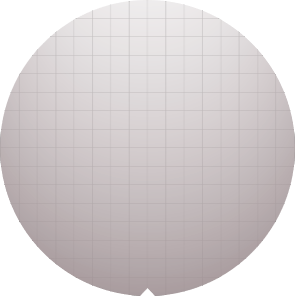
\includegraphics[scale=0.3]{structured_wafer.png}};
        \node[visible on=<2->, above=\y of sort] (sort_img) {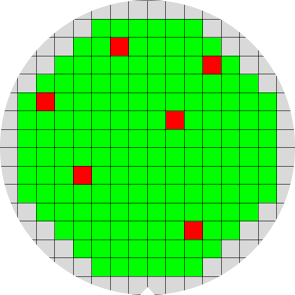
\includegraphics[scale=0.3]{sort.png}};
        \node[visible on=<3->, above=\y of die_bank] (die_bank_img) {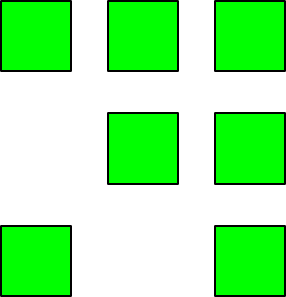
\includegraphics[scale=0.23]{die_bank.png}};
        \node[visible on=<4->, above=\y of assemble] (assembly_img) {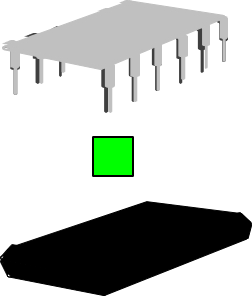
\includegraphics[scale=0.3]{assembly.png}};
        \node[visible on=<5->, above=\y of test] (test_img) {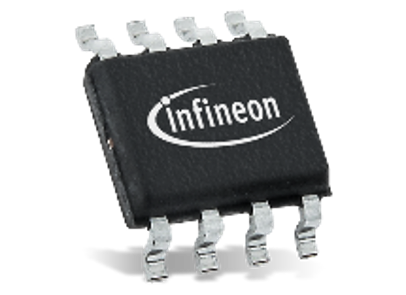
\includegraphics[scale=0.3]{test.png}};
        \node[visible on=<6->, above=\y of dc] (dc_img) {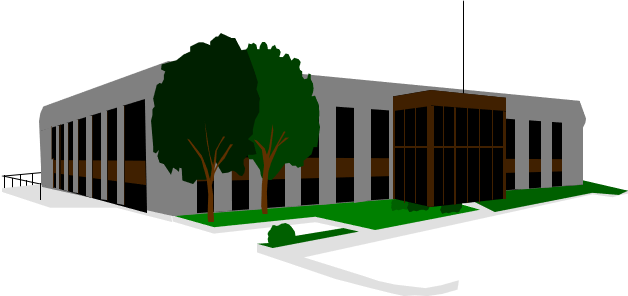
\includegraphics[scale=0.24]{distribution.png}};
        
        \end{tikzpicture}
    \end{center}
\end{frame}

\begin{frame}{Scanning Electron Microscope}
\begin{figure}
    \hspace{15mm}
        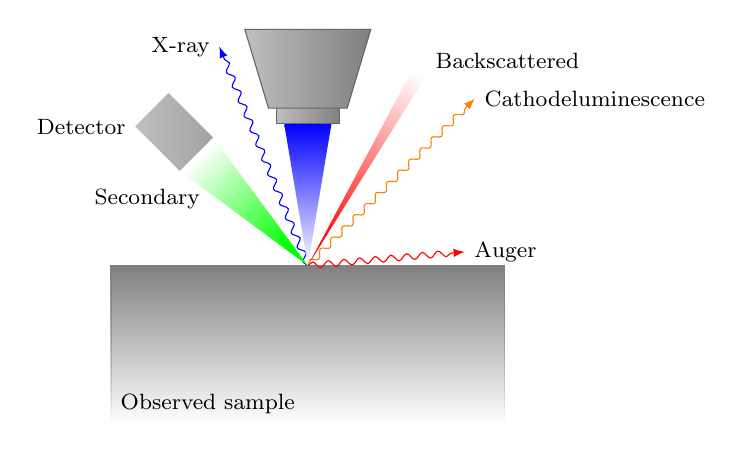
\begin{tikzpicture}
          \draw[gray,fill=gray,path fading=south] (0,0) rectangle +(5,-2);% sample
            \begin{scope}[decoration={snake,amplitude=.4mm,
                segment length=2mm,post length=1mm}]
              \draw[decorate,blue,->] (2.5,0) -- ++(112:3);% x-ray
              \draw[decorate,red,->] (2.5,0) -- ++(5:2);% auger
              \draw[decorate,orange,->] (2.5,0) -- ++(45:3);% cathodlimuescence
            \end{scope}
          \fill[color=red, path fading=north,fading transform={rotate=-15}]
            (2.5,0) ++(60:3) ++(150:0.1) -- ++(-30:0.2) -- (2.5,0) -- cycle;%backscatter
          \fill[color=green, path fading=north,fading transform={rotate=45}]
            (2.5,0) ++(135:2) ++(225:0.3) -- ++(45:0.6) -- (2.5,0) -- cycle;%secondary
          \shade[inner color=blue, top color=blue] (2.2,1.8)
            -- ++(0.6,0) -- ++(-0.3,-1.8) -- cycle;%primary occhelectrons
        
          \shade[left color=gray!50!white,right color=gray] (1.7,3)
            -- ++(1.6,0) -- ++(-0.3,-1) -- ++(-1,0) -- cycle;% column
          \shade[left color=gray!50!white,right color=gray] (2.1,2)
            -- ++(0.8,0) -- ++(0,-0.2) -- ++(-0.8,0) -- cycle;% column bottom
          \draw[gray!80!black] (1.7,3) -- ++(1.6,0) -- ++(-0.3,-1)
            -- ++(-1,0) -- cycle;%column
          \draw[gray!80!black] (2.1,2) -- ++(0,-0.2) -- ++(0.8,0)
            -- ++(0,0.2);%column bottom
        		
          \shade[left color=gray!50!white,right color=gray] (2.5,0) ++(135:2) --
            ++(225:0.3) -- ++(135:0.8) -- ++(45:0.6) -- ++(315:0.8) -- cycle;% detector
        		
          %labels
          \draw (0,-2) node[above right] {\footnotesize Observed sample};
          \draw (2.5,0) ++(5:2) node[right] {\footnotesize Auger};
          \draw (2.5,0) ++(45:3) node[right] {\footnotesize Cathodeluminescence};
          \draw (2.5,0) ++(60:3) node[right] {\footnotesize Backscattered};
          \draw (2.5,0) ++(112:3) node[left] {\footnotesize X-ray};
          \draw (2.5,0) ++(135:1.2) node[left=0.4cm] {\footnotesize Secondary};
          \draw (2.5,0) ++(135:2) ++(225:0.3) ++(135:0.8) node[left]
            {\footnotesize Detector};
        \end{tikzpicture}
        \caption*{Scanning electron microscope (SEM)}
\end{figure}   
\begin{flushright}
  \tiny{\textcolor{gray}{https://texample.net/tikz/examples/scanning-electron-microscopy/}}
\end{flushright}
\end{frame}

\begin{frame}{SEM Inspection}
    \begin{center}
        \begin{tikzpicture}
            % Fab process flow at the bottom of the figure
            \node[visible on=<1->, inner sep=0mm] (raw_wafer_img) at (1.1,1.75) {
\includegraphics[scale=0.17]{raw_wafer.png}};
            \node[visible on=<1->, step_rectangle, right=\step of raw_wafer_img] (step1)  {Step 1};
            \node[visible on=<1->, step_rectangle, right=\step of step1] (step2)  {Step 2};
            \node[visible on=<1->, step_rectangle, right=\step of step2] (step3)  {\ldots};
            \node[visible on=<1->, step_rectangle, right=\step of step3] (stepn)  {Step n};
            \node[visible on=<1->, inner sep=0mm, right=\step of stepn] (wafer_img) {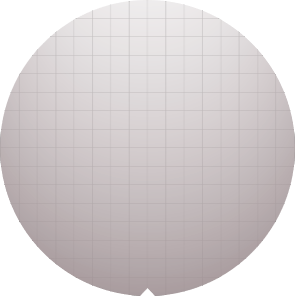
\includegraphics[scale=0.17]{structured_wafer.png}};
            
            % Arrows lining the fab process flow at the bottom of the figure
            \draw[visible on=<1->, arrow_small] (raw_wafer_img) -- (step1);
            \draw[visible on=<1->, arrow_small] (step1) -- (step2);
            \draw[visible on=<1->, arrow_small] (step2) -- (step3);
            \draw[visible on=<1->, arrow_small] (step3) -- (stepn);
            \draw[visible on=<1->, arrow_small] (stepn) -- (wafer_img);
                
            % Arrow from Step 1 to the SEM tool
            \draw[visible on=<2->, arrow_small] (3.2,2.15) |- (2.1,2.65) -| (2.1,3.15);
            % SEM tool
            \node[visible on=<2->, inner sep=0mm] (sem_tool) at (2.1,3.95) {
\includegraphics[scale=0.25]{sem_tool.png}};
            % SEM tool text
            \node[visible on=<2->, align=center, text=textfigurecolor] at (2.25,3.85) {\scriptsize SEM};            

            % SEM images box
            \node [visible on=<4->, rectangle, font=\scriptsize, rounded corners, minimum width=7.02cm, minimum height=3.02cm, draw=outlinecolor, fill=outlinecolor, right=\img of sem_tool, xshift = 0.2cm, yshift = 0.32cm] (image_box) {};
            
            % Arrow from the SEM tool to the image box
            \draw[visible on=<3->, arrow_small] (2.9,3.95) -- (3.27,3.95);
            
            % SEM image Class A
            \node[visible on=<3->, line width=0.2mm, draw=white, inner sep=0mm, right=\img of sem_tool, xshift = 0.37cm] (img1) {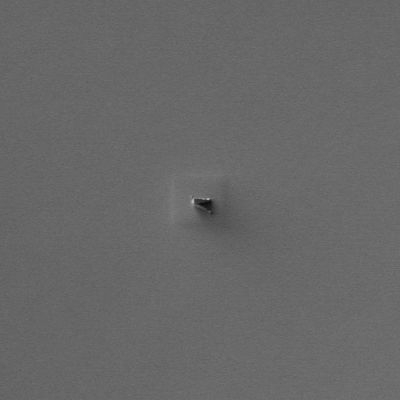
\includegraphics[height=2cm]{defect_1.jpg}};
            % SEM image Class B
            \node[visible on=<3->, line width=0.2mm, draw=white, inner sep=0mm, right=\img of img1] (img2) {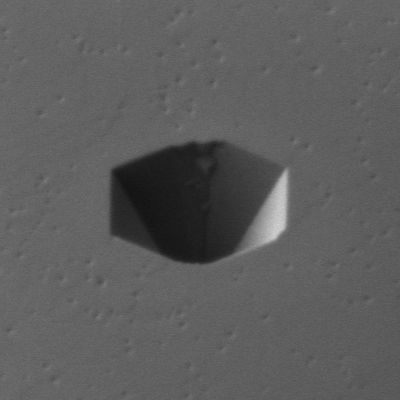
\includegraphics[height=2cm]{defect_2.jpg}};
            % SEM image Class C
            \node[visible on=<3->, line width=0.2mm, draw=white, inner sep=0mm, right=\img of img2] (img3)
            {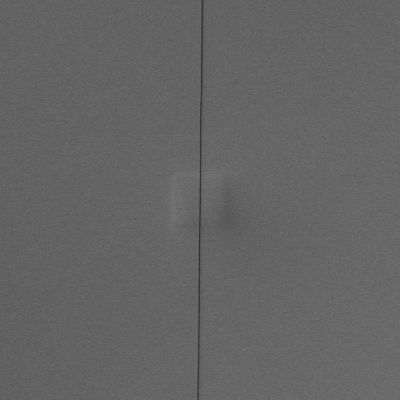
\includegraphics[height=2cm]{defect_3.jpg}};

            % SEM image labels for internal use
            \node[visible on=<4->, above=\adc of img1, text=textfigurecolor, font=\fontsize{10}{24}\selectfont] (class_1)  {Particle};
            \node[visible on=<4->, above=\adc of img2, text=textfigurecolor, font=\fontsize{10}{24}\selectfont] (class_2)  {Pit};
            \node[visible on=<4->, above=\adc of img3, text=textfigurecolor, font=\fontsize{10}{24}\selectfont] (class_3)  {Crack}; 

            % Novelties images box
            \node [visible on=<5->, rectangle, font=\scriptsize, rounded corners, minimum width=2.7cm, minimum height=3.02cm, draw=outlinecolor, fill=outlinecolor, right=\img of sem_tool, xshift = 7.9cm, yshift = 0.32cm] (image_box) {};
            
            % SEM images Novelties
            \node[visible on=<5->, line width=0.2mm, draw=white, inner sep=0mm,right=\imgfinal of img3, xshift = 0.2cm, yshift = 0.2cm] (img6) {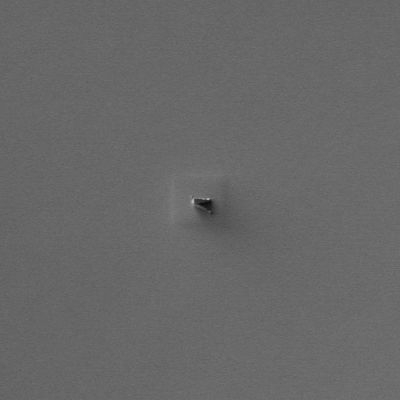
\includegraphics[height=2cm]{defect_4.jpg}};
            \node[visible on=<5->, line width=0.2mm, draw=white, inner sep=0mm,right=\imgfinal of img3, xshift = 0.1cm, yshift = 0.1cm] (img5) {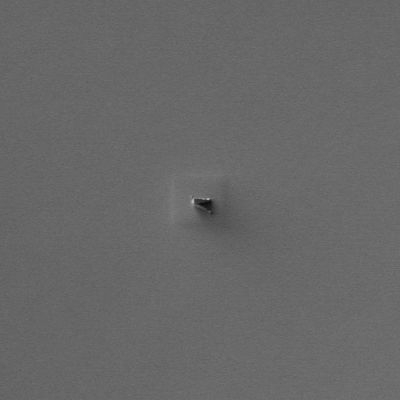
\includegraphics[height=2cm]{defect_4.jpg}};
            \node[visible on=<5->, line width=0.2mm, draw=white, inner sep=0mm,right=\imgfinal of img3] (img4) {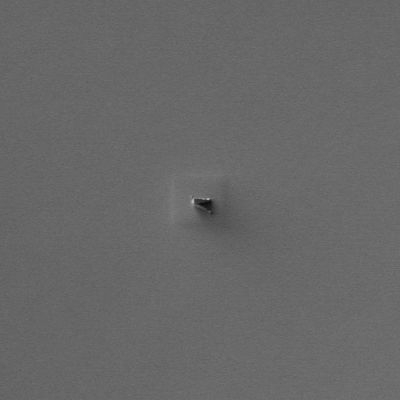
\includegraphics[height=2cm]{defect_4.jpg}};

            % Novelty overlay
            \node [visible on=<5->, novelty] at (img4) {?};

            % SEM image labels for internal and external use
            \node[visible on=<5->, above=\adc of img4, xshift = 0.1cm,  text=textfigurecolor, font=\fontsize{10}{24}\selectfont] (dc_adc_4)  {Novelties};
             
            % Arrow from the image box to the database
            \draw[visible on=<5->, arrow_small]  (10.55,3.95) -- (10.85,3.95);
            
            % Database
            %\node[visible on=<6->, inner sep=0pt,right=\img of img4, xshift = 0.57cm] (database) {
\includegraphics[scale=0.25]{database.png}};
        \end{tikzpicture}
    \end{center}
\end{frame}

\section{Theoretical Background}
%\begin{frame}{Classification Task}
    \begin{definitionblock}{Definition}
        \centering
        \begin{itemize}
            \item<1-> Dataset $\mathcal{D}$: set of input-output pairs
            \[
                \mathcal{D} = {\{(\mathbf{x}_i, y_i)\}}_{i=1}^n\,,
            \]
            where $\mathbf{x}_i \in \mathcal{X}$ is an input vector and $y_i\in \mathcal{Y} = \{c_1, \dots, c_K\}$ is its corresponding label;
            \item<2-> $y_i$ can be transformed in vector form $\mathbf{y}_i\in \mathcal{Y} = {\{0,1\}}^K$ using one-hot encoding:
            \[
                y_{ij} = 
                \begin{cases}
                    1, \text{if $\mathbf{x}_i$ has label $c_j$}\\
                    0, \text{otherwise}\,.
                \end{cases}
            \]
        \end{itemize}
    \end{definitionblock}
\end{frame}

\begin{frame}{Classification Task}
    \begin{definitionblock}{Definitions}
        \centering
        \begin{itemize}
            \item<1-> Underlying mapping $f$: a function
            \[
                f:\mathcal{X} \to \mathcal{Y}
            \]
            that maps input vectors to output labels.
        \end{itemize}
    \end{definitionblock}
\end{frame}

\begin{frame}{Classification Task}
    \begin{normalblock}{Classification Aim}
        \centering
        \begin{itemize}
            \item<1-> Given input $\mathbf{x}_i$, aim is to correctly predict label $\mathbf{y}_i$.
            \item<2-> Training process: $f$ is approximated using a parametrized function $f_{\theta}$:
            \[
                f_{\theta}: \mathcal{X} \to \mathcal{Y}\;,
            \]
            that minimizes the \emph{empirical risk}: 
            \[
                \mathcal{R}_{\epsilon}(\theta) \coloneqq \frac{1}{n}\sum_{i=1}^{n} L(\mathbf{y}_i,f_{\theta}(\mathbf{x_i}))\,.
            \]
        \end{itemize}
    \end{normalblock}
\end{frame}

\begin{frame}{Loss Function}
    \begin{definitionblock}{Definition}
        \centering
        \begin{itemize}
            \item<1-> Loss function $L$: measures the dissimilarity between predicted and true labels.
            \item<2-> Different possibilities:
            \begin{align*}
                L_{0, 1} &= \frac{1}{n} \sum_{i=1}^{n} \mathbb{I}(y_i, f_{\theta}(\mathbf{x}_i))\\
                L_{RMSE} &= \frac{1}{n}\sqrt{\sum_{i=1}^{n} {(y_i-f_{\theta}(\mathbf{x}_i))}^2}   
            \end{align*}
        \end{itemize}
    \end{definitionblock}
\end{frame}

\begin{frame}{Artificial Neural Network}
    \begin{figure}
        \centering
        \scalebox{0.7}{
        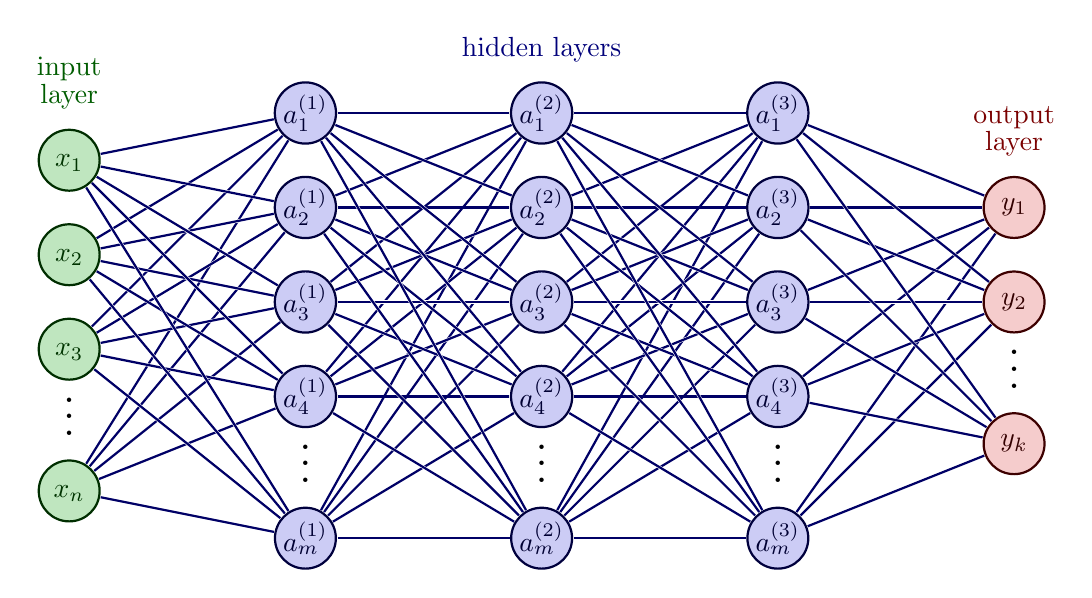
\begin{tikzpicture}[x=3cm,y=1.2cm]
            \message{^^JNeural network, shifted}
            \readlist\Nnod{4,5,5,5,3} % array of number of nodes per layer
            \readlist\Nstr{n,m,m,m,k} % array of string number of nodes per layer
            \readlist\Cstr{\strut x,a^{(\prev)},a^{(\prev)},a^{(\prev)},y} % array of coefficient symbol per layer
            \def\yshift{0.5} % shift last node for dots
            
            \message{^^J  Layer}
            \foreachitem \N \in \Nnod{ % loop over layers
            \def\lay{\Ncnt} % alias of index of current layer
            \pgfmathsetmacro\prev{int(\Ncnt-1)} % number of previous layer
            \message{\lay,}
            \foreach \i [evaluate={\c=int(\i==\N); \y=\N/2-\i-\c*\yshift;
                        \index=(\i<\N?int(\i):"\Nstr[\lay]");
                        \x=\lay; \n=\nstyle;}] in {1,...,\N}{ % loop over nodes
                % NODES
                \node[node \n] (N\lay-\i) at (\x,\y) {$\Cstr[\lay]_{\index}$};
                
                % CONNECTIONS
                \ifnum\lay>1 % connect to previous layer
                \foreach \j in {1,...,\Nnod[\prev]}{ % loop over nodes in previous layer
                    \draw[connect,white,line width=1.2] (N\prev-\j) -- (N\lay-\i);
                    \draw[connect] (N\prev-\j) -- (N\lay-\i);
                    %\draw[connect] (N\prev-\j.0) -- (N\lay-\i.180); % connect to left
                }
                \fi % else: nothing to connect first layer
                
            }
            \path (N\lay-\N) --++ (0,1+\yshift) node[midway,scale=1.5] {$\vdots$};
            }
            
            % LABELS
            \node[above=0.1,align=center,mygreen!60!black] at (N1-1.90) {input\\[-0.2em]layer};
            \node[above=0.1,align=center,myblue!60!black] at (N3-1.90) {hidden layers};
            \node[above=0.1,align=center,myred!60!black] at (N\Nnodlen-1.90) {output\\[-0.2em]layer};
            
        \end{tikzpicture}
        }
        \caption*{Test}
    \end{figure}
\end{frame}

\section{Methodology}
%\begin{frame}{Dataset Overview}
 \begin{center}
    \begin{figure}
    \centering
     \begin{tikzpicture}
        % Sample image and dimensions
         \node[visible on=<1->, step_rectangle] at (0,5.9) (sample) {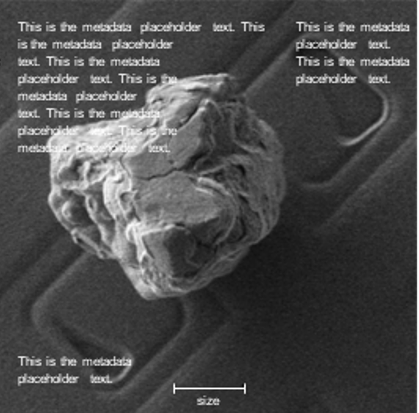
\includegraphics[scale=0.4]{sample_defect.png}};
        \draw[decoration={mirror,raise=3mm},decorate] (-2.6,8.2) -- (-2.6,3.6) node[left,midway] {480};
        \draw[decoration={mirror,raise=-3mm},decorate] (-2.3,3.33) -- (2.3,3.33) node[below,midway] {480};

        % Metadata boxes
        \node[visible on=<2->, right=\imgfinal of sample, step_rectangle, xshift = 1.5cm, yshift = 1.5cm] (firstrectcenter) {Technology};
        \node[visible on=<2->, left=\img of firstrectcenter, step_rectangle] (firstrectleft) {...};
        \node[visible on=<2->, right=\img of firstrectcenter, step_rectangle] (firstrectright) {...};
        
        \node[visible on=<3->, right=\imgfinal of sample, step_rectangle, xshift = 1.65cm, yshift = 0cm] (secondrectcenter) {Product};
        \node[visible on=<3->, left=\img of secondrectcenter, step_rectangle] (secondrectleft) {...};
        \node[visible on=<3->, right=\img of secondrectcenter, step_rectangle] (secondrectright) {...};
        
        \node[visible on=<4->, right=\imgfinal of sample, step_rectangle, xshift = 1.5cm, yshift = -1.5cm] (thirdrectcenter) {Step/Layer};
        \node[visible on=<4->, left=\img of thirdrectcenter, step_rectangle] (thirdrectleft) {...};
        \node[visible on=<4->, right=\img of thirdrectcenter, step_rectangle] (thirdrectright) {...};

        %  Arrows
        \draw[visible on=<3->, arrow_small] (firstrectcenter) -- (secondrectcenter);
        \draw[visible on=<3->, arrow_small] (firstrectcenter) -- (secondrectleft);
        \draw[visible on=<3->, arrow_small] (firstrectcenter) -- (secondrectright);
        
        \draw[visible on=<4->, arrow_small] (secondrectcenter) -- (thirdrectcenter);
        \draw[visible on=<4->, arrow_small] (secondrectcenter) -- (thirdrectleft);
        \draw[visible on=<4->, arrow_small] (secondrectcenter) -- (thirdrectright);
        
     \end{tikzpicture}
     \caption*{\hspace*{4em} Image dimensions \uncover<2->{\hspace*{7em} Correlated metadata}}

     \end{figure}
 \end{center}
\end{frame}

\begin{frame}{Dataset Distribution}
  \begin{figure}[h]
    \centering
        \resizebox{9cm}{!}{
        \begin{tikzpicture}[font=\small]
            \pgfplotsset{every axis/.append style={
                axis x line=middle,    % put the x axis in the middle
                axis y line=middle,    % put the y axis in the middle
                axis line style={-}, % arrows on the axis
                label style={font=\small},
                tick label style={font=\tiny},
                },}
            \begin{axis} [ybar,
              bar width=3.1mm,
              ymin=0,
              ymax=1500,
              xtick=data,
              axis x line=bottom,
              axis y line=left,
              enlarge x limits=0.02,
              x=0.31cm,
              ylabel={Samples}, 
              xlabel={Label},
              x label style={at={(axis description cs:0.5,-0.1)},anchor=north},
              y label style={at={(axis description cs:-0.05,.5)},rotate=90,anchor=south},                    
              ]
              \only<2->{\draw[dashed, maincolor] (axis cs:0, 500) -- (axis cs:37.5, 500);}
              \only<1>{\addplot[scatter,scatter src=y,mark=ybar, fill = plotcolor, draw=maincolor] coordinates {
                (1,441)
                (2,136)
                (3,168)
                (4,415)
                (5,1492)
                (6,1410)
                (7,58)
                (8,309)
                (9,85)
                (10,95)
                (11,174)
                (12,375)
                (13,156)
                (14,408)
                (15,190)
                (16,286)
                (17,337)
                (18,477)
                (19,101)
                (20,372)
                (21,659)
                (22,630)
                (23,256)
                (24,50)
                (25,168)
                (26,52)
                (27,988)
                (28,209)
                (29,830)
                (30,212)
                (31,168)
                (32,92)
                (33,83)
                (34,51)
                (35,417)
                (36,131)
                (37,128)
              };}
              \only<2>{\addplot[scatter,scatter src=y,mark=ybar, fill = plotcolor, draw=maincolor] coordinates {
                (1,441)
                (2,136)
                (3,168)
                (4,415)
                (5,1492)
                (6,1410)
                (7,58)
                (8,309)
                (9,85)
                (10,95)
                (11,174)
                (12,375)
                (13,156)
                (14,408)
                (15,190)
                (16,286)
                (17,337)
                (18,477)
                (19,101)
                (20,372)
                (21,659)
                (22,630)
                (23,256)
                (24,50)
                (25,168)
                (26,52)
                (27,988)
                (28,209)
                (29,830)
                (30,212)
                (31,168)
                (32,92)
                (33,83)
                (34,51)
                (35,417)
                (36,131)
                (37,128)
              };}
              \only<3>{\addplot[scatter,scatter src=y,mark=ybar, fill = plotcolor, draw=maincolor] coordinates {
                (1,441)
                (2,136)
                (3,168)
                (4,415)
                (5,500)
                (6,500)
                (7,58)
                (8,309)
                (9,85)
                (10,95)
                (11,174)
                (12,375)
                (13,156)
                (14,408)
                (15,190)
                (16,286)
                (17,337)
                (18,477)
                (19,101)
                (20,372)
                (21,500)
                (22,500)
                (23,256)
                (24,50)
                (25,168)
                (26,52)
                (27,500)
                (28,209)
                (29,500)
                (30,212)
                (31,168)
                (32,92)
                (33,83)
                (34,51)
                (35,417)
                (36,131)
                (37,128)
              };}
              \only<4>{\addplot[scatter,scatter src=y,mark=ybar, fill = plotcolor, draw=maincolor] coordinates {
                (1,500)
                (2,500)
                (3,500)
                (4,500)
                (5,500)
                (6,500)
                (7,500)
                (8,500)
                (9,500)
                (10,500)
                (11,500)
                (12,500)
                (13,500)
                (14,500)
                (15,500)
                (16,500)
                (17,500)
                (18,500)
                (19,500)
                (20,500)
                (21,500)
                (22,500)
                (23,500)
                (24,500)
                (25,500)
                (26,500)
                (27,500)
                (28,500)
                (29,500)
                (30,500)
                (31,500)
                (32,500)
                (33,500)
                (34,500)
                (35,500)
                (36,500)
                (37,500)
              };}
              
              \end{axis}
        \end{tikzpicture}
        }\hspace*{1em}
    \only<1>{\caption*{Initial defect class distribution}}
    \only<2>{\caption*{Initial defect class distribution}}
    \only<3>{\caption*{Downsampled defect class distribution}}
    \only<4>{\caption*{Resampled (upsampled \& downsampled) defect class distribution}}
    \end{figure}
\end{frame}
    
\begin{frame}{Data Augmentation}
    \begin{table}[h]
        \noindent
        \makebox[\linewidth]{
          \centering
          \begin{tabular}{SSS}
          \toprule
          {\textbf{Name}} & {\textbf{Description}} & {\textbf{Value}}   \\ \midrule
          {Horizontal flip}  & {Mirror the image on the x-axis}              & {\{True, False\}} \\ 
          {Vertical flip}    & {Mirror the image on the y-axis}              & {\{True, False\}} \\
          {Rotation}         & {Rotate the image with respect to its center} & {$[-90, 90]$}\\ 
          {Zoom}             & {Zoom in} & {$[1, 1.3]$} \\ 
          {Horizontal shift} & {Shift the image horizontally}                & {$[-0.5, 0.5]$} \\
          {Vertical shift}   & {Shift the image vertically}                  & {$[-0.5, 0.5]$} \\
          \bottomrule
          \end{tabular}
          }
          \caption*{Transformations applied to images}
    \end{table}
\end{frame}

\begin{frame}{Backbone Architecture: ResNet50}
    \begin{figure}
        \centering
        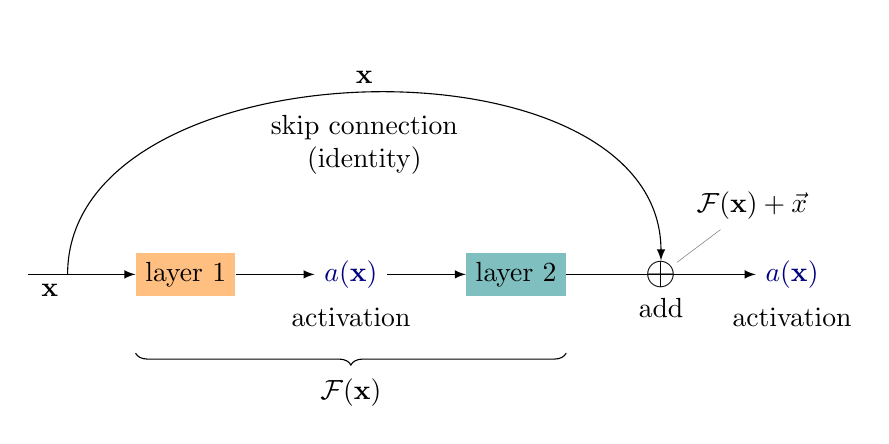
\begin{tikzpicture}
            \node[fill=orange!50] (l1) {layer 1};
            \node[blue!50!black, right=of l1, label={below:activation}] (act1) {$a(\mathbf{x})$};
            \node[fill=teal!50, right=of act1] (l2) {layer 2};
            \node[right=of l2, font=\Large, label={below:add}, inner sep=0, pin={60:$\mathcal F(\mathbf{x}) + \vec x$}] (add) {$\oplus$};
            \node[blue!50!black, right=of add, label={below:activation}] (act2) {$a(\mathbf{x})$};
          
            \draw[->] (l1) -- (act1);
            \draw[->] (act1) -- (l2);
            \draw[<-] (l1) -- ++(-2,0) node[below, pos=0.8] {$\mathbf{x}$};
            \draw[->] (l2) -- (act2) node[above, pos=0.8] {};
            \draw[->] ($(l1)-(1.5,0)$) to[out=90, in=90] node[below=1ex, midway, align=center] {skip connection\\(identity)} node[above, midway] {$\mathbf{x}$} (add);
            \draw[decorate, decoration={brace, amplitude=1ex, raise=1cm}] (l2.east) -- node[midway, below=1.2cm] {$\mathcal F(\mathbf{x})$} (l1.west);
          
        \end{tikzpicture}
        \caption*{Residual block}
    \end{figure}
\end{frame}

\begin{frame}{Backbone Architecture: EfficientNet}
    \begin{figure}
        \centering
            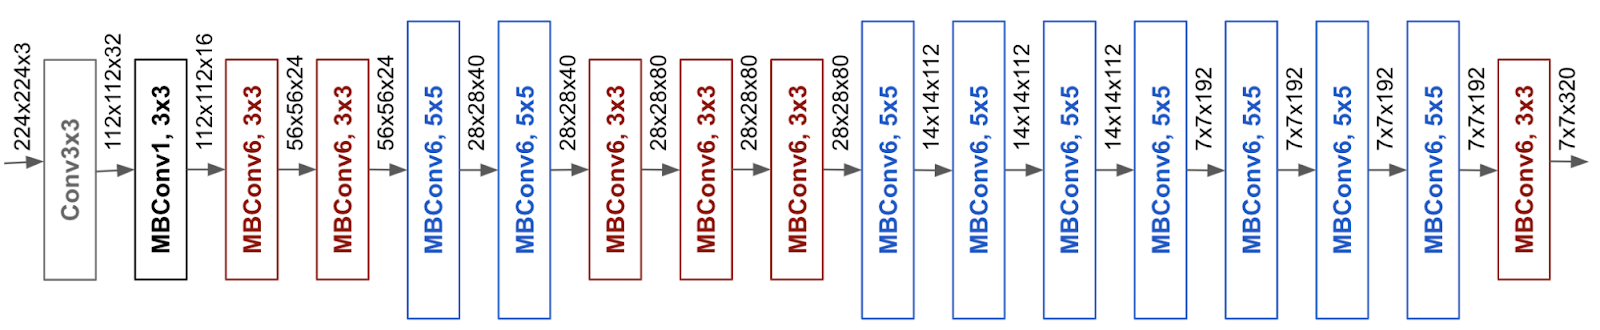
\includegraphics[scale=0.35]{effnet_pic.png}
            \caption*{EfficientNets}
    \end{figure}
\end{frame}

\begin{frame}{Dataset Subdivision}
    \begin{normalblock}{Unknown generation}
        \begin{itemize}
          \item No unknown class can be present in the dataset.
          \item For methodology testing purposes, dataset is divided in $\mathcal{K}$ and $\mathcal{U}$.
        \end{itemize}
    \end{normalblock}

    \begin{table}
        \noindent
        \makebox[\linewidth]{
            \centering
            \begin{tabular}{SSS}
            \toprule
            {\textbf{Name}} & {\textbf{Symbol}} & {\textbf{Composition}} \\ \midrule
            {Training set} & {$\mathcal{D}_{train}$} & {70\% of $\mathcal{K}$'s samples}\\
            {Validation set} & {$\mathcal{D}_{val}$} & {20\% of $\mathcal{K}$'s samples}\\
            {In-test set} & {$\mathcal{D}^{\mathcal{K}}_{test}$} & {10\% of $\mathcal{K}$'s samples}\\
            {Out-test set} & {$\mathcal{D}^{\mathcal{U}}_{test}$} & {100\% of $\mathcal{U}$'s samples}\\
            \bottomrule
            \end{tabular}
        }
        \caption*{Subsets of the original dataset}
    \end{table}
\end{frame}

\begin{frame}{Distance Method with Ground Truth}
    \begin{minipage}[c]{0.5\textwidth}
        \centering
        \vspace*{15px}
        \begin{overprint}
            \onslide<1-5>\begin{normalblock}{Method steps}
                \begin{itemize}
                    \item <1-> Backbone trained on $\mathcal{D}_{train}$.
                    \item <2-> Latent representations $\mathcal{S}_{train} = {\{\mathbf{s}_i\}}_{i=1}^{n_1}$ of $\mathcal{D}_{train}$ extracted.
                    \item <3-> Clusters $\mathcal{C} = {\{c_j\}}_{j=1}^{|\mathcal{K}|}$ formed using ground truth labels.
                    \item <4-> Centroids $\mathbf{\mu}_j$ found for each cluster.
                    \item <5-> Distances $d_{i,j}$ from centroids evaluated.
                \end{itemize}
            \end{normalblock}
            \onslide<6->\begin{normalblock}{Method steps}
              \begin{itemize}
                  \item <6-> Distance $\bar{d_j}$ found $\forall j$, corresponding to chosen $P$-th percentile.
                  \item <7-> $\mathbf{x} \in \mathcal{D}_{test}$ fed to the backbone. 
                  \item <8-> Distances $\hat{d_j}$ from centroids evaluated.
                  \item <9-> $\mathbf{x}$ classified as unknown if: 
                  \[
                      \hat{d_j} > \bar{d_j} \quad \forall j=1, \dots, |\mathcal{K}|\,.
                  \]
              \end{itemize}
          \end{normalblock}
        \end{overprint}
    \end{minipage}
    \begin{minipage}[c]{0.4\textwidth}
        \hspace*{50px}
        \centering
        \scalebox{.73}{
        \onslide<2->\begin{tikzpicture}
                  
            \pgfplotsset{
                scale only axis,
            }
            
            \begin{axis}[
              xmin=0.4, 
              xmax=1, 
              ymin=0.5, 
              ymax=1.1,
              x=10cm,
              y=10cm,
              ticks=none]
              \addplot[visible on=<2>, only marks, mark=asterisk, color=black]
              coordinates{
                (0.47,0.58)
                (0.52,0.57)
                (0.5,0.65)
                (0.45,0.62)
                (0.49,0.6)
              };
              \addplot[visible on=<2>, only marks, mark=asterisk, color=black]
              coordinates{
                (0.65,0.87)
                (0.66,0.89)
                (0.75,0.95)
                (0.72,0.98)
                (0.64,0.82)
              }; 
              \addplot[visible on=<2>, only marks, mark=asterisk, color=black]
              coordinates{
                (0.81,0.59)
                (0.88,0.57)
                (0.79,0.61)
                (0.85,0.63)
                (0.92,0.59)
              }; 

              \addplot[visible on=<3->, only marks, mark=asterisk, color=customgreen]
              coordinates{
                (0.47,0.58)
                (0.52,0.57)
                (0.5,0.65)
                (0.45,0.62)
                (0.49,0.6)
              };
              \addplot[visible on=<3->, only marks, mark=asterisk, color=customblue]
              coordinates{
                (0.65,0.87)
                (0.66,0.89)
                (0.75,0.95)
                (0.72,0.98)
                (0.64,0.82)
              }; 
              \addplot[visible on=<3->, only marks, mark=asterisk, color=customred]
              coordinates{
                (0.81,0.59)
                (0.88,0.57)
                (0.79,0.61)
                (0.85,0.63)
                (0.92,0.59)
              }; 

              % centroids
              \addplot[visible on=<4->, only marks, mark=*, color=customgreen]
              coordinates{
                (0.486,0.604)
              }; 

              \addplot[visible on=<4->, only marks, mark=*, color=customblue]
              coordinates{
                (0.686,0.901)
              }; 

              \addplot[visible on=<4->, only marks, mark=*, color=customred]
              coordinates{
                (0.85,0.6)
              }; 
              
              % text
              \node[] at (axis cs: 0.45,1.05) {$\mathcal{X}$};
              \node[visible on=<2>] at (axis cs: 0.6,1) {$S_{train}$};
              \node[visible on=<3->, color=customblue] at (axis cs: 0.6,1) {$c_1$};
              \node[visible on=<3->, color=customgreen] at (axis cs: 0.5,0.7) {$c_2$};
              \node[visible on=<3->, color=customred] at (axis cs: 0.9,0.72) {$c_3$};
          
              % lines to centroids
              \addplot[visible on=<5->, color=customgreen] coordinates{(0.47,0.58) (0.486,0.604)};
              \addplot[visible on=<5->, color=customgreen] coordinates{(0.5,0.65) (0.486,0.604)};
              \addplot[visible on=<5->, color=customgreen] coordinates{(0.45,0.62) (0.486,0.604)};
              \addplot[visible on=<5->, color=customgreen] coordinates{(0.49,0.6) (0.486,0.604)};
              \addplot[visible on=<5>, color=customgreen] coordinates{(0.52,0.57) (0.486,0.604)};
              \addplot[visible on=<6->, color=black] coordinates{(0.52,0.57) (0.486,0.604)};

              \addplot[visible on=<5->, color=customblue] coordinates{(0.65,0.87) (0.686,0.901)};
              \addplot[visible on=<5->, color=customblue] coordinates{(0.66,0.89) (0.686,0.901)};
              \addplot[visible on=<5->, color=customblue] coordinates{(0.75,0.95) (0.686,0.901)};
              \addplot[visible on=<5->, color=customblue] coordinates{(0.72,0.98) (0.686,0.901)};
              \addplot[visible on=<5>, color=customblue] coordinates{(0.64,0.82) (0.686,0.901)};
              \addplot[visible on=<6->, color=black] coordinates{(0.64,0.82) (0.686,0.901)};

              \addplot[visible on=<5->, color=customred] coordinates{(0.81,0.59) (0.85,0.6)};
              \addplot[visible on=<5->, color=customred] coordinates{(0.88,0.57) (0.85,0.6)};
              \addplot[visible on=<5->, color=customred] coordinates{(0.79,0.61) (0.85,0.6)};
              \addplot[visible on=<5->, color=customred] coordinates{(0.85,0.63) (0.85,0.6)};
              \addplot[visible on=<5>, color=customred] coordinates{(0.92,0.59) (0.85,0.6)};
              \addplot[visible on=<6->, color=black] coordinates{(0.92,0.59) (0.85,0.6)};

              % outlier
              \addplot[visible on=<7-9>, only marks, mark=asterisk, color=black]
              coordinates{(0.7,0.7)}; 
              \addplot[visible on=<8-9>, color=black] coordinates{(0.7,0.7) (0.486,0.604)};
              \addplot[visible on=<8-9>, color=black] coordinates{(0.7,0.7) (0.686,0.901)};
              \addplot[visible on=<8-9>, color=black] coordinates{(0.7,0.7) (0.85,0.6)};
              \node[visible on=<9>] at (axis cs: 0.79,0.73) {\emph{unknown}};

              % outlier2
              \addplot[visible on=<10-12>, only marks, mark=asterisk, color=black]
              coordinates{(0.7,0.85)}; 
              \addplot[visible on=<11-12>, color=black] coordinates{(0.7,0.85) (0.486,0.604)};
              \addplot[visible on=<11-12>, color=black] coordinates{(0.7,0.85) (0.686,0.901)};
              \addplot[visible on=<11-12>, color=black] coordinates{(0.7,0.85) (0.85,0.6)};
              \node[visible on=<12>] at (axis cs: 0.78,0.87) {\emph{known}};

            \end{axis}
        \end{tikzpicture}
        }
    \end{minipage}
\end{frame}

\begin{frame}{Distance Method without Ground Truth}
    \centering
    \begin{normalblock}{Method steps}
        \begin{itemize}
            \item \textcolor{black!20}{Backbone trained on $\mathcal{D}_{train}$.}
            \item \textcolor{black!20}{Latent representations $\mathcal{S}_{train} = {\{\mathbf{s}_i\}}_{i=1}^{n_1}$ of $\mathcal{D}_{train}$ extracted.}
            \item Clusters $\mathcal{C} = {\{c_j\}}_{j=1}^{|\mathcal{K}|}$ formed using \emph{clustering algorithms}.
            \item \textcolor{black!20}{Centroids $\mathbf{\mu}_j$ found for each cluster.}
            \item \textcolor{black!20}{Distances $d_{i,j}$ from centroids evaluated.}
        \end{itemize}
  \end{normalblock}
\end{frame}

\begin{frame}{Mahalanobis Distance}
  \begin{minipage}{0.47\textwidth}
      \centering
      \begin{definitionblock}{Definition}
          \begin{itemize}
              \item Let $\mathbf{\mu} = {(\mu_1, \dots, \mu_N)}^T$ be the centroid of a distribution $Q$ and $\Sigma$ its positive-definite covariance matrix. The Mahalanobis distance of a point $\mathbf{x}$ from Q is defined as:
              \[
                  d_M(\mathbf{x}, Q) = \sqrt{{(\mathbf{x}-\mathbf{\mu})}^T\Sigma^{-1}(\mathbf{x}-\mathbf{\mu})}\,.
              \]
          \end{itemize}
      \end{definitionblock}
  \vspace*{12px}
  \end{minipage}
  \quad
  \begin{minipage}{0.49\textwidth}
          \begin{figure}[h]
              \centering
              \scalebox{.63}{
                  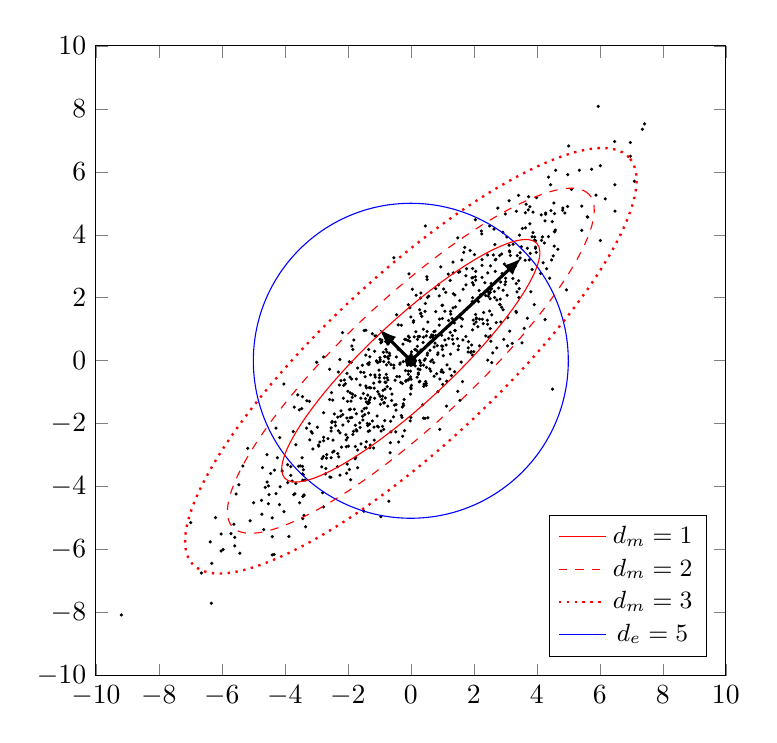
\begin{tikzpicture}
                  
                      \pgfplotsset{
                          scale only axis,
                      }
                      
                      \begin{axis}[
                        xmin=-10, 
                        xmax=10, 
                        ymin=-10, 
                        ymax=10,
                        %axis equal image
                        x=0.4cm,
                        y=0.4cm,
                        %ticks=none,
                        legend style={font=\small},
                        legend pos = south east
                        ]
                
                        \addlegendimage{color=red}
                        \addlegendentry{$d_m = 1$}
                
                        \addlegendimage{color=red, dash pattern=on 3pt off 3pt}
                        \addlegendentry{$d_m = 2$}
                
                        \addlegendimage{color=red, dash pattern=on \pgflinewidth off 2pt, line width=0.3mm}
                        \addlegendentry{$d_m = 3$}
                
                        \addlegendimage{color=blue}
                        \addlegendentry{$d_e = 5$}
                
                        %\addlegendentry{plot 2}
                
                        %\draw[rotate around={-35:(0.7,0.9)},blue, fill=blue, fill opacity=0.2] (0.7,0.9) ellipse (9pt and 15pt);
                        \begin{scope}[on background layer]
                        \addplot[ultra thin, only marks, mark=*, color=black, mark size = 0.35pt]
                        coordinates{
                          (3.35, 2.45)
                          (-2.27, -0.77)
                          (-1.73, -1.68)
                          (1.42, 1.71)
                          (2.99, 2.42)
                          (2.08, 1.36)
                          (-1.00, -0.54)
                          (1.01, 0.46)
                          (0.13, 0.36)
                          (4.89, 4.69)
                          (-1.08, -0.03)
                          (4.98, 5.91)
                          (-0.03, 1.68)
                          (-3.43, -4.31)
                          (-0.02, -1.91)
                          (2.54, 0.79)
                          (-1.71, -2.23)
                          (0.70, 0.81)
                          (0.52, 0.18)
                          (3.35, 1.53)
                          (1.12, 0.50)
                          (1.08, 0.66)
                          (3.99, 5.18)
                          (-0.76, 0.28)
                          (1.83, 0.61)
                          (-1.82, -2.24)
                          (-3.81, -3.64)
                          (-0.24, -0.03)
                          (0.35, 1.41)
                          (-0.74, 0.12)
                          (0.17, 2.08)
                          (-2.48, -2.90)
                          (1.39, -0.35)
                          (2.64, 4.18)
                          (4.24, 3.74)
                          (0.92, -2.18)
                          (0.55, 0.53)
                          (-3.36, -3.79)
                          (-2.68, -3.09)
                          (-1.93, -0.52)
                          (0.46, 4.28)
                          (-4.71, -3.39)
                          (-2.29, -3.05)
                          (0.77, 0.94)
                          (-4.03, -4.79)
                          (2.35, 2.48)
                          (-0.20, -2.22)
                          (2.88, 3.39)
                          (4.15, 3.82)
                          (0.95, 2.98)
                          (0.20, -0.52)
                          (-0.48, -2.26)
                          (-2.71, -3.59)
                          (-1.34, -1.35)
                          (3.44, 2.29)
                          (4.14, 4.63)
                          (0.73, 0.92)
                          (0.49, 0.79)
                          (3.12, 5.08)
                          (-0.97, 0.03)
                          (3.01, 2.51)
                          (-1.49, -0.37)
                          (-1.07, -1.75)
                          (0.50, -0.21)
                          (-1.84, 0.36)
                          (-1.58, -2.64)
                          (1.94, 2.63)
                          (5.60, 4.57)
                          (-2.23, -1.76)
                          (1.68, 3.44)
                          (4.98, 4.90)
                          (5.35, 6.05)
                          (2.70, 3.22)
                          (-4.40, -5.58)
                          (-1.18, -2.77)
                          (3.63, 3.19)
                          (1.96, 2.93)
                          (1.96, 2.48)
                          (-6.20, -4.98)
                          (2.79, 2.31)
                          (1.75, 2.70)
                          (2.05, 4.48)
                          (-1.69, -0.23)
                          (-1.77, -1.11)
                          (3.96, 3.57)
                          (-1.03, -2.10)
                          (1.32, 0.80)
                          (3.12, 3.67)
                          (-3.30, -1.27)
                          (2.26, 3.21)
                          (2.44, 0.02)
                          (1.00, 0.36)
                          (1.14, -0.65)
                          (1.66, 2.27)
                          (2.07, 1.23)
                          (-4.57, -2.98)
                          (-1.13, -0.52)
                          (-0.66, -2.92)
                          (1.19, 2.75)
                          (0.54, -1.81)
                          (-0.86, -1.34)
                          (2.95, 0.68)
                          (6.48, 5.59)
                          (1.20, 1.28)
                          (-6.02, -5.50)
                          (4.28, 4.69)
                          (1.96, 0.18)
                          (4.60, 6.05)
                          (-3.87, -5.58)
                          (-1.28, -0.45)
                          (-2.82, -3.11)
                          (-0.54, 3.27)
                          (3.42, 5.25)
                          (-1.31, -2.01)
                          (0.82, -0.41)
                          (0.21, 0.68)
                          (1.75, 0.77)
                          (0.01, -0.89)
                          (2.17, 2.23)
                          (0.99, 1.76)
                          (7.42, 7.52)
                          (-3.81, -3.36)
                          (-0.97, -1.38)
                          (-0.19, 0.68)
                          (2.82, 3.34)
                          (-1.09, -0.00)
                          (4.20, 3.11)
                          (0.62, 0.60)
                          (-2.25, -2.29)
                          (-2.77, -2.54)
                          (1.97, 2.64)
                          (-0.71, 0.07)
                          (1.77, 2.92)
                          (2.43, 1.29)
                          (2.67, 3.69)
                          (2.44, 2.79)
                          (2.97, 3.07)
                          (-0.80, 0.61)
                          (1.31, 1.34)
                          (-1.05, -0.98)
                          (-0.99, -0.45)
                          (-1.86, -1.16)
                          (0.57, 2.05)
                          (0.84, 0.48)
                          (3.37, 2.19)
                          (-1.92, -1.54)
                          (-1.69, -2.83)
                          (1.01, 1.76)
                          (3.78, 4.89)
                          (0.67, 0.77)
                          (3.88, 4.07)
                          (0.28, 0.77)
                          (-0.75, -0.54)
                          (-1.87, 0.47)
                          (0.91, 1.32)
                          (-5.59, -5.61)
                          (0.88, 2.41)
                          (3.76, 3.20)
                          (-1.90, -1.28)
                          (1.35, 2.79)
                          (-0.08, 1.78)
                          (-0.32, -0.69)
                          (-2.52, -1.01)
                          (-1.48, 0.96)
                          (-2.30, -0.36)
                          (-2.25, -3.63)
                          (-0.21, -1.23)
                          (-0.92, -1.23)
                          (-1.44, -1.20)
                          (-2.53, -2.23)
                          (-1.35, -2.24)
                          (-0.09, 0.65)
                          (2.44, 3.36)
                          (0.00, -1.80)
                          (-0.47, -1.57)
                          (2.88, 1.70)
                          (0.63, -0.33)
                          (0.96, -0.35)
                          (3.51, 3.62)
                          (2.26, 2.65)
                          (7.35, 7.35)
                          (2.54, 0.62)
                          (1.71, 3.60)
                          (3.73, 4.79)
                          (-1.29, -2.68)
                          (-2.51, -1.96)
                          (-1.33, -0.12)
                          (3.14, 0.94)
                          (0.40, -0.14)
                          (2.08, 1.33)
                          (-0.60, -1.06)
                          (-5.62, -5.19)
                          (2.13, 1.08)
                          (-3.22, -1.99)
                          (-2.48, -1.25)
                          (4.18, 3.93)
                          (3.00, 4.66)
                          (-0.55, -1.78)
                          (3.24, 2.61)
                          (-0.59, 0.67)
                          (-3.43, -3.79)
                          (-0.90, -2.08)
                          (4.47, 3.20)
                          (-6.32, -6.43)
                          (-2.47, -2.52)
                          (-4.28, -4.22)
                          (3.93, 3.93)
                          (-2.14, -1.19)
                          (-1.44, -2.74)
                          (4.94, 2.25)
                          (-3.59, -1.08)
                          (-2.16, -1.71)
                          (-1.35, -1.30)
                          (-0.01, -0.51)
                          (7.10, 5.70)
                          (1.04, 2.28)
                          (1.35, 0.54)
                          (-0.15, 0.67)
                          (0.79, 2.29)
                          (-2.58, -1.23)
                          (2.93, 2.24)
                          (-1.00, -0.67)
                          (0.17, 0.34)
                          (3.35, 4.75)
                          (-0.65, -0.89)
                          (2.06, 1.47)
                          (-0.34, -0.07)
                          (-2.16, -2.04)
                          (0.24, -0.39)
                          (-0.01, -1.06)
                          (-1.51, -1.04)
                          (0.77, 0.56)
                          (-5.96, -5.99)
                          (0.85, 0.20)
                          (-4.52, -4.54)
                          (3.98, 3.44)
                          (-2.53, -2.13)
                          (-1.48, -1.52)
                          (2.66, 2.01)
                          (0.74, -0.49)
                          (1.25, 0.90)
                          (-1.76, -2.72)
                          (-2.33, -3.36)
                          (-2.40, -1.95)
                          (-1.32, -0.85)
                          (1.56, -1.26)
                          (2.48, 2.12)
                          (-2.01, -1.29)
                          (-0.90, -1.12)
                          (2.83, 1.78)
                          (-1.54, -0.14)
                          (4.37, 3.94)
                          (0.68, 0.03)
                          (1.52, 2.81)
                          (2.38, 0.79)
                          (-1.32, -0.06)
                          (2.02, 3.37)
                          (2.53, 2.26)
                          (1.40, 2.09)
                          (-0.70, -0.05)
                          (-1.41, -2.57)
                          (-2.57, -3.69)
                          (0.23, -0.26)
                          (0.00, 1.39)
                          (0.92, -0.58)
                          (-1.93, -1.81)
                          (0.70, 0.64)
                          (-1.95, -0.03)
                          (-4.15, -4.00)
                          (-0.24, -1.37)
                          (3.96, 3.61)
                          (3.93, 3.83)
                          (2.68, 3.20)
                          (-3.41, -3.46)
                          (-1.37, -0.10)
                          (-1.75, -3.07)
                          (-1.22, -1.91)
                          (1.49, 3.90)
                          (-3.44, -1.14)
                          (6.02, 3.82)
                          (-0.79, 0.36)
                          (-5.33, -3.34)
                          (-3.40, -4.28)
                          (6.47, 6.96)
                          (-0.95, -4.95)
                          (3.47, 3.26)
                          (-2.53, -3.08)
                          (-3.44, -3.35)
                          (2.73, 1.93)
                          (4.54, 5.01)
                          (-0.92, 0.60)
                          (0.32, 1.51)
                          (0.53, 0.24)
                          (-3.51, -3.34)
                          (-2.32, -2.95)
                          (-1.31, -2.22)
                          (0.46, 0.06)
                          (-0.25, 0.53)
                          (-0.78, -0.43)
                          (-4.16, -2.44)
                          (1.99, 2.41)
                          (-0.87, 0.27)
                          (-0.03, 0.62)
                          (-0.83, -1.90)
                          (4.49, 4.42)
                          (-0.27, -0.72)
                          (-1.30, -2.76)
                          (1.27, 1.48)
                          (1.08, 1.57)
                          (-2.39, -2.06)
                          (-5.10, -5.08)
                          (-2.22, -1.59)
                          (-4.67, -5.36)
                          (-1.98, -1.92)
                          (-0.47, -1.39)
                          (-2.78, -3.04)
                          (1.90, 0.26)
                          (-1.06, -2.08)
                          (1.52, 0.47)
                          (1.62, 3.20)
                          (-3.91, -3.87)
                          (-0.39, -2.58)
                          (-0.79, -0.69)
                          (0.31, -0.15)
                          (-5.59, -5.88)
                          (0.14, -0.16)
                          (-2.01, -2.44)
                          (2.01, 1.17)
                          (-0.40, 0.36)
                          (-3.16, -2.25)
                          (2.47, 0.75)
                          (0.40, -1.82)
                          (-1.87, -1.80)
                          (1.00, 1.34)
                          (0.49, -0.78)
                          (3.22, 0.55)
                          (-6.02, -6.04)
                          (-2.70, -3.42)
                          (-0.46, 0.12)
                          (1.82, 0.41)
                          (0.11, -0.02)
                          (0.66, 0.82)
                          (-0.08, 0.78)
                          (1.25, 2.55)
                          (1.34, 1.68)
                          (1.61, 1.09)
                          (0.40, 1.00)
                          (-2.04, -3.57)
                          (0.73, -0.06)
                          (-1.76, -2.05)
                          (-2.05, -2.73)
                          (-5.18, -2.78)
                          (-0.81, -1.18)
                          (-0.05, 0.74)
                          (3.78, 4.35)
                          (3.05, 3.93)
                          (5.62, 4.56)
                          (5.43, 4.91)
                          (0.24, -0.43)
                          (0.32, 2.15)
                          (-1.05, -0.06)
                          (0.41, -0.81)
                          (0.32, 0.34)
                          (3.01, 2.62)
                          (-0.15, -0.63)
                          (0.31, -0.06)
                          (4.56, 4.67)
                          (3.64, 4.22)
                          (-4.56, -3.85)
                          (3.66, 4.97)
                          (-1.81, 0.66)
                          (2.25, 4.03)
                          (-6.37, -5.75)
                          (2.38, 2.07)
                          (0.79, 1.56)
                          (-3.73, -2.25)
                          (-3.46, -1.52)
                          (3.74, 5.21)
                          (3.43, 2.01)
                          (0.43, 0.02)
                          (5.01, 6.82)
                          (2.44, 1.16)
                          (2.31, 1.53)
                          (3.16, 3.34)
                          (2.26, 3.03)
                          (-1.17, -2.11)
                          (0.67, 0.78)
                          (0.98, -0.29)
                          (-4.52, -3.97)
                          (5.43, 4.14)
                          (0.46, 1.82)
                          (-0.36, -0.50)
                          (2.39, 2.21)
                          (0.21, 0.30)
                          (-3.39, -4.26)
                          (3.85, 3.94)
                          (2.15, 1.88)
                          (-0.54, -0.23)
                          (-4.28, -2.14)
                          (3.96, 3.81)
                          (-1.32, -1.33)
                          (-1.49, -4.78)
                          (-2.83, -3.37)
                          (4.37, 5.83)
                          (-0.06, -0.58)
                          (-2.93, -2.68)
                          (-1.16, -2.52)
                          (3.60, 1.03)
                          (0.05, 2.27)
                          (-1.15, -1.19)
                          (4.55, 3.64)
                          (-1.01, -0.30)
                          (0.47, -0.66)
                          (-0.61, -1.26)
                          (0.49, -0.72)
                          (0.90, 1.13)
                          (-3.65, -2.67)
                          (3.45, 3.99)
                          (-0.45, 1.46)
                          (-3.72, -4.25)
                          (-6.33, -7.70)
                          (-1.77, -3.11)
                          (-3.56, -3.35)
                          (-1.14, -0.45)
                          (-6.99, -5.14)
                          (4.44, 5.59)
                          (0.61, 0.33)
                          (1.11, 2.17)
                          (-0.92, 0.66)
                          (-3.22, -1.29)
                          (0.53, 2.01)
                          (0.02, 0.28)
                          (-2.77, -2.43)
                          (2.76, 4.85)
                          (4.56, 4.10)
                          (-3.65, -3.90)
                          (-2.77, -4.64)
                          (3.34, 1.57)
                          (0.70, 0.74)
                          (0.01, -0.59)
                          (-0.77, -0.13)
                          (4.59, 4.15)
                          (-4.99, -4.51)
                          (1.03, 0.16)
                          (-0.97, -1.13)
                          (-2.17, 0.89)
                          (-3.31, -2.14)
                          (0.63, -0.02)
                          (2.06, 2.56)
                          (2.55, 2.45)
                          (-0.86, -0.03)
                          (0.60, -0.26)
                          (1.64, -0.66)
                          (-0.50, -0.62)
                          (3.47, 3.43)
                          (1.35, 2.13)
                          (-3.43, -5.01)
                          (-0.71, 0.54)
                          (-1.34, -1.66)
                          (-1.43, 0.18)
                          (-1.84, -2.34)
                          (4.41, 2.62)
                          (1.38, 1.20)
                          (-1.28, -1.16)
                          (1.65, 0.66)
                          (-2.00, -0.97)
                          (1.50, 0.35)
                          (2.86, 1.23)
                          (2.68, 2.84)
                          (2.73, 0.41)
                          (4.52, 3.33)
                          (5.95, 8.08)
                          (0.38, -1.40)
                          (-2.13, -0.78)
                          (0.45, -1.83)
                          (1.49, -0.97)
                          (0.62, 0.75)
                          (0.40, 0.75)
                          (-1.95, -3.45)
                          (-1.18, -0.71)
                          (-1.37, -1.36)
                          (6.02, 6.19)
                          (-0.26, -2.40)
                          (4.67, 3.54)
                          (0.23, 0.77)
                          (1.34, 3.13)
                          (3.70, 1.35)
                          (3.07, 0.47)
                          (-4.40, -6.16)
                          (1.24, -0.26)
                          (1.20, 0.71)
                          (1.58, 1.37)
                          (3.88, 4.72)
                          (0.74, 0.44)
                          (-1.43, -0.80)
                          (0.27, -0.67)
                          (3.31, 3.00)
                          (3.38, 3.34)
                          (-0.82, -0.90)
                          (-2.02, -3.28)
                          (3.06, 2.08)
                          (1.64, 1.32)
                          (-4.40, -4.99)
                          (-0.82, -0.68)
                          (2.90, 2.77)
                          (-2.05, -2.51)
                          (-2.43, -1.69)
                          (-3.21, -2.51)
                          (-4.62, -4.02)
                          (4.12, 2.77)
                          (-1.95, -1.55)
                          (-2.50, -1.93)
                          (0.01, 0.21)
                          (-1.46, -1.71)
                          (1.60, -0.04)
                          (-1.69, -3.40)
                          (2.93, 1.62)
                          (-1.61, -0.77)
                          (2.21, 2.09)
                          (2.05, 2.67)
                          (-2.99, -0.05)
                          (2.62, 3.36)
                          (1.26, 0.21)
                          (-0.17, -0.31)
                          (-4.73, -4.87)
                          (-0.95, 0.57)
                          (-0.28, -1.80)
                          (-0.83, 0.14)
                          (-3.11, -2.80)
                          (-0.68, 0.24)
                          (-2.30, -2.22)
                          (-0.08, -0.43)
                          (0.86, -0.98)
                          (-1.92, -1.02)
                          (-3.91, -3.30)
                          (-0.54, -0.14)
                          (-0.73, -1.44)
                          (1.98, 1.29)
                          (-2.63, -2.47)
                          (-1.31, -1.24)
                          (-3.54, -1.56)
                          (-0.65, -2.60)
                          (0.54, 1.23)
                          (-2.22, -0.63)
                          (0.31, 1.49)
                          (-1.27, -0.86)
                          (-0.94, -2.23)
                          (0.51, 2.67)
                          (0.08, 1.22)
                          (2.92, 4.08)
                          (-1.01, -1.06)
                          (-0.23, -1.42)
                          (-1.74, -2.19)
                          (0.11, 0.76)
                          (-1.14, 0.79)
                          (-4.50, -4.25)
                          (2.71, 1.21)
                          (-0.83, 0.13)
                          (-0.40, 1.14)
                          (4.31, 2.92)
                          (1.29, -0.47)
                          (0.29, -0.65)
                          (-0.06, 2.76)
                          (-1.55, -1.60)
                          (-2.77, -1.65)
                          (-1.34, 0.36)
                          (-5.55, -4.23)
                          (-1.89, -0.05)
                          (3.25, 3.70)
                          (-1.16, -0.87)
                          (3.53, 0.57)
                          (2.24, 4.12)
                          (1.96, 2.00)
                          (-0.86, -2.18)
                          (4.57, 4.10)
                          (-0.16, -0.65)
                          (-1.73, -0.58)
                          (3.42, 2.54)
                          (1.55, 2.83)
                          (-5.46, -3.94)
                          (-3.45, -3.08)
                          (4.50, -0.90)
                          (2.06, 2.84)
                          (-1.91, -3.78)
                          (1.88, 3.50)
                          (3.92, 1.78)
                          (2.57, 1.46)
                          (-0.01, -0.33)
                          (0.39, 0.58)
                          (0.16, 0.92)
                          (1.32, 0.68)
                          (-0.11, -0.14)
                          (1.03, -0.37)
                          (0.90, 2.06)
                          (1.96, 0.98)
                          (-1.37, -1.09)
                          (-0.63, -2.26)
                          (-2.77, 0.12)
                          (-1.61, -2.12)
                          (0.29, -0.28)
                          (-3.68, -4.22)
                          (2.50, 1.58)
                          (-3.44, -3.59)
                          (2.00, 0.29)
                          (1.63, 1.50)
                          (-0.44, -0.50)
                          (-2.54, -3.70)
                          (3.54, 4.20)
                          (-1.15, 0.30)
                          (-2.58, -0.27)
                          (-2.97, -2.11)
                          (4.28, 4.65)
                          (2.85, 2.50)
                          (-6.65, -6.74)
                          (-1.09, 0.78)
                          (2.18, 1.32)
                          (-3.77, -3.82)
                          (-0.10, 0.12)
                          (-4.24, -3.08)
                          (4.45, 4.77)
                          (0.09, 1.27)
                          (-0.84, -1.33)
                          (-2.44, -2.87)
                          (0.98, 0.81)
                          (-2.03, -0.40)
                          (-1.98, -2.71)
                          (-1.30, 0.13)
                          (-3.39, -4.91)
                          (-0.88, -0.94)
                          (3.70, 3.57)
                          (0.00, -0.84)
                          (-3.34, -5.27)
                          (-4.74, -4.43)
                          (0.52, 2.58)
                          (1.13, -1.44)
                          (-4.09, -3.50)
                          (1.15, -0.13)
                          (2.84, 1.96)
                          (5.74, 6.08)
                          (-2.67, -2.98)
                          (-4.45, -3.58)
                          (-0.98, 0.10)
                          (6.97, 6.49)
                          (-0.64, -1.92)
                          (-3.53, -4.51)
                          (-1.45, -0.51)
                          (-1.85, -1.06)
                          (-0.75, -0.82)
                          (-0.08, -0.61)
                          (2.27, 1.32)
                          (2.18, 0.47)
                          (2.57, -0.06)
                          (-2.25, 0.04)
                          (-0.08, -0.33)
                          (0.45, 1.57)
                          (3.08, 1.37)
                          (-2.32, -1.79)
                          (0.86, 0.25)
                          (1.95, 1.88)
                          (-4.17, -4.57)
                          (6.17, 5.14)
                          (0.02, -0.78)
                          (0.21, 0.46)
                          (-1.59, -0.36)
                          (-2.20, -2.74)
                          (1.40, 0.96)
                          (-1.38, -1.99)
                          (2.52, 1.97)
                          (-3.70, -1.47)
                          (1.92, 0.29)
                          (0.79, 0.80)
                          (2.46, 2.19)
                          (3.85, 2.90)
                          (-1.59, -1.19)
                          (-1.41, -1.31)
                          (-0.98, -0.03)
                          (1.75, 2.41)
                          (0.28, 0.01)
                          (-3.41, -3.62)
                          (1.01, -0.75)
                          (2.60, 0.25)
                          (-0.52, -1.41)
                          (-0.35, -0.11)
                          (-0.30, 1.13)
                          (1.93, 0.50)
                          (3.64, 4.70)
                          (2.50, 4.28)
                          (4.26, 4.44)
                          (6.97, 6.93)
                          (-1.43, 0.97)
                          (-0.67, 0.17)
                          (-0.27, -1.47)
                          (0.42, -0.74)
                          (-2.11, -0.61)
                          (4.82, 4.78)
                          (-2.06, -2.35)
                          (-0.84, -0.55)
                          (-1.79, -1.54)
                          (-0.98, -0.67)
                          (-1.41, -0.86)
                          (-1.62, -1.97)
                          (1.82, 0.28)
                          (4.26, 1.31)
                          (2.52, 1.02)
                          (-1.41, -1.50)
                          (-1.88, -0.58)
                          (3.14, 3.46)
                          (-2.92, -2.71)
                          (-1.53, -1.76)
                          (5.88, 5.26)
                          (-0.63, -0.12)
                          (2.56, 2.29)
                          (2.46, 2.05)
                          (0.28, 1.62)
                          (2.30, 1.18)
                          (-0.30, -1.74)
                          (6.48, 4.75)
                          (0.98, 0.47)
                          (2.53, 3.01)
                          (-2.03, -1.82)
                          (-1.52, -1.88)
                          (-4.03, -0.74)
                          (-3.13, -2.30)
                          (-2.80, -4.19)
                          (-5.43, -6.11)
                          (-0.70, -4.46)
                          (3.79, 3.41)
                          (4.83, 4.85)
                          (1.26, 1.57)
                          (0.52, 0.93)
                          (2.65, 2.20)
                          (3.13, 3.49)
                          (-0.98, 0.68)
                          (-2.89, -2.58)
                          (2.52, 2.17)
                          (-9.19, -8.07)
                          (1.55, 1.91)
                          (-5.71, -5.49)
                          (-0.73, -0.61)
                          (1.48, 0.70)
                          (-1.37, -2.06)
                          (0.31, 1.99)
                          (3.81, 2.19)
                          (2.82, 1.79)
                          (-4.34, -6.15)
                          (5.10, 5.44)
                          (-4.33, -3.47)
                          (-1.22, 0.86)
                          (1.41, 0.96)
                          (-2.08, -0.73)
                        }; \label{plot_three_0}
                        %\addlegendimage{/pgfplots/refstyle=plot_three_0}
                        \end{scope}
                
                        \addplot[only marks, mark=*, color=black]
                        coordinates{
                        (0, 0)
                        };
                        
                
                        \draw[->, black, line width=0.4mm] (0,0) -- (3.5, 3.25);
                        \draw[->, black, line width=0.4mm] (0,0) -- (-1, 1);
                
                        %\draw[blue] (0,0) circle (4);
                        \draw[blue] (0,0) circle (5);
                        %\draw[blue] (0,0) circle (7);
                    
                        %\draw[rotate around={43:(0,0)},red] (0,0) ellipse (5.47 and 1.73); %1-std dev
                        \draw[rotate around={43:(0,0)},red] (0,0) ellipse (5.47 and 1.3);
                        %\draw[rotate around={43:(0,0)},red, dash pattern=on 3pt off 3pt] (0,0) ellipse (7.74 and 2.44); %2-std dev
                        \draw[rotate around={43:(0,0)},red, dash pattern=on 3pt off 3pt] (0,0) ellipse (7.74 and 2);
                        %\draw[rotate around={43:(0,0)},red, dash pattern=on \pgflinewidth off 2pt, line width=0.3mm] (0,0) ellipse (9.47 and 2.99);
                        %3-std dev
                        \draw[rotate around={43:(0,0)},red, dash pattern=on \pgflinewidth off 2pt, line width=0.3mm] (0,0) ellipse (9.47 and 2.7);
                
                      \end{axis}
                  \end{tikzpicture}
              }
              \caption*{\footnotesize{  Loci with fixed Mahalanobis and Euclidean distances}} %Euclidean from the centroid, Mahalanobis from the distribution
          \end{figure}
  \end{minipage}
\end{frame}

\begin{frame}{Reciprocal Points Learning Method}
  \begin{figure}
      \centering
      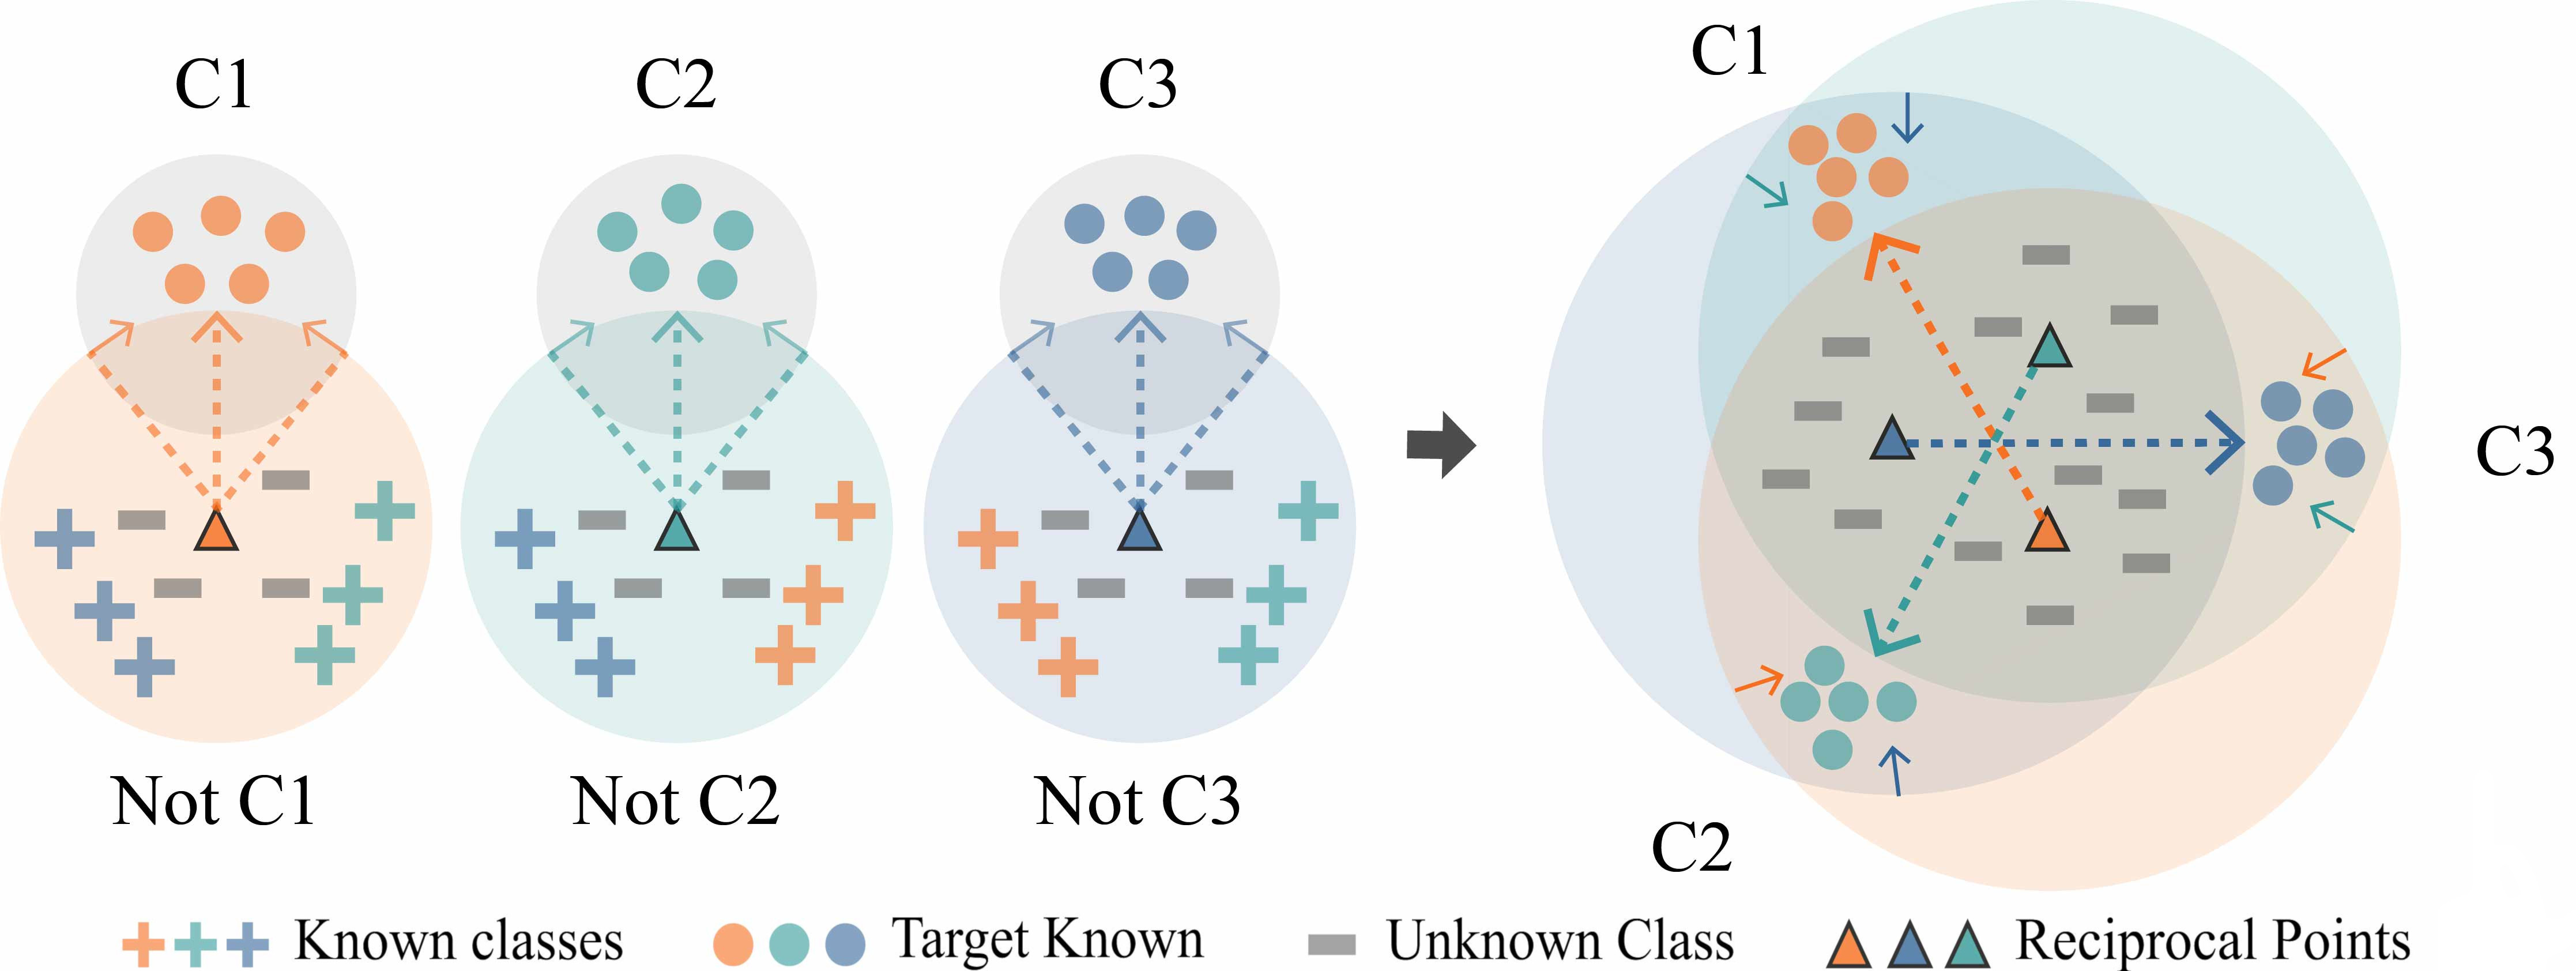
\includegraphics[width=.7\textwidth]{ARPL}
      \caption*{Reciprocal points learning scheme}
  \end{figure}
  \begin{flushright}
    \tiny{\textcolor{gray}{Chen, G., Qiao, L., Shi, Y., Peng, P., Li, J., Huang, T., Pu, S., \& Tian, Y. (2020). Learning Open Set Network with Discriminative Reciprocal Points. CoRR, abs/2011.00178. }}
  \end{flushright}
\end{frame}

\begin{frame}{Reciprocal Points Learning Method}
    \begin{definitionblock}{Definition}
        \begin{itemize}
          \item Overall loss: 
          \[
              \mathcal{L}(x; \theta, \mathcal{P}, R) = \mathcal{L}_c(x; \theta, \mathcal{P}) + \lambda \mathcal{L}_{\mathcal{O}}(x; \theta, \mathcal{P}, R)\,,
          \]
          with
          \begin{align*}
              \begin{aligned}
                  \mathcal{L}_c(x;\theta, \mathcal{P}) &= -\log p(y=k|x, f_{\theta}, \mathcal{P}) \\
                  \mathcal{L}_{\mathcal{O}}(x; \theta, \mathcal{P}^k, R^k) &= \frac{1}{M}\sum_{i=1}^M \Vert d(f_{\theta}(x), p_i^k)-R^k \Vert^2_2\,.
              \end{aligned}
          \end{align*}
        \end{itemize}
    \end{definitionblock}
\end{frame}

\begin{frame}{Perfomance Metrics}
    \begin{normalblock}{Metrics used}
        \begin{itemize}
          \item<1-> Classification metric:
          \[
              \text{accuracy} = \frac{1}{N}\sum_{i=1}^N \mathds{1} (y_i = \hat{y}_i)\,.
          \]
          \item<2-> Novelty detection: \emph{AUC} with 
          \[
              TPR = \frac{TP}{TP+FN}, \quad FPR = \frac{FP}{FP+TN}\,.
          \]
          \item<3-> Clustering: 
          \[
              ARI = \frac{R-\EX(R)}{1-\EX(R)}\,.
          \]
        \end{itemize}
    \end{normalblock}
\end{frame}

\begin{frame}{Difficulty Metric}
    \begin{definitionblock}{Definition}
        \begin{itemize}
            \item Openness: 
            \[
                \Theta = 1 - \sqrt{\frac{2|\mathcal{K}|}{2|\mathcal{K}| + |\mathcal{U}|}}\,.
            \]
        \end{itemize}
    \end{definitionblock}
\end{frame}

\section{Experiments and Results}
%\begin{frame}{Model Selection - 1}
    \noindent
    \begin{minipage}[c]{0.5\textwidth}
        \centering
        \scalebox{0.7}{
        \begin{tabular}{SSSSSSS}
            \toprule
            {\thead{\textbf{Exp.}}} & {\thead{\textbf{Architecture}}} & {\thead{\textbf{Trainable}}} & {\thead{\textbf{\#Trainable} \\ \textbf{params}}} & {\thead{\textbf{Validation} \\ \textbf{accuracy}}}\\ \midrule
            1 & {ResNet50}        & {Full}          & {23M}  & {87.8\%} \\
            2 & {EfficientNet-B1} & {Full}          & {6.5M} & {85.8\%} \\
            3 & {EfficientNet-B1} & {Final layers}  & {437K} & {80.8\%} \\ 
            4 & {EfficientNet-B4} & {Full}          & {18M}  & {87.2\%} \\ 
            5 & {EfficientNet-B4} & {Final layers}  & {832K} & {86.4\%} \\ 
            \rowcolor{Gray} 6 & {EfficientNet-B7} & {Final layers}  & {1.8M} & {89.7\%} \\ 
            \bottomrule
        \end{tabular}
        }
        \vfill
    \end{minipage}
    \hfill
    \begin{minipage}[c]{0.45\textwidth}
        \vspace*{10px}
        \centering
        \scalebox{0.5}{
            \begin{tikzpicture}[
                spy using outlines={rectangle, magnification=3, size=3cm, connect spies}]
            
                \pgfplotsset{
                    scale only axis,
                }
                
                \begin{axis}[
                    xmin=1, 
                    xmax=50, 
                    ymin=0, 
                    ymax=1,
                    grid=both,
                    grid style={gray!9, line width=.1pt},
                    legend style={font=\small, line width = 1pt, mark options={scale=2}},
                    %axis equal image
                    %x=0.4cm,
                    %y=0.4cm,
                    %ticks=none,
                    %axis background/.style={fill=gray!10},
                    legend pos = south east,
                    ylabel={Accuracy}, 
                    xlabel={Training epochs},
                    x label style={at={(axis description cs:0.5,-0.09)},anchor=north},
                    y label style={at={(axis description cs:-0.08,.5)},rotate=0, anchor=south}
                    ]
            
                    %\addlegendimage{color=red}
                    %\addlegendentry{$d_m = 1$}
            
                    \addplot[color=customred,mark =*, mark size=0.6pt] %ResNet50
                    coordinates{
                    (1,0.420)
                    (2,0.620)
                    (3,0.682)
                    (4,0.731)
                    (5,0.756)
                    (6,0.771)
                    (7,0.772)
                    (8,0.776)
                    (9,0.804)
                    (10,0.817)
                    (11,0.797)
                    (12,0.820)
                    (13,0.809)
                    (14,0.829)
                    (15,0.814)
                    (16,0.815)
                    (17,0.838)
                    (18,0.833)
                    (19,0.829)
                    (20,0.820)
                    (21,0.820)
                    (22,0.842)
                    (23,0.851)
                    (24,0.841)
                    (25,0.844)
                    (26,0.841)
                    (27,0.839)
                    (28,0.845)
                    (29,0.853)
                    (30,0.848)
                    (31,0.864)
                    (32,0.856)
                    (33,0.856)
                    (34,0.864)
                    (35,0.855)
                    (36,0.859)
                    (37,0.864)
                    (38,0.866)
                    (39,0.860)
                    (40,0.866)
                    (41,0.871)
                    (42,0.863)
                    (43,0.864)
                    (44,0.868)
                    (45,0.869)
                    (46,0.871)
                    (47,0.872)
                    (48,0.878)
                    (49,0.876)
                    (50,0.875)
                    (51,0.875)
                    (52,0.875)
                    (53,0.874)
                    (54,0.878)
                    (55,0.878)
                    (56,0.874)
                    (57,0.876)
                    (58,0.877)
                    (59,0.878)
                    (60,0.874)
                    };
            
                    \addplot[color=custompurple,mark =*, mark size=0.6pt] %ENB1 full
                    coordinates{
                    (1,0.138)
                    (2,0.438)
                    (3,0.575)
                    (4,0.586)
                    (5,0.643)
                    (6,0.630)
                    (7,0.705)
                    (8,0.675)
                    (9,0.721)
                    (10,0.747)
                    (11,0.718)
                    (12,0.716)
                    (13,0.762)
                    (14,0.772)
                    (15,0.742)
                    (16,0.764)
                    (17,0.738)
                    (18,0.759)
                    (19,0.778)
                    (20,0.755)
                    (21,0.760)
                    (22,0.745)
                    (23,0.777)
                    (24,0.777)
                    (25,0.781)
                    (26,0.795)
                    (27,0.797)
                    (28,0.807)
                    (29,0.800)
                    (30,0.812)
                    (31,0.822)
                    (32,0.815)
                    (33,0.803)
                    (34,0.807)
                    (35,0.832)
                    (36,0.826)
                    (37,0.828)
                    (38,0.834)
                    (39,0.816)
                    (40,0.837)
                    (41,0.839)
                    (42,0.832)
                    (43,0.833)
                    (44,0.843)
                    (45,0.849)
                    (46,0.838)
                    (47,0.849)
                    (48,0.844)
                    (49,0.852)
                    (50,0.851)
                    (51,0.852)
                    (52,0.844)
                    (53,0.851)
                    (54,0.845)
                    (55,0.861)
                    (56,0.850)
                    (57,0.851)
                    (58,0.848)
                    (59,0.851)
                    (60,0.858)
                    };
            
                    \addplot[color=customorange, mark =*, mark size=0.6pt] %ENB1 final
                    coordinates{
                    (1,0.652)
                    (2,0.673)
                    (3,0.690)
                    (4,0.739)
                    (5,0.685)
                    (6,0.741)
                    (7,0.753)
                    (8,0.746)
                    (9,0.717)
                    (10,0.740)
                    (11,0.719)
                    (12,0.735)
                    (13,0.762)
                    (14,0.774)
                    (15,0.771)
                    (16,0.740)
                    (17,0.758)
                    (18,0.757)
                    (19,0.750)
                    (20,0.773)
                    (21,0.767)
                    (22,0.772)
                    (23,0.771)
                    (24,0.749)
                    (25,0.759)
                    (26,0.769)
                    (27,0.781)
                    (28,0.779)
                    (29,0.773)
                    (30,0.781)
                    (31,0.779)
                    (32,0.765)
                    (33,0.783)
                    (34,0.771)
                    (35,0.781)
                    (36,0.772)
                    (37,0.774)
                    (38,0.794)
                    (39,0.777)
                    (40,0.792)
                    (41,0.788)
                    (42,0.795)
                    (43,0.792)
                    (44,0.794)
                    (45,0.801)
                    (46,0.788)
                    (47,0.799)
                    (48,0.780)
                    (49,0.800)
                    (50,0.798)
                    (51,0.798)
                    (52,0.804)
                    (53,0.801)
                    (54,0.798)
                    (55,0.807)
                    (56,0.807)
                    (57,0.795)
                    (58,0.798)
                    (59,0.804)
                    (60,0.803)
                    };
            
                    \addplot[color = customblue, mark =*, mark size=0.6pt] %ENB4-full
                    coordinates{
                    (1,0.327)
                    (2,0.368)
                    (3,0.568)
                    (4,0.559)
                    (5,0.669)
                    (6,0.642)
                    (7,0.606)
                    (8,0.688)
                    (9,0.712)
                    (10,0.706)
                    (11,0.714)
                    (12,0.752)
                    (13,0.736)
                    (14,0.722)
                    (15,0.775)
                    (16,0.688)
                    (17,0.774)
                    (18,0.777)
                    (19,0.767)
                    (20,0.775)
                    (21,0.814)
                    (22,0.818)
                    (23,0.801)
                    (24,0.795)
                    (25,0.793)
                    (26,0.824)
                    (27,0.821)
                    (28,0.814)
                    (29,0.828)
                    (30,0.821)
                    (31,0.823)
                    (32,0.822)
                    (33,0.819)
                    (34,0.813)
                    (35,0.839)
                    (36,0.827)
                    (37,0.828)
                    (38,0.836)
                    (39,0.843)
                    (40,0.837)
                    (41,0.849)
                    (42,0.850)
                    (43,0.841)
                    (44,0.859)
                    (45,0.842)
                    (46,0.853)
                    (47,0.860)
                    (48,0.862)
                    (49,0.861)
                    (50,0.854)
                    (51,0.861)
                    (52,0.857)
                    (53,0.862)
                    (54,0.861)
                    (55,0.861)
                    (56,0.865)
                    (57,0.864)
                    (58,0.867)
                    (59,0.872)
                    (60,0.870)
                    };
            
                    \addplot[color = custommagenta, mark =*, mark size=0.6pt] %ENB4 final
                    coordinates{
                    (1,0.700)
                    (2,0.742)
                    (3,0.773)
                    (4,0.781)
                    (5,0.791)
                    (6,0.783)
                    (7,0.781)
                    (8,0.796)
                    (9,0.805)
                    (10,0.816)
                    (11,0.818)
                    (12,0.807)
                    (13,0.819)
                    (14,0.834)
                    (15,0.819)
                    (16,0.827)
                    (17,0.828)
                    (18,0.830)
                    (19,0.831)
                    (20,0.831)
                    (21,0.847)
                    (22,0.837)
                    (23,0.836)
                    (24,0.841)
                    (25,0.827)
                    (26,0.824)
                    (27,0.844)
                    (28,0.838)
                    (29,0.841)
                    (30,0.841)
                    (31,0.844)
                    (32,0.838)
                    (33,0.837)
                    (34,0.846)
                    (35,0.846)
                    (36,0.834)
                    (37,0.854)
                    (38,0.843)
                    (39,0.850)
                    (40,0.841)
                    (41,0.855)
                    (42,0.848)
                    (43,0.851)
                    (44,0.855)
                    (45,0.848)
                    (46,0.851)
                    (47,0.848)
                    (48,0.856)
                    (49,0.856)
                    (50,0.853)
                    (51,0.861)
                    (52,0.860)
                    (53,0.859)
                    (54,0.855)
                    (55,0.855)
                    (56,0.858)
                    (57,0.864)
                    (58,0.863)
                    (59,0.861)
                    (60,0.857)
                    };
            
                    \addplot[color = customgreen, mark =*, mark size=0.6pt] %ENB7 final
                    coordinates{
                    (1,0.679)
                    (2,0.810)
                    (3,0.833)
                    (4,0.803)
                    (5,0.829)
                    (6,0.825)
                    (7,0.849)
                    (8,0.859)
                    (9,0.863)
                    (10,0.854)
                    (11,0.838)
                    (12,0.870)
                    (13,0.867)
                    (14,0.875)
                    (15,0.871)
                    (16,0.864)
                    (17,0.864)
                    (18,0.870)
                    (19,0.875)
                    (20,0.886)
                    (21,0.875)
                    (22,0.871)
                    (23,0.879)
                    (24,0.880)
                    (25,0.881)
                    (26,0.882)
                    (27,0.876)
                    (28,0.890)
                    (29,0.886)
                    (30,0.884)
                    (31,0.889)
                    (32,0.887)
                    (33,0.885)
                    (34,0.891)
                    (35,0.894)
                    (36,0.890)
                    (37,0.894)
                    (38,0.897)
                    (39,0.887)
                    (40,0.892)
                    (41,0.894)
                    (42,0.888)
                    (43,0.887)
                    (44,0.888)
                    (45,0.892)
                    (46,0.886)
                    (47,0.893)
                    (48,0.896)
                    (49,0.891)
                    (50,0.885)
                    (51,0.892)
                    (52,0.894)
                    (53,0.889)
                    (54,0.895)
                    (55,0.898)
                    (56,0.897)
                    (57,0.900)
                    (58,0.899)
                    (59,0.899)
                    (60,0.897)
                    };
                    \legend{ResNet50/Full,
                            EfficientNet-B1/Full,
                            EfficientNet-B1/Final,
                            EfficientNet-B4/Full,
                            EfficientNet-B1/Final,
                            EfficientNet-B7/Final,}
            
                    \spy [black] on (7.93,6.15) in node at (10,3.5);
                    
                \end{axis}
            \end{tikzpicture}
            }
    \end{minipage}
\end{frame}

\begin{frame}{Model Selection - 2}
    \noindent
    \begin{minipage}[c]{0.5\textwidth}
        \centering
        \scalebox{0.63}{
        \begin{tabular}{SSSSSSSS}
            \toprule
            {\thead{\textbf{Exp.}}} & {\thead{\textbf{Architecture}}} & {\thead{\textbf{Trainable}}} & {\thead{\textbf{Label} \\ \textbf{smoothing}}} & {\thead{$\bm{\eta}$}} & {\thead{\textbf{Batch} \\ \textbf{size}}} & {\thead{\textbf{Validation} \\ \textbf{accuracy}}}\\ \midrule
            0 & {EfficientNet-B7} & {Final layers}  & {0}   & {0.01}   & {4}  & {89.7\%}\\ %run14 
            \midrule
            1 & {EfficientNet-B7} & {Final layers}  & {0.1} & {0.01}   & {4}  & {79.5\%}\\ %run15
            2 & {EfficientNet-B7} & {Final layers}  & {0.01}& {0.01}   & {4}  & {88.5\%}\\ %run16
            3 & {EfficientNet-B7} & {Final layers}  & {0}   & {0.01}   & {2}  & {77.7\%}\\ %run20 
            4 & {EfficientNet-B7} & {Final layers}  & {0}   & {0.001}  & {2}  & {81.1\%}\\ %run22
            \rowcolor{Gray} 5 & {EfficientNet-B7} & {Final layers}  & {0}   & {0.01}   & {8}  & {92.8\%}\\ %run24
            6 & {EfficientNet-B7} & {Final layers}  & {0}   & {0.1}    & {16} & {91.7\%}\\ %run25
            7 & {EfficientNet-B7} & {Final layers}  & {0}   & {0.1}    & {32} & {91.4\%}\\ %run26
            8 & {EfficientNet-B7} & {Final layers}  & {0}   & {0.1}    & {64} & {92.7\%}\\ %run27
            \bottomrule
        \end{tabular}
        }
    \end{minipage}
    \hfill
    \begin{minipage}[c]{0.45\textwidth}
        \vspace*{10px}
        \centering
        \scalebox{0.5}{
        \begin{tikzpicture}[
            spy using outlines={rectangle, magnification=3, size=3cm, connect spies}]
            
                \pgfplotsset{
                    scale only axis,
                }
                
                \begin{axis}[
                xmin=1, 
                xmax=60, 
                ymin=0, 
                ymax=1,
                grid=both,
                grid style={gray!9, line width=.1pt},
                %axis equal image
                %x=0.4cm,
                %y=0.4cm,
                %ticks=none,
                %axis background/.style={fill=gray!10},
                legend style={font=\tiny, line width = 1pt, mark options={scale=2}},
                legend pos = south east,
                ylabel={Accuracy}, 
                xlabel={Training epochs},
                x label style={at={(axis description cs:0.5,-0.09)},anchor=north},
                y label style={at={(axis description cs:-0.08,.5)},rotate=0, anchor=south},
                ]
        
                %\addlegendimage{color=red}
                %\addlegendentry{$d_m = 1$}
        
                \addplot[color=customred,mark =*, mark size=0.6pt] %run14
                coordinates{
                    (1,0.679)
        (2,0.810)
        (3,0.833)
        (4,0.803)
        (5,0.829)
        (6,0.825)
        (7,0.849)
        (8,0.859)
        (9,0.863)
        (10,0.854)
        (11,0.838)
        (12,0.870)
        (13,0.867)
        (14,0.875)
        (15,0.871)
        (16,0.864)
        (17,0.864)
        (18,0.870)
        (19,0.875)
        (20,0.886)
        (21,0.875)
        (22,0.871)
        (23,0.879)
        (24,0.880)
        (25,0.881)
        (26,0.882)
        (27,0.876)
        (28,0.890)
        (29,0.886)
        (30,0.884)
        (31,0.889)
        (32,0.887)
        (33,0.885)
        (34,0.891)
        (35,0.894)
        (36,0.890)
        (37,0.894)
        (38,0.897)
        (39,0.887)
        (40,0.892)
        (41,0.894)
        (42,0.888)
        (43,0.887)
        (44,0.888)
        (45,0.892)
        (46,0.886)
        (47,0.893)
        (48,0.896)
        (49,0.891)
        (50,0.885)
        (51,0.892)
        (52,0.894)
        (53,0.889)
        (54,0.895)
        (55,0.898)
        (56,0.897)
        (57,0.900)
        (58,0.899)
        (59,0.899)
        (60,0.897)
                };
        
                \addplot[color=customred,mark =triangle, mark size=1.2pt] %run15
                coordinates{
                    (1,0.731)
        (2,0.730)
        (3,0.735)
        (4,0.779)
        (5,0.802)
        (6,0.850)
        (7,0.826)
        (8,0.856)
        (9,0.841)
        (10,0.842)
        (11,0.859)
        (12,0.853)
        (13,0.851)
        (14,0.855)
        (15,0.848)
        (16,0.838)
        (17,0.846)
        (18,0.838)
        (19,0.827)
        (20,0.815)
        (21,0.834)
        (22,0.826)
        (23,0.829)
        (24,0.831)
        (25,0.791)
        (26,0.816)
        (27,0.808)
        (28,0.803)
        (29,0.803)
        (30,0.803)
        (31,0.777)
        (32,0.796)
        (33,0.803)
        (34,0.800)
        (35,0.813)
        (36,0.796)
        (37,0.817)
        (38,0.810)
        (39,0.795)
                };
        
                \addplot[color=customred,mark =x, mark size=1pt] %run16
                coordinates{
                    (1,0.756)
        (2,0.794)
        (3,0.818)
        (4,0.828)
        (5,0.824)
        (6,0.843)
        (7,0.857)
        (8,0.856)
        (9,0.858)
        (10,0.849)
        (11,0.859)
        (12,0.857)
        (13,0.868)
        (14,0.872)
        (15,0.866)
        (16,0.868)
        (17,0.872)
        (18,0.863)
        (19,0.875)
        (20,0.858)
        (21,0.870)
        (22,0.881)
        (23,0.862)
        (24,0.882)
        (25,0.874)
        (26,0.874)
        (27,0.873)
        (28,0.877)
        (29,0.885)
        (30,0.879)
        (31,0.887)
        (32,0.891)
        (33,0.884)
        (34,0.882)
        (35,0.889)
        (36,0.879)
        (37,0.884)
        (38,0.884)
        (39,0.886)
        (40,0.886)
        (41,0.882)
        (42,0.889)
        (43,0.889)
        (44,0.890)
        (45,0.880)
        (46,0.877)
        (47,0.886)
        (48,0.889)
        (49,0.891)
        (50,0.884)
        (51,0.888)
        (52,0.886)
        (53,0.888)
        (54,0.884)
        (55,0.893)
        (56,0.891)
        (57,0.888)
        (58,0.888)
        (59,0.889)
        (60,0.885)
                };
        
                \addplot[color=custompurple,mark =*, mark size=0.6pt] %run20
                coordinates{
                    (1,0.563)
        (2,0.667)
        (3,0.686)
        (4,0.652)
        (5,0.696)
        (6,0.674)
        (7,0.673)
        (8,0.666)
        (9,0.654)
        (10,0.718)
        (11,0.734)
        (12,0.684)
        (13,0.714)
        (14,0.711)
        (15,0.725)
        (16,0.706)
        (17,0.729)
        (18,0.732)
        (19,0.733)
        (20,0.745)
        (21,0.728)
        (22,0.745)
        (23,0.730)
        (24,0.714)
        (25,0.754)
        (26,0.749)
        (27,0.745)
        (28,0.742)
        (29,0.755)
        (30,0.743)
        (31,0.733)
        (32,0.751)
        (33,0.753)
        (34,0.737)
        (35,0.748)
        (36,0.750)
        (37,0.745)
        (38,0.775)
        (39,0.745)
        (40,0.748)
        (41,0.745)
        (42,0.756)
        (43,0.765)
        (44,0.770)
        (45,0.756)
        (46,0.767)
        (47,0.748)
        (48,0.786)
        (49,0.746)
        (50,0.767)
        (51,0.778)
        (52,0.788)
        (53,0.770)
        (54,0.777)
        (55,0.775)
        (56,0.762)
        (57,0.788)
        (58,0.775)
        (59,0.772)
        (60,0.761)
                };
        
                \addplot[color=custompurple, mark =triangle, mark size=1.2pt] %run22
                coordinates{
                    (1,0.650)
        (2,0.638)
        (3,0.707)
        (4,0.695)
        (5,0.713)
        (6,0.723)
        (7,0.726)
        (8,0.732)
        (9,0.722)
        (10,0.750)
        (11,0.741)
        (12,0.764)
        (13,0.739)
        (14,0.764)
        (15,0.756)
        (16,0.731)
        (17,0.772)
        (18,0.745)
        (19,0.760)
        (20,0.750)
        (21,0.739)
        (22,0.744)
        (23,0.745)
        (24,0.755)
        (25,0.769)
        (26,0.778)
        (27,0.780)
        (28,0.790)
        (29,0.770)
        (30,0.766)
        (31,0.780)
        (32,0.769)
        (33,0.769)
        (34,0.790)
        (35,0.771)
        (36,0.772)
        (37,0.779)
        (38,0.773)
        (39,0.755)
        (40,0.793)
        (41,0.782)
        (42,0.776)
        (43,0.784)
        (44,0.791)
        (45,0.788)
        (46,0.790)
        (47,0.789)
        (48,0.786)
        (49,0.772)
        (50,0.787)
        (51,0.798)
        (52,0.796)
        (53,0.790)
        (54,0.785)
        (55,0.781)
        (56,0.800)
        (57,0.802)
        (58,0.793)
        (59,0.805)
        (60,0.811)
                };
        
                \addplot[color = customblue, mark =*, mark size=0.6pt] %run24
                coordinates{
                    (1,0.776)
        (2,0.848)
        (3,0.836)
        (4,0.841)
        (5,0.878)
        (6,0.879)
        (7,0.877)
        (8,0.883)
        (9,0.886)
        (10,0.871)
        (11,0.894)
        (12,0.898)
        (13,0.886)
        (14,0.893)
        (15,0.895)
        (16,0.901)
        (17,0.894)
        (18,0.896)
        (19,0.908)
        (20,0.902)
        (21,0.909)
        (22,0.896)
        (23,0.898)
        (24,0.903)
        (25,0.908)
        (26,0.904)
        (27,0.898)
        (28,0.905)
        (29,0.910)
        (30,0.916)
        (31,0.906)
        (32,0.913)
        (33,0.915)
        (34,0.905)
        (35,0.918)
        (36,0.912)
        (37,0.919)
        (38,0.914)
        (39,0.919)
        (40,0.922)
        (41,0.916)
        (42,0.915)
        (43,0.916)
        (44,0.924)
        (45,0.909)
        (46,0.916)
        (47,0.921)
        (48,0.919)
        (49,0.925)
        (50,0.921)
        (51,0.925)
        (52,0.926)
        (53,0.922)
        (54,0.922)
        (55,0.920)
        (56,0.924)
        (57,0.926)
        (58,0.922)
        (59,0.919)
        (60,0.928)
                };
        
                \addplot[color = customblack, mark =*, mark size=0.6pt] %run25
                coordinates{
                    (1,0.779)
        (2,0.806)
        (3,0.769)
        (4,0.825)
        (5,0.800)
        (6,0.826)
        (7,0.835)
        (8,0.835)
        (9,0.835)
        (10,0.841)
        (11,0.832)
        (12,0.850)
        (13,0.849)
        (14,0.867)
        (15,0.843)
        (16,0.871)
        (17,0.872)
        (18,0.876)
        (19,0.860)
        (20,0.866)
        (21,0.877)
        (22,0.869)
        (23,0.857)
        (24,0.869)
        (25,0.890)
        (26,0.877)
        (27,0.880)
        (28,0.885)
        (29,0.875)
        (30,0.880)
        (31,0.894)
        (32,0.887)
        (33,0.883)
        (34,0.880)
        (35,0.878)
        (36,0.899)
        (37,0.895)
        (38,0.892)
        (39,0.901)
        (40,0.897)
        (41,0.900)
        (42,0.899)
        (43,0.902)
        (44,0.904)
        (45,0.906)
        (46,0.914)
        (47,0.901)
        (48,0.903)
        (49,0.907)
        (50,0.910)
        (51,0.907)
        (52,0.906)
        (53,0.909)
        (54,0.905)
        (55,0.904)
        (56,0.905)
        (57,0.915)
        (58,0.910)
        (59,0.906)
        (60,0.917)
                };
        
                \addplot[color = customgreen, mark =*, mark size=0.6pt] %run26
                coordinates{
                    (1,0.800)
        (2,0.826)
        (3,0.861)
        (4,0.867)
        (5,0.850)
        (6,0.850)
        (7,0.856)
        (8,0.862)
        (9,0.861)
        (10,0.843)
        (11,0.880)
        (12,0.863)
        (13,0.881)
        (14,0.865)
        (15,0.878)
        (16,0.867)
        (17,0.887)
        (18,0.883)
        (19,0.887)
        (20,0.894)
        (21,0.890)
        (22,0.892)
        (23,0.892)
        (24,0.897)
        (25,0.896)
        (26,0.893)
        (27,0.875)
        (28,0.891)
        (29,0.897)
        (30,0.894)
        (31,0.898)
        (32,0.898)
        (33,0.900)
        (34,0.904)
        (35,0.907)
        (36,0.909)
        (37,0.905)
        (38,0.900)
        (39,0.902)
        (40,0.903)
        (41,0.899)
        (42,0.902)
        (43,0.904)
        (44,0.903)
        (45,0.911)
        (46,0.913)
        (47,0.912)
        (48,0.909)
        (49,0.908)
        (50,0.916)
        (51,0.911)
        (52,0.915)
        (53,0.913)
        (54,0.912)
        (55,0.916)
        (56,0.908)
        (57,0.914)
        (58,0.913)
        (59,0.914)
        (60,0.914)
                };
        
                \addplot[color = custommagenta, mark =*, mark size=0.6pt] %run27
                coordinates{
                    (1,0.790)
        (2,0.835)
        (3,0.856)
        (4,0.886)
        (5,0.882)
        (6,0.861)
        (7,0.885)
        (8,0.869)
        (9,0.881)
        (10,0.879)
        (11,0.888)
        (12,0.890)
        (13,0.895)
        (14,0.876)
        (15,0.894)
        (16,0.900)
        (17,0.896)
        (18,0.893)
        (19,0.894)
        (20,0.897)
        (21,0.901)
        (22,0.899)
        (23,0.899)
        (24,0.907)
        (25,0.898)
        (26,0.900)
        (27,0.898)
        (28,0.905)
        (29,0.896)
        (30,0.903)
        (31,0.910)
        (32,0.903)
        (33,0.914)
        (34,0.917)
        (35,0.908)
        (36,0.901)
        (37,0.916)
        (38,0.911)
        (39,0.915)
        (40,0.916)
        (41,0.915)
        (42,0.919)
        (43,0.920)
        (44,0.914)
        (45,0.918)
        (46,0.922)
        (47,0.927)
        (48,0.922)
        (49,0.924)
        (50,0.931)
        (51,0.924)
        (52,0.921)
        (53,0.923)
        (54,0.924)
        (55,0.923)
        (56,0.926)
        (57,0.922)
        (58,0.923)
        (59,0.928)
        (60,0.928)
                };
                \legend{0,1,2,3,4,5,6,7,8}
        
                \spy [black] on (7.93,6.5) in node at (10,3.5);
                
                \end{axis}
        \end{tikzpicture}
        }
    \end{minipage}
\end{frame}

\begin{frame}{Clustering Algorithm Selection}
    \begin{minipage}{0.3\textwidth}
        \centering
        \scalebox{0.75}{
            \begin{tabular}{SSS}
            \toprule
            {\thead{\textbf{Exp.}}} & {\thead{\textbf{Clustering} \\ \textbf{algorithm}}} & {\thead{\textbf{ARI}}} \\ \midrule
            \rowcolor{Gray} 1 & {Gaussian Mixtures}    & {0.342} \\ 
            2 & {K-Means}              & {0.285} \\ 
            3 & {Fuzzy K-Means}        & {0.259} \\ 
            4 & {Spectral clustering}  & {0.260} \\ 
            5 & {Mean-Shift}           & {0.035} \\ 
            6 & {OPTICS}               & {0.080} \\ 
            7 & {BIRCH}                & {0.335} \\ 
            8 & {DBSCAN}               & {0.337} \\ 
            9 & {Affinity propagation} & {0.308} \\
            \bottomrule
            \end{tabular}
        }
    \end{minipage}
    \hfill
    \begin{minipage}{0.65\textwidth}
        \vspace*{10px}
        \begin{figure}
            \begin{subfigure}{.45\textwidth}
                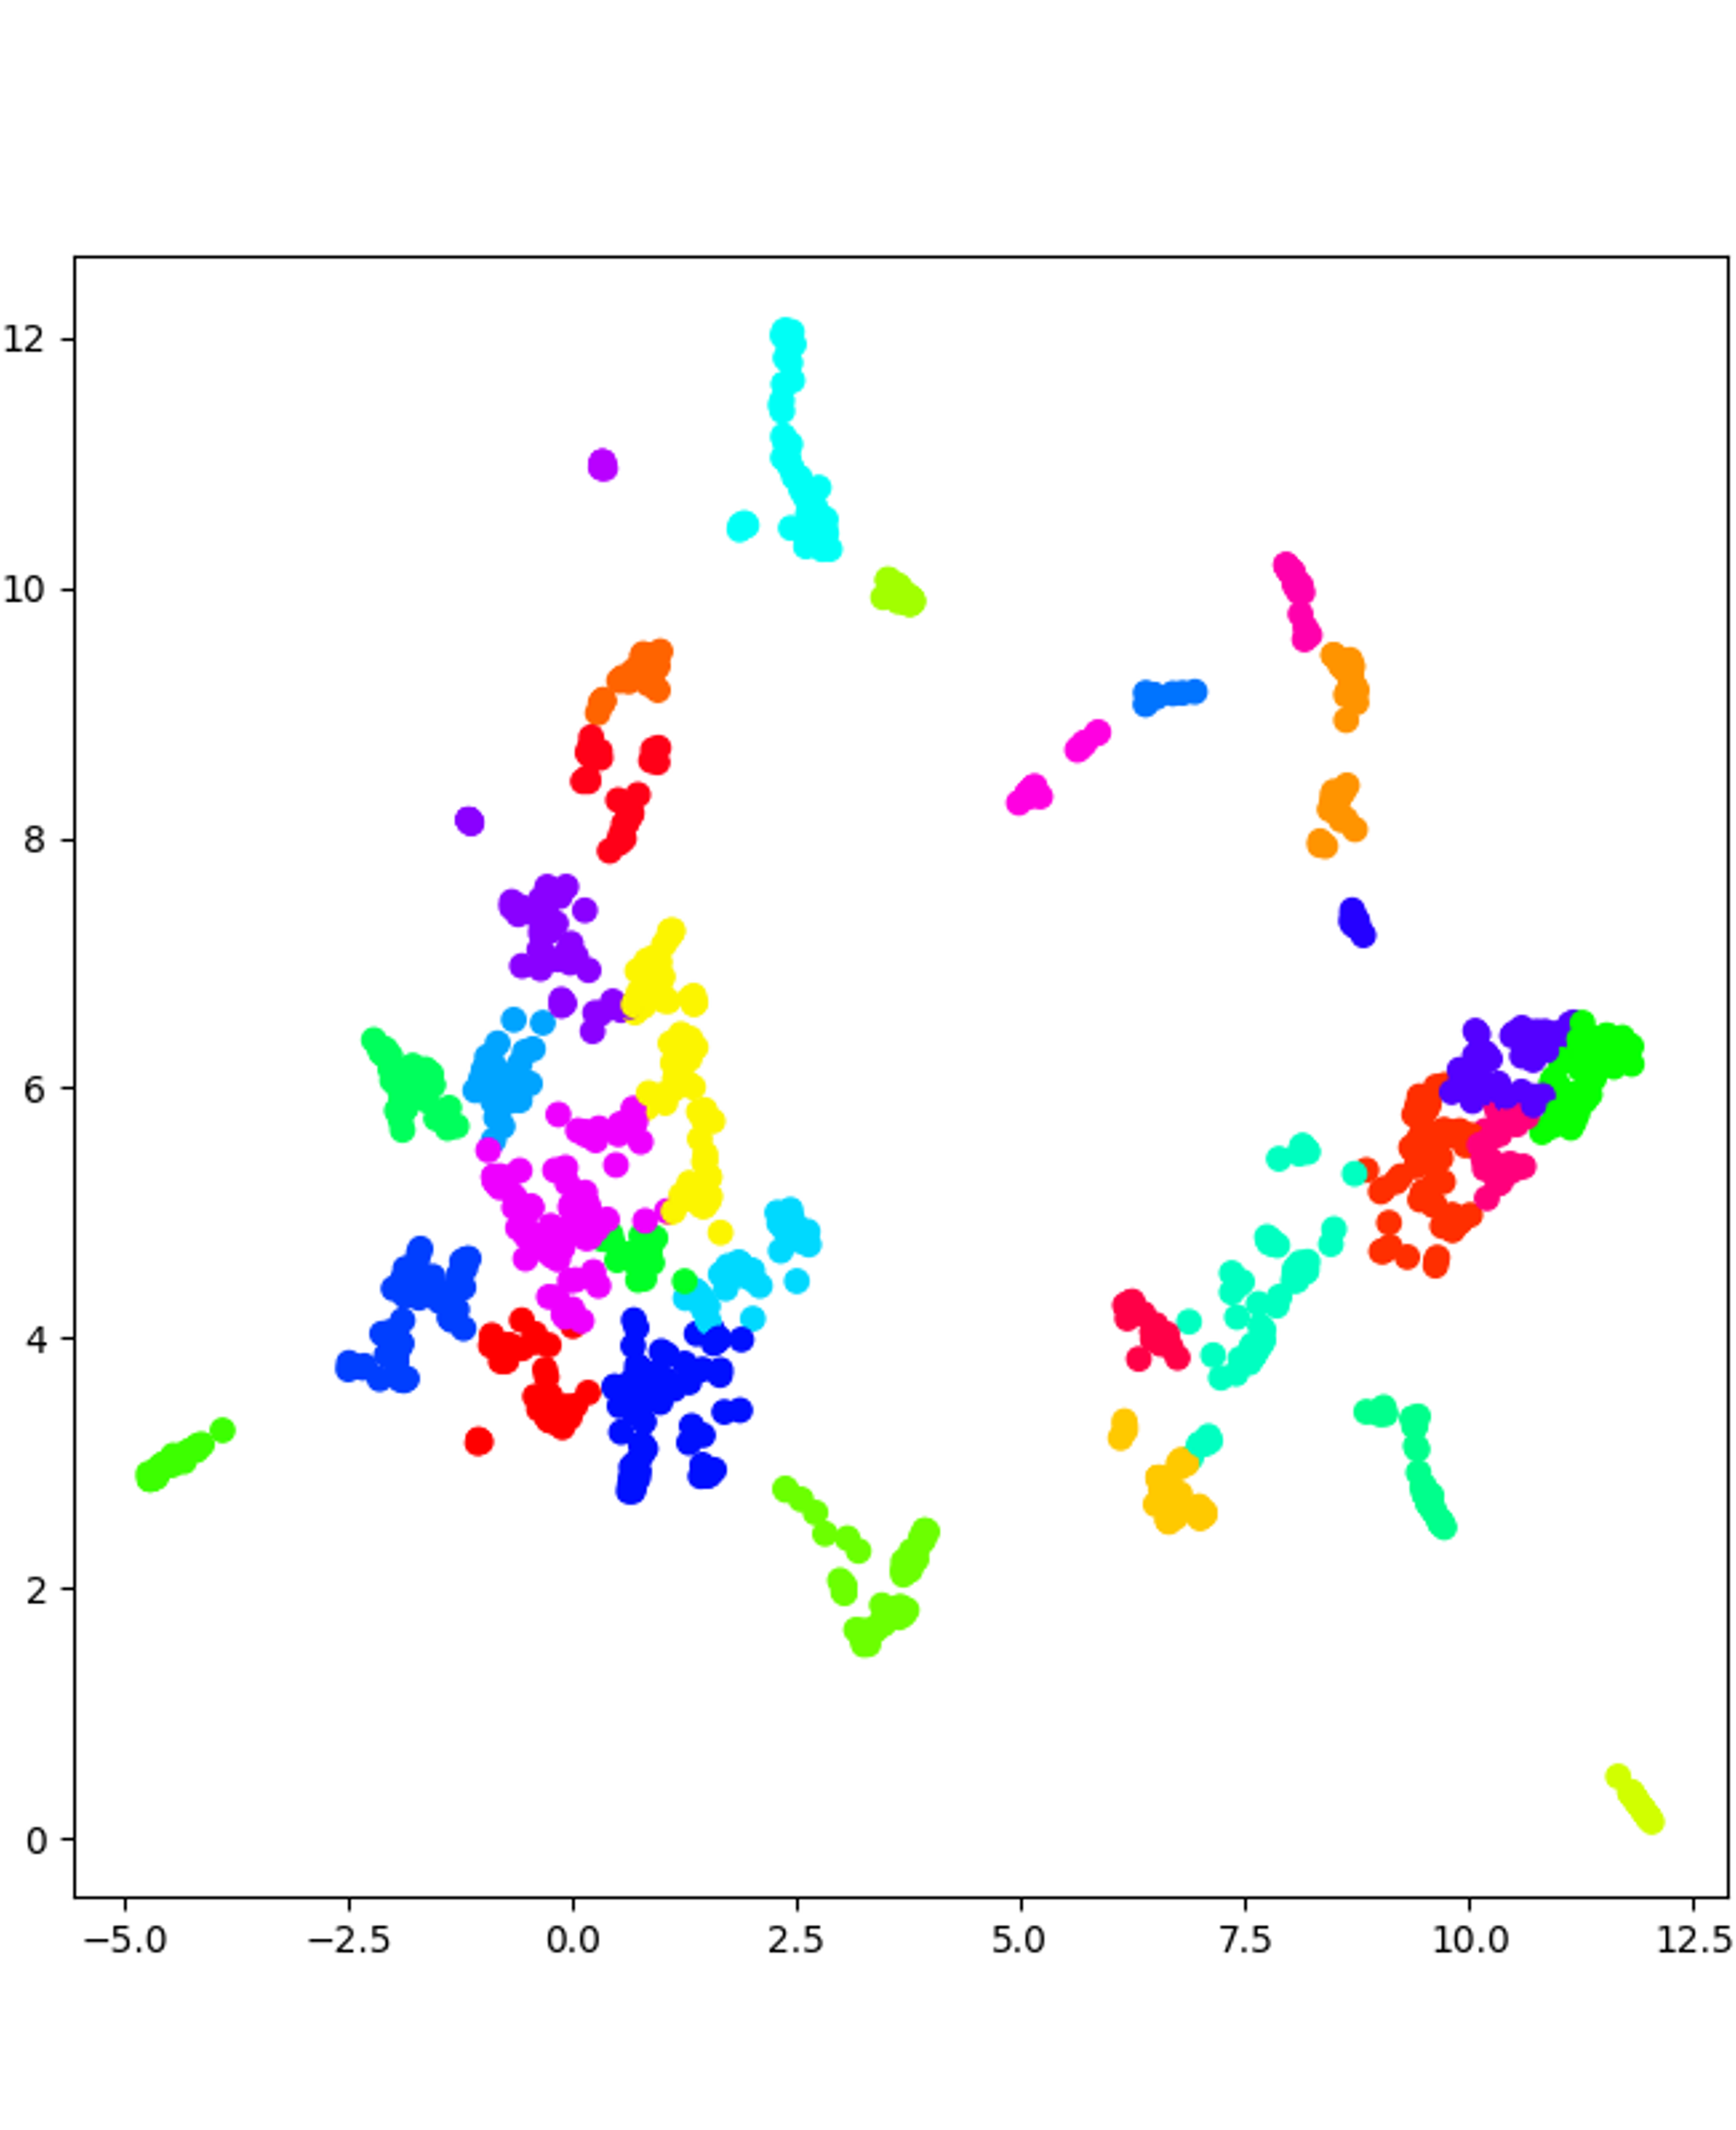
\includegraphics[width=\textwidth]{clust_pred}
                \subcaption*{\,\,\, Predicted clusters (GMM)}
            \end{subfigure}%
            \begin{subfigure}{.45\textwidth}
                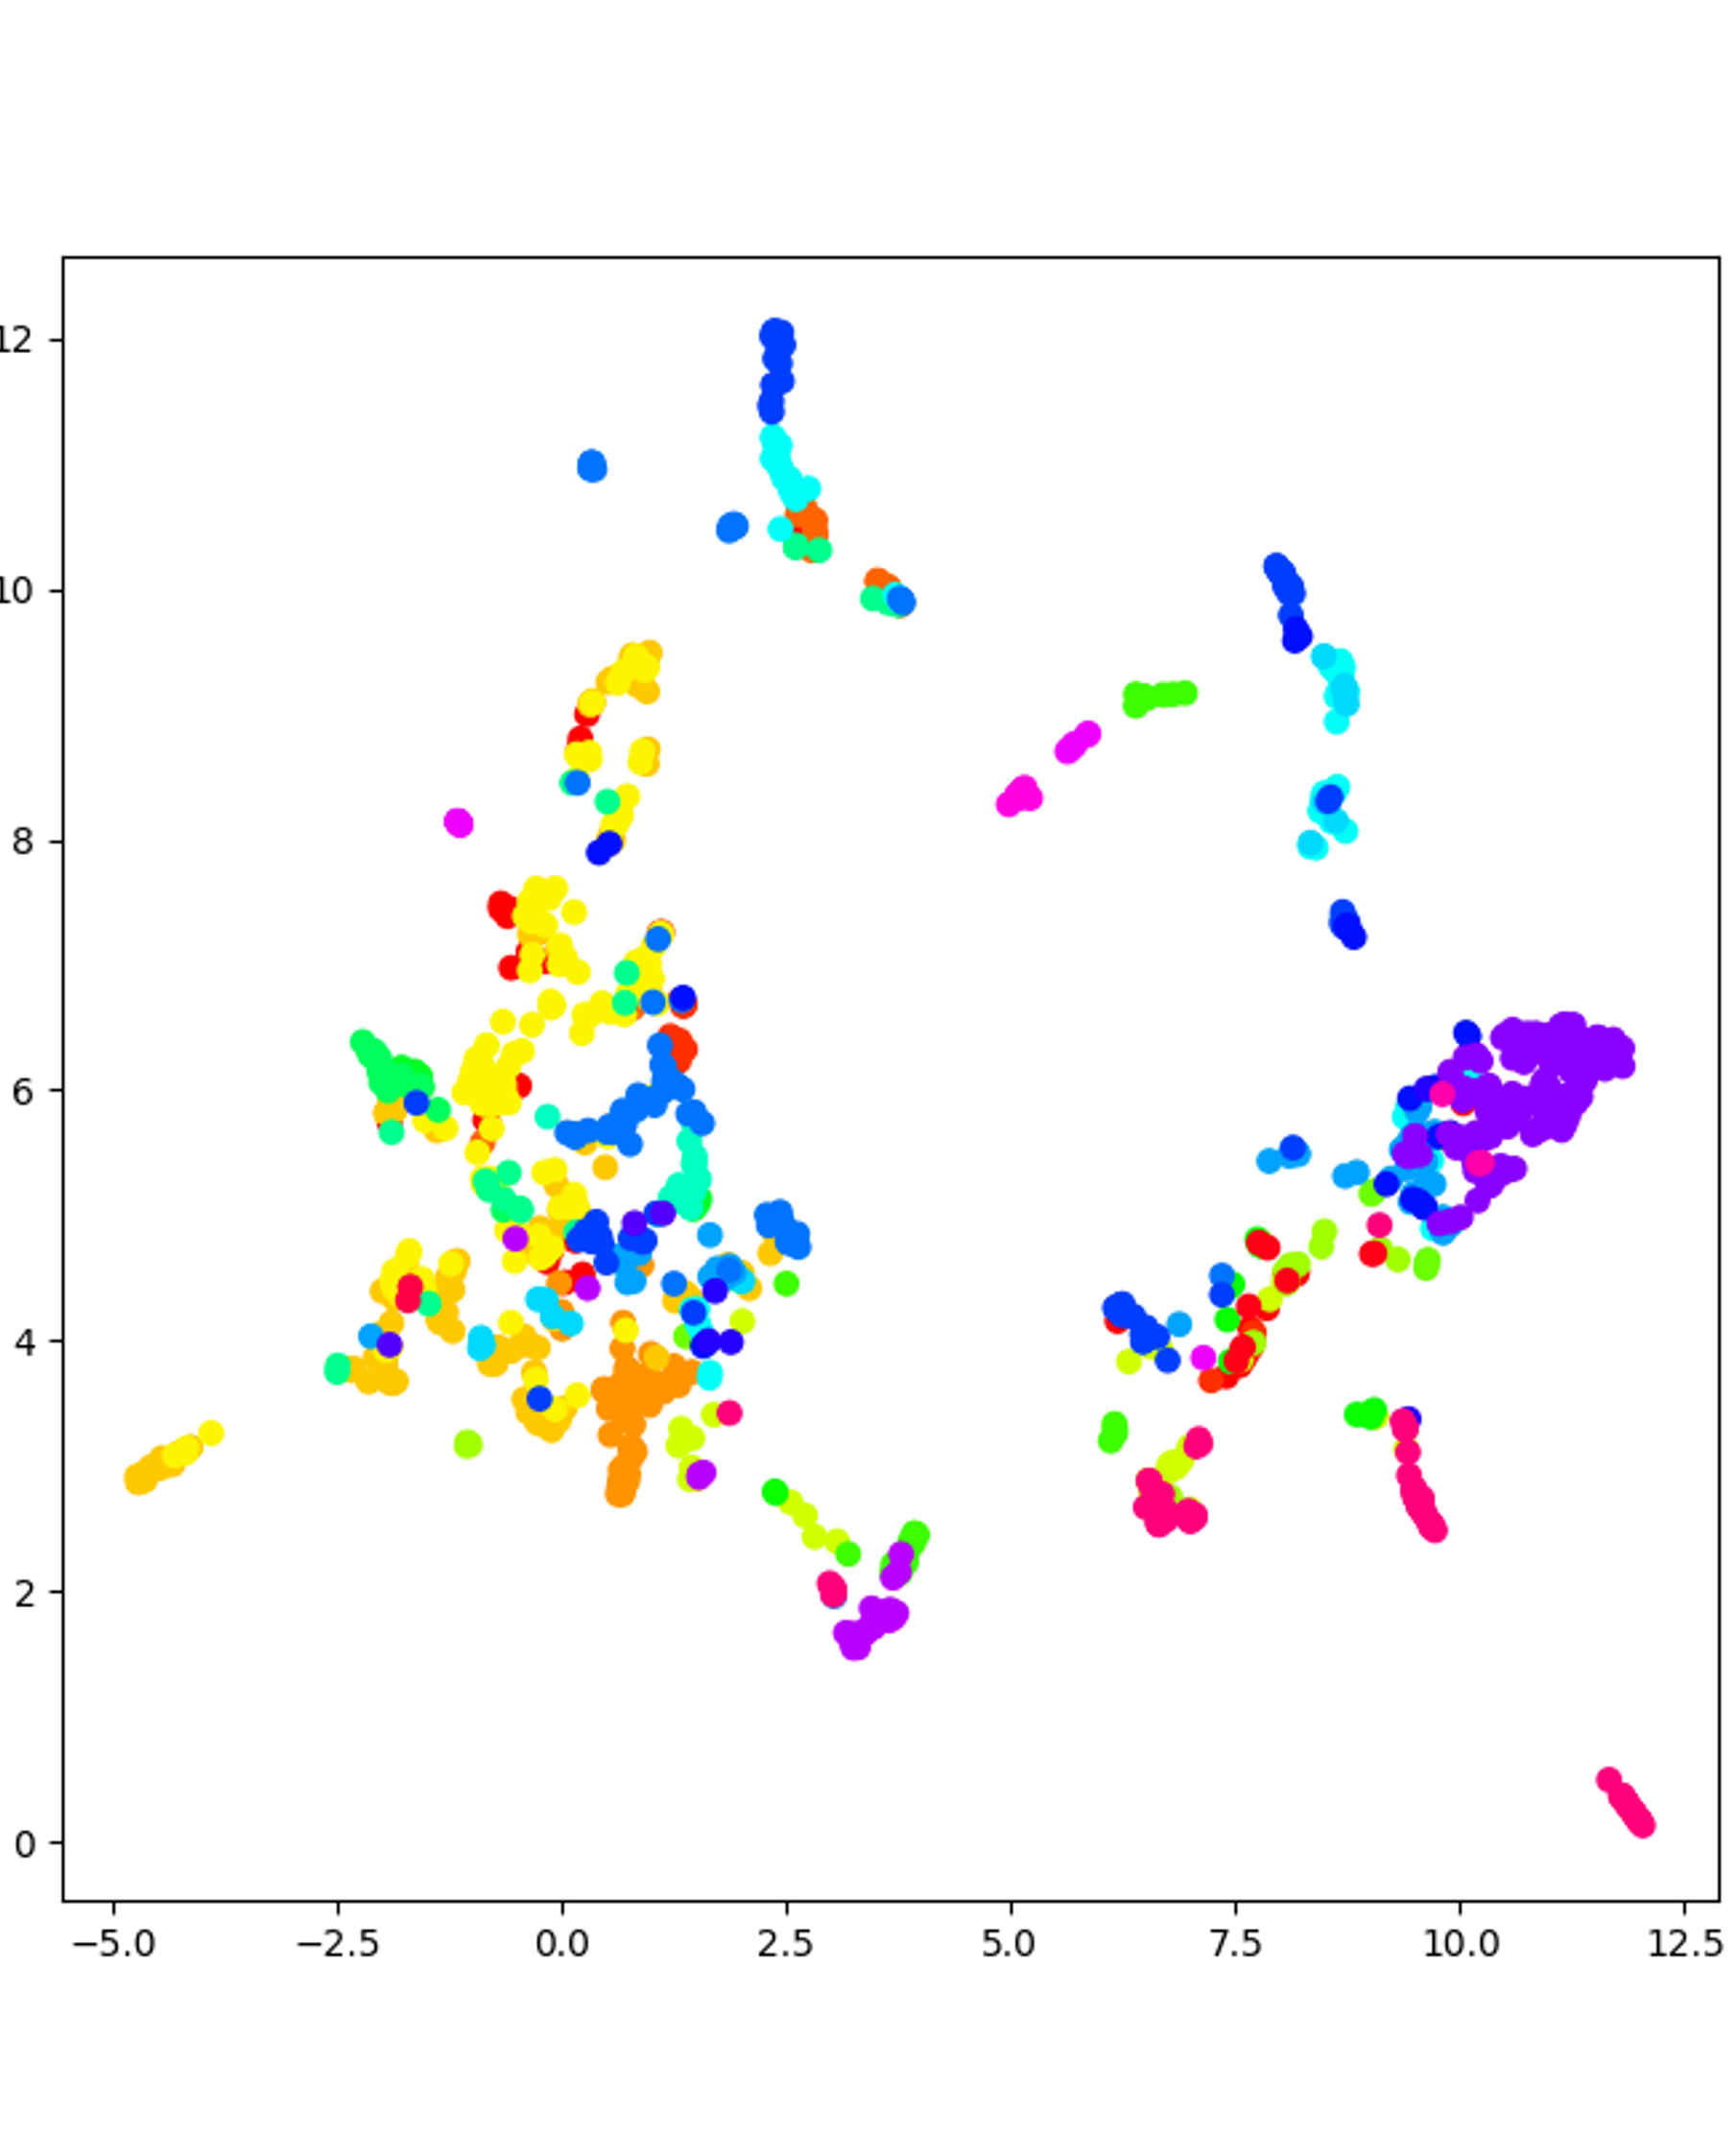
\includegraphics[width=\textwidth]{clust_truth}
                \subcaption*{\,\,\, Real clusters}
            \end{subfigure}
        \end{figure}
    \end{minipage}
\end{frame}

\begin{frame}{Dataset Setups}
    \begin{table}[]
        \centering
        \begin{tabular}{SSSSS}
        \toprule
        {\thead{\textbf{Setup}}} & {\thead{$\bm{\Theta}$}} & {\thead{\textbf{\#Knowns}}} & {\thead{\textbf{\#Unknowns}}} & {\thead{\textbf{\#Variations}}}\\ \midrule
        1 & {1.0\%}    & 36 & 1  & 7 \\ 
        2 & {4.6\%}  & 5  & 1  & 7 \\ 
        3 & {8.2\%}  & 27 & 10 & 1 \\
        4 & {20.1\%} & 17 & 20 & 1 \\ \bottomrule
        \end{tabular}
        \caption*{List of setups used for OSR experiments}
    \end{table}
\end{frame}

\begin{frame}{OSR Results}
    \begin{overprint}
        \onslide<1>\begin{table}[h]
            \centering
            \begin{tabular}{c|cc|ccccc}
                \toprule
                & & &  \multicolumn{3}{S}{\textbf{Distance method}} & \multicolumn{2}{S}{\textbf{RPL method}} \\ \midrule
                & {\textbf{Setup}} & {$\bm{\Theta}$} &  {\textbf{Accuracy}} & {\textbf{AUC-1}} & {\textbf{AUC-2}} &  {\textbf{Accuracy}} & {\textbf{AUC}} \\ \midrule
                \multirow{4}*{\rotatebox[origin=S]{90}{\textbf{RN50}}} & {1} & {1.0\%}    & {89.9\%}   & {0.64} & {0.52} & {85.6\%}    & {0.80} \\
                & {2} & {4.6\%}  & {92.1\%}   & {0.73} & {0.55} & {94.9\%}    & {0.79} \\
                & {3} & {8.2\%}  & {90.9\%}   & {0.74} & {0.57} & {89.7\%}    & {0.83} \\
                & {4} & {20.1\%} & {91.1\%}   & {0.80} & {0.55} & {95.1\%}    & {0.86} \\ 
                \midrule
                \multirow{4}*{\rotatebox[origin=S]{90}{\textbf{ENB7}}} & {1} & {1.0\%}    & {95.4\%} & {0.63} & {0.51} & {88.1\%}    & {0.83} \\
                                                        & {2} & {4.6\%}  & {97.1\%} & {0.82} & {0.65} & {95.2\%}    & {0.81} \\
                                                        & {3} & {8.2\%}  & {95.5\%} & {0.76} & {0.56} & {92.1\%}    & {0.84} \\
                                                        & {4} & {20.1\%} & {96.7\%} & {0.82} & {0.50} & {97.7\%}    & {0.91} \\ %[3]=98.7
                \bottomrule
            \end{tabular}
        \end{table}

        \onslide<2>\begin{table}[h]
            \centering
            \begin{tabular}{c|cc|ccccc}
                \toprule
                & & &  \multicolumn{3}{S}{\textbf{Distance method}} & \multicolumn{2}{S}{\textbf{RPL method}} \\ \midrule
                & {\textbf{Setup}} & {$\bm{\Theta}$} &  {\textbf{Accuracy}} & {\textbf{AUC-1}} & {\textbf{AUC-2}} &  {\textbf{Accuracy}} & {\textbf{AUC}} \\ \midrule
                \multirow{4}*{\rotatebox[origin=S]{90}{\textbf{RN50}}} & {1} & {1.0\%}    & \cellcolor{sintefgray}{89.9\%}   & {0.64} & {0.52} & {85.6\%}    & {0.80} \\
                & {2} & {4.6\%}  & {92.1\%}   & {0.73} & {0.55} & \cellcolor{sintefgray}{94.9\%}    & {0.79} \\
                & {3} & {8.2\%}  & \cellcolor{sintefgray}{90.9\%}   & {0.74} & {0.57} & {89.7\%}    & {0.83} \\
                & {4} & {20.1\%} & {91.1\%}   & {0.80} & {0.55} & \cellcolor{sintefgray}{95.1\%}    & {0.86} \\ 
                \midrule
                \multirow{4}*{\rotatebox[origin=S]{90}{\textbf{ENB7}}} & {1} & {1.0\%}    & \cellcolor{sintefgray}{95.4\%} & {0.63} & {0.51} & {88.1\%}    & {0.83} \\
                                                        & {2} & {4.6\%}  & \cellcolor{sintefgray}{97.1\%} & {0.82} & {0.65} & {95.2\%}    & {0.81} \\
                                                        & {3} & {8.2\%}  & \cellcolor{sintefgray}{95.5\%} & {0.76} & {0.56} & {92.1\%}    & {0.84} \\
                                                        & {4} & {20.1\%} & {96.7\%} & {0.82} & {0.50} & \cellcolor{sintefgray}{97.7\%}    & {0.91} \\ %[3]=98.7
                \bottomrule
            \end{tabular}
        \end{table}

        \onslide<3>\begin{table}[h]
            \centering
            \begin{tabular}{c|cc|ccccc}
                \toprule
                & & &  \multicolumn{3}{S}{\textbf{Distance method}} & \multicolumn{2}{S}{\textbf{RPL method}} \\ \midrule
                & {\textbf{Setup}} & {$\bm{\Theta}$} &  {\textbf{Accuracy}} & {\textbf{AUC-1}} & {\textbf{AUC-2}} &  {\textbf{Accuracy}} & {\textbf{AUC}} \\ \midrule
                \multirow{4}*{\rotatebox[origin=S]{90}{\textbf{RN50}}} & {1} & {1.0\%}    & \cellcolor{sintefgray}{89.9\%}   & {0.64} & {0.52} & {85.6\%}    & \cellcolor{sintefgray}{0.80} \\
                & {2} & {4.6\%}  & {92.1\%}   & {0.73} & {0.55} & \cellcolor{sintefgray}{94.9\%}    & \cellcolor{sintefgray}{0.79} \\
                & {3} & {8.2\%}  & \cellcolor{sintefgray}{90.9\%}   & {0.74} & {0.57} & {89.7\%}    & \cellcolor{sintefgray}{0.83} \\
                & {4} & {20.1\%} & {91.1\%}   & {0.80} & {0.55} & \cellcolor{sintefgray}{95.1\%}    & \cellcolor{sintefgray}{0.86} \\ 
                \midrule
                \multirow{4}*{\rotatebox[origin=S]{90}{\textbf{ENB7}}} & {1} & {1.0\%}    & \cellcolor{sintefgray}{95.4\%} & {0.63} & {0.51} & {88.1\%}    & \cellcolor{sintefgray}{0.83} \\
                                                        & {2} & {4.6\%}  & \cellcolor{sintefgray}{97.1\%} & \cellcolor{sintefgray}{0.82} & {0.65} & {95.2\%}    & {0.81} \\
                                                        & {3} & {8.2\%}  & \cellcolor{sintefgray}{95.5\%} & {0.76} & {0.56} & {92.1\%}    & \cellcolor{sintefgray}{0.84} \\
                                                        & {4} & {20.1\%} & {96.7\%} & {0.82} & {0.50} & \cellcolor{sintefgray}{97.7\%}    & \cellcolor{sintefgray}{0.91} \\ %[3]=98.7
                \bottomrule
            \end{tabular}
        \end{table}
    \end{overprint}
\end{frame}

\begin{frame}{OSR Results} 
    \begin{minipage}{0.45\textwidth}
        \begin{figure}
            \scalebox{0.65}{
                \begin{tikzpicture}[
                    spy using outlines={rectangle, magnification=3, size=3cm, connect spies}]
                
                    \pgfplotsset{
                        scale only axis,
                    }
                    
                    \begin{axis}[
                        xmin=0, 
                        xmax=1, 
                        ymin=0, 
                        ymax=1,
                        grid=both,
                        grid style={gray!9, line width=.1pt},
                        axis equal image,
                        %x=0.4cm,
                        %y=0.4cm,
                        %ticks=none,
                        %axis background/.style={fill=gray!10},
                        legend style={font=\tiny, line width = 1pt, mark options={scale=2}},
                        legend pos = south east,
                        ylabel={TPR}, 
                        xlabel={FPR},
                        x label style={at={(axis description cs:0.5,-0.09)},anchor=north},
                        y label style={at={(axis description cs:-0.08,.5)},rotate=0, anchor=south},
                        ]
                
                        %\addlegendimage{color=red}
                        %\addlegendentry{$d_m = 1$}
                
                        \addplot[color=customred,mark =*, mark size=0.6pt] %run14
                        coordinates{
                        (0.05,0.27)
                (0.09,0.38)
                (0.11,0.43)
                (0.14,0.46)
                (0.15,0.48)
                (0.16,0.50)
                (0.18,0.52)
                (0.19,0.54)
                (0.20,0.59)
                (0.21,0.60)
                (0.23,0.62)
                (0.24,0.63)
                (0.26,0.66)
                (0.27,0.67)
                (0.27,0.69)
                (0.28,0.69)
                (0.29,0.70)
                (0.31,0.70)
                (0.32,0.71)
                (0.33,0.71)
                (0.35,0.72)
                (0.36,0.73)
                (0.37,0.75)
                (0.38,0.75)
                (0.39,0.77)
                (0.40,0.78)
                (0.41,0.78)
                (0.41,0.79)
                (0.42,0.80)
                (0.43,0.80)
                (0.45,0.81)
                (0.45,0.81)
                (0.46,0.82)
                (0.47,0.83)
                (0.48,0.84)
                (0.48,0.84)
                (0.49,0.85)
                (0.50,0.85)
                (0.51,0.86)
                (0.52,0.87)
                (0.52,0.87)
                (0.53,0.87)
                (0.54,0.88)
                (0.55,0.88)
                (0.56,0.88)
                (0.56,0.89)
                (0.57,0.89)
                (0.58,0.89)
                (0.59,0.89)
                (0.60,0.90)
                (0.61,0.90)
                (0.62,0.90)
                (0.62,0.90)
                (0.64,0.91)
                (0.64,0.91)
                (0.65,0.92)
                (0.66,0.92)
                (0.67,0.93)
                (0.68,0.94)
                (0.69,0.94)
                (0.69,0.94)
                (0.70,0.94)
                (0.71,0.95)
                (0.71,0.95)
                (0.72,0.96)
                (0.73,0.97)
                (0.74,0.97)
                (0.75,0.97)
                (0.76,0.97)
                (0.76,0.97)
                (0.77,0.97)
                (0.77,0.97)
                (0.78,0.98)
                (0.79,0.98)
                (0.81,0.98)
                (0.81,0.98)
                (0.82,0.98)
                (0.83,0.98)
                (0.84,0.99)
                (0.84,0.99)
                (0.85,0.99)
                (0.85,0.99)
                (0.86,0.99)
                (0.86,0.99)
                (0.87,0.99)
                (0.88,0.99)
                (0.88,0.99)
                (0.89,0.99)
                (0.89,0.99)
                (0.90,0.99)
                (0.91,0.99)
                (0.92,1.00)
                (0.93,1.00)
                (0.95,1.00)
                (0.95,1.00)
                (0.96,1.00)
                (0.96,1.00)
                (0.97,1.00)
                (0.98,1.00)
                (0.99,1.00)
                (1.00,1.00)
                (1.00,1.00)
                        };
                
                        \addplot[color=customblue,mark =*, mark size=0.6pt] %run15
                        coordinates{
                        (0.00,0.03)
                (0.01,0.05)
                (0.02,0.07)
                (0.02,0.09)
                (0.03,0.11)
                (0.03,0.13)
                (0.04,0.15)
                (0.05,0.15)
                (0.05,0.16)
                (0.06,0.17)
                (0.07,0.18)
                (0.07,0.19)
                (0.07,0.21)
                (0.08,0.22)
                (0.08,0.24)
                (0.08,0.24)
                (0.10,0.25)
                (0.10,0.26)
                (0.10,0.27)
                (0.10,0.28)
                (0.10,0.30)
                (0.11,0.31)
                (0.11,0.32)
                (0.12,0.33)
                (0.12,0.33)
                (0.12,0.34)
                (0.12,0.35)
                (0.12,0.36)
                (0.12,0.37)
                (0.12,0.38)
                (0.13,0.39)
                (0.13,0.40)
                (0.14,0.41)
                (0.15,0.42)
                (0.15,0.43)
                (0.17,0.43)
                (0.20,0.44)
                (0.21,0.45)
                (0.23,0.46)
                (0.23,0.47)
                (0.24,0.48)
                (0.25,0.49)
                (0.25,0.50)
                (0.26,0.51)
                (0.26,0.52)
                (0.28,0.53)
                (0.29,0.54)
                (0.30,0.55)
                (0.31,0.56)
                (0.31,0.57)
                (0.32,0.58)
                (0.34,0.59)
                (0.34,0.60)
                (0.37,0.61)
                (0.38,0.62)
                (0.39,0.63)
                (0.40,0.64)
                (0.40,0.64)
                (0.43,0.65)
                (0.44,0.66)
                (0.45,0.67)
                (0.46,0.68)
                (0.46,0.68)
                (0.48,0.70)
                (0.50,0.70)
                (0.51,0.71)
                (0.51,0.72)
                (0.53,0.73)
                (0.55,0.74)
                (0.57,0.75)
                (0.59,0.76)
                (0.61,0.76)
                (0.64,0.78)
                (0.66,0.79)
                (0.66,0.79)
                (0.68,0.80)
                (0.70,0.81)
                (0.72,0.82)
                (0.74,0.82)
                (0.76,0.83)
                (0.77,0.84)
                (0.78,0.85)
                (0.80,0.85)
                (0.81,0.86)
                (0.81,0.87)
                (0.83,0.88)
                (0.83,0.89)
                (0.84,0.90)
                (0.86,0.90)
                (0.93,0.91)
                (0.93,0.92)
                (0.95,0.93)
                (0.95,0.94)
                (0.97,0.95)
                (0.98,0.95)
                (0.98,0.96)
                (0.99,0.97)
                (1.00,0.97)
                (1.00,0.98)
                (1.00,0.99)
                (1.00,1.00)
                (1.00,1.00)
                        };
                
                        \addplot[color=customgreen,mark =*, mark size=0.6pt] %run16
                        coordinates{
                        (0.01,0.02)
                (0.03,0.05)
                (0.04,0.07)
                (0.06,0.08)
                (0.06,0.10)
                (0.07,0.13)
                (0.07,0.14)
                (0.08,0.16)
                (0.09,0.18)
                (0.11,0.19)
                (0.11,0.20)
                (0.14,0.21)
                (0.15,0.22)
                (0.16,0.24)
                (0.18,0.25)
                (0.18,0.25)
                (0.19,0.26)
                (0.19,0.27)
                (0.20,0.28)
                (0.21,0.29)
                (0.23,0.30)
                (0.24,0.31)
                (0.24,0.32)
                (0.25,0.33)
                (0.26,0.34)
                (0.27,0.35)
                (0.27,0.36)
                (0.27,0.37)
                (0.29,0.38)
                (0.32,0.39)
                (0.32,0.40)
                (0.35,0.41)
                (0.36,0.42)
                (0.37,0.42)
                (0.38,0.43)
                (0.38,0.44)
                (0.40,0.45)
                (0.42,0.46)
                (0.44,0.47)
                (0.44,0.48)
                (0.46,0.49)
                (0.48,0.50)
                (0.52,0.51)
                (0.52,0.52)
                (0.54,0.53)
                (0.55,0.54)
                (0.55,0.55)
                (0.56,0.56)
                (0.57,0.56)
                (0.59,0.57)
                (0.60,0.57)
                (0.63,0.58)
                (0.64,0.59)
                (0.64,0.60)
                (0.66,0.61)
                (0.68,0.62)
                (0.70,0.64)
                (0.73,0.64)
                (0.74,0.65)
                (0.75,0.66)
                (0.75,0.67)
                (0.75,0.68)
                (0.75,0.69)
                (0.76,0.71)
                (0.76,0.71)
                (0.76,0.72)
                (0.79,0.73)
                (0.79,0.74)
                (0.81,0.75)
                (0.81,0.75)
                (0.81,0.76)
                (0.82,0.77)
                (0.83,0.78)
                (0.83,0.78)
                (0.83,0.79)
                (0.85,0.80)
                (0.86,0.81)
                (0.86,0.82)
                (0.86,0.83)
                (0.88,0.83)
                (0.88,0.84)
                (0.88,0.85)
                (0.90,0.86)
                (0.90,0.86)
                (0.90,0.87)
                (0.92,0.88)
                (0.92,0.89)
                (0.93,0.90)
                (0.93,0.91)
                (0.93,0.92)
                (0.93,0.93)
                (0.95,0.94)
                (0.95,0.94)
                (0.95,0.95)
                (0.97,0.96)
                (0.97,0.96)
                (0.97,0.97)
                (0.97,0.97)
                (0.97,0.98)
                (0.98,0.99)
                (0.99,1.00)
                (1.00,1.00)
                        };
                
                        \addplot[color=custommagenta,mark =*, mark size=0.6pt] %run20
                        coordinates{
                        (0.02,0.03)
                (0.05,0.11)
                (0.07,0.17)
                (0.09,0.27)
                (0.11,0.29)
                (0.13,0.34)
                (0.15,0.35)
                (0.16,0.36)
                (0.17,0.40)
                (0.18,0.49)
                (0.19,0.53)
                (0.21,0.54)
                (0.22,0.55)
                (0.23,0.57)
                (0.24,0.57)
                (0.25,0.58)
                (0.26,0.61)
                (0.27,0.61)
                (0.29,0.62)
                (0.30,0.62)
                (0.31,0.62)
                (0.31,0.62)
                (0.32,0.64)
                (0.34,0.67)
                (0.35,0.69)
                (0.35,0.72)
                (0.36,0.72)
                (0.38,0.72)
                (0.38,0.74)
                (0.39,0.75)
                (0.40,0.78)
                (0.41,0.78)
                (0.42,0.78)
                (0.43,0.80)
                (0.44,0.83)
                (0.45,0.83)
                (0.46,0.83)
                (0.47,0.83)
                (0.48,0.84)
                (0.49,0.84)
                (0.50,0.84)
                (0.50,0.84)
                (0.51,0.85)
                (0.52,0.85)
                (0.53,0.85)
                (0.54,0.85)
                (0.55,0.85)
                (0.56,0.85)
                (0.57,0.85)
                (0.58,0.85)
                (0.59,0.85)
                (0.60,0.85)
                (0.61,0.85)
                (0.62,0.85)
                (0.63,0.88)
                (0.63,0.88)
                (0.64,0.88)
                (0.65,0.90)
                (0.67,0.90)
                (0.67,0.90)
                (0.68,0.90)
                (0.69,0.91)
                (0.69,0.91)
                (0.70,0.91)
                (0.71,0.91)
                (0.72,0.91)
                (0.72,0.91)
                (0.73,0.91)
                (0.74,0.92)
                (0.75,0.94)
                (0.76,0.94)
                (0.76,0.94)
                (0.77,0.96)
                (0.78,0.96)
                (0.79,0.97)
                (0.80,0.97)
                (0.81,0.97)
                (0.81,0.97)
                (0.82,0.97)
                (0.83,0.97)
                (0.84,0.97)
                (0.84,0.97)
                (0.85,0.97)
                (0.86,0.97)
                (0.87,0.97)
                (0.88,0.97)
                (0.89,0.97)
                (0.89,0.97)
                (0.90,0.98)
                (0.91,0.98)
                (0.92,0.98)
                (0.93,0.99)
                (0.94,0.99)
                (0.95,0.99)
                (0.95,0.99)
                (0.96,0.99)
                (0.97,0.99)
                (0.98,0.99)
                (0.98,1.00)
                (0.99,1.00)
                (1.00,1.00)
                (1.00,1.00)
                        };
                
                        \addplot[color=custommustard, mark =*, mark size=0.6pt] %run22
                        coordinates{
                        (0.02,0.05)
                (0.05,0.12)
                (0.07,0.16)
                (0.09,0.17)
                (0.11,0.23)
                (0.12,0.23)
                (0.14,0.24)
                (0.15,0.26)
                (0.17,0.28)
                (0.18,0.35)
                (0.19,0.35)
                (0.20,0.35)
                (0.21,0.39)
                (0.23,0.43)
                (0.23,0.43)
                (0.25,0.43)
                (0.26,0.43)
                (0.27,0.43)
                (0.28,0.43)
                (0.29,0.48)
                (0.30,0.48)
                (0.31,0.49)
                (0.32,0.49)
                (0.33,0.50)
                (0.34,0.50)
                (0.35,0.51)
                (0.36,0.51)
                (0.36,0.51)
                (0.38,0.51)
                (0.39,0.55)
                (0.39,0.55)
                (0.40,0.59)
                (0.41,0.61)
                (0.42,0.61)
                (0.43,0.61)
                (0.44,0.62)
                (0.45,0.62)
                (0.46,0.62)
                (0.47,0.66)
                (0.47,0.66)
                (0.48,0.66)
                (0.49,0.66)
                (0.50,0.66)
                (0.51,0.66)
                (0.52,0.66)
                (0.53,0.68)
                (0.54,0.69)
                (0.55,0.69)
                (0.56,0.72)
                (0.57,0.74)
                (0.57,0.77)
                (0.58,0.77)
                (0.59,0.77)
                (0.60,0.77)
                (0.61,0.77)
                (0.62,0.80)
                (0.63,0.80)
                (0.64,0.82)
                (0.65,0.82)
                (0.66,0.82)
                (0.67,0.86)
                (0.68,0.86)
                (0.69,0.86)
                (0.70,0.88)
                (0.71,0.89)
                (0.72,0.89)
                (0.73,0.92)
                (0.74,0.92)
                (0.74,0.92)
                (0.75,0.95)
                (0.76,0.95)
                (0.76,0.95)
                (0.77,0.95)
                (0.78,0.97)
                (0.79,0.97)
                (0.80,0.97)
                (0.81,0.97)
                (0.82,0.97)
                (0.83,0.99)
                (0.83,0.99)
                (0.84,0.99)
                (0.85,0.99)
                (0.86,0.99)
                (0.87,0.99)
                (0.87,0.99)
                (0.88,0.99)
                (0.89,0.99)
                (0.89,0.99)
                (0.90,0.99)
                (0.91,0.99)
                (0.92,0.99)
                (0.93,0.99)
                (0.94,0.99)
                (0.95,0.99)
                (0.95,1.00)
                (0.96,1.00)
                (0.97,1.00)
                (0.98,1.00)
                (0.99,1.00)
                (0.99,1.00)
                (1.00,1.00)
                (1.00,1.00)
                        };
                
                        \addplot[color = customorange, mark =*, mark size=0.6pt] %run24
                        coordinates{
                        (0.02,0.04)
                (0.05,0.09)
                (0.07,0.11)
                (0.08,0.13)
                (0.10,0.16)
                (0.12,0.19)
                (0.13,0.21)
                (0.15,0.23)
                (0.17,0.28)
                (0.18,0.29)
                (0.19,0.31)
                (0.20,0.31)
                (0.22,0.34)
                (0.23,0.35)
                (0.24,0.38)
                (0.26,0.38)
                (0.27,0.38)
                (0.28,0.38)
                (0.29,0.39)
                (0.30,0.40)
                (0.31,0.40)
                (0.32,0.42)
                (0.33,0.44)
                (0.34,0.45)
                (0.35,0.45)
                (0.36,0.46)
                (0.37,0.47)
                (0.38,0.47)
                (0.38,0.48)
                (0.39,0.50)
                (0.40,0.51)
                (0.41,0.54)
                (0.42,0.54)
                (0.42,0.55)
                (0.43,0.56)
                (0.44,0.59)
                (0.45,0.59)
                (0.46,0.63)
                (0.47,0.64)
                (0.48,0.67)
                (0.49,0.68)
                (0.50,0.68)
                (0.51,0.68)
                (0.52,0.69)
                (0.53,0.71)
                (0.54,0.71)
                (0.55,0.71)
                (0.56,0.75)
                (0.57,0.79)
                (0.58,0.79)
                (0.59,0.79)
                (0.60,0.79)
                (0.60,0.79)
                (0.61,0.79)
                (0.62,0.80)
                (0.63,0.82)
                (0.64,0.84)
                (0.65,0.84)
                (0.66,0.84)
                (0.67,0.84)
                (0.68,0.85)
                (0.69,0.85)
                (0.70,0.85)
                (0.71,0.85)
                (0.72,0.87)
                (0.72,0.87)
                (0.73,0.87)
                (0.74,0.87)
                (0.75,0.87)
                (0.76,0.88)
                (0.77,0.89)
                (0.77,0.90)
                (0.78,0.90)
                (0.79,0.90)
                (0.79,0.90)
                (0.80,0.90)
                (0.81,0.90)
                (0.82,0.93)
                (0.83,0.94)
                (0.84,0.94)
                (0.84,0.94)
                (0.85,0.94)
                (0.86,0.95)
                (0.87,0.95)
                (0.88,0.97)
                (0.89,0.97)
                (0.89,0.97)
                (0.90,0.97)
                (0.90,0.97)
                (0.92,0.98)
                (0.92,0.98)
                (0.93,0.98)
                (0.94,0.98)
                (0.95,0.99)
                (0.96,0.99)
                (0.96,0.99)
                (0.97,1.00)
                (0.98,1.00)
                (0.98,1.00)
                (0.99,1.00)
                (1.00,1.00)
                (1.00,1.00)
                        };
                
                        \addplot[color = custompurple, mark =*, mark size=0.6pt] %run25
                        coordinates{
                        
                (0.06,0.15)
                (0.06,0.16)
                (0.06,0.18)
                (0.06,0.19)
                (0.06,0.20)
                (0.06,0.21)
                (0.06,0.23)
                (0.06,0.23)
                (0.06,0.24)
                (0.08,0.25)
                (0.08,0.26)
                (0.08,0.28)
                (0.08,0.29)
                (0.08,0.30)
                (0.09,0.31)
                (0.09,0.32)
                (0.09,0.33)
                (0.11,0.34)
                (0.16,0.35)
                (0.17,0.35)
                (0.17,0.37)
                (0.17,0.38)
                (0.19,0.38)
                (0.24,0.39)
                (0.24,0.40)
                (0.24,0.41)
                (0.25,0.42)
                (0.26,0.43)
                (0.26,0.44)
                (0.26,0.44)
                (0.26,0.46)
                (0.28,0.47)
                (0.28,0.47)
                (0.29,0.49)
                (0.29,0.50)
                (0.32,0.51)
                (0.33,0.52)
                (0.37,0.53)
                (0.37,0.53)
                (0.40,0.55)
                (0.40,0.56)
                (0.42,0.57)
                (0.43,0.58)
                (0.44,0.59)
                (0.44,0.59)
                (0.46,0.60)
                (0.46,0.61)
                (0.48,0.62)
                (0.49,0.63)
                (0.49,0.63)
                (0.49,0.64)
                (0.53,0.65)
                (0.54,0.66)
                (0.56,0.67)
                (0.56,0.68)
                (0.57,0.69)
                (0.57,0.70)
                (0.65,0.70)
                (0.65,0.71)
                (0.66,0.72)
                (0.68,0.73)
                (0.71,0.74)
                (0.71,0.75)
                (0.73,0.76)
                (0.73,0.76)
                (0.73,0.77)
                (0.73,0.78)
                (0.73,0.79)
                (0.74,0.79)
                (0.74,0.80)
                (0.76,0.81)
                (0.78,0.82)
                (0.79,0.82)
                (0.83,0.83)
                (0.83,0.84)
                (0.84,0.84)
                (0.87,0.86)
                (0.91,0.86)
                (0.93,0.87)
                (0.93,0.88)
                (0.96,0.89)
                (0.97,0.89)
                (0.97,0.90)
                (0.97,0.91)
                (0.97,0.92)
                (0.97,0.93)
                (0.97,0.94)
                (0.98,0.95)
                (1.00,0.96)
                (1.00,0.97)
                (1.00,0.97)
                (1.00,0.98)
                (1.00,0.99)
                (1.00,1.00)
                (1.00,1.00)
                        };
                
                    \path (0,0) coordinate (p1);
                    \path (1,1) coordinate (p2);
                    \draw[dashed, gray, line width=0.4mm] (p1) to (p2);
                        
                    \end{axis}
                \end{tikzpicture}
            }
            \caption*{\quad AUC plot of the distance method, setup 1}
        \end{figure}
    \end{minipage}
    \hfill
    \begin{minipage}{0.45\textwidth}
        \begin{figure}
            \scalebox{0.65}{
                \begin{tikzpicture}[
                    spy using outlines={rectangle, magnification=3, size=3cm, connect spies}]
                
                    \pgfplotsset{
                        scale only axis,
                    }
                    
                    \begin{axis}[
                        xmin=0, 
                        xmax=1, 
                        ymin=0, 
                        ymax=1,
                        grid=both,
                        grid style={gray!9, line width=.1pt},
                        axis equal image,
                        %x=0.4cm,
                        %y=0.4cm,
                        %ticks=none,
                        %axis background/.style={fill=gray!10},
                        legend style={font=\tiny, line width = 1pt, mark options={scale=2}},
                        legend pos = south east,
                        ylabel={TPR}, 
                        xlabel={FPR},
                        x label style={at={(axis description cs:0.5,-0.09)},anchor=north},
                        y label style={at={(axis description cs:-0.08,.5)},rotate=0, anchor=south},
                        ]
            
                        %\addlegendimage{color=red}
                        %\addlegendentry{$d_m = 1$}
            
                        \addplot[color=customred,mark =*, mark size=0.6pt] %run14
                        coordinates{
                        (0.00,0.00)
                (0.00,0.00)
                (0.00,0.18)
                (0.01,0.18)
                (0.01,0.36)
                (0.02,0.36)
                (0.02,0.37)
                (0.03,0.37)
                (0.03,0.39)
                (0.04,0.39)
                (0.04,0.40)
                (0.05,0.40)
                (0.05,0.42)
                (0.07,0.42)
                (0.07,0.50)
                (0.08,0.50)
                (0.08,0.56)
                (0.10,0.56)
                (0.10,0.56)
                (0.11,0.56)
                (0.11,0.60)
                (0.12,0.60)
                (0.12,0.63)
                (0.13,0.63)
                (0.13,0.64)
                (0.14,0.64)
                (0.14,0.68)
                (0.15,0.68)
                (0.15,0.71)
                (0.16,0.71)
                (0.16,0.72)
                (0.17,0.72)
                (0.17,0.73)
                (0.18,0.73)
                (0.18,0.74)
                (0.20,0.74)
                (0.20,0.76)
                (0.21,0.76)
                (0.21,0.76)
                (0.22,0.76)
                (0.22,0.77)
                (0.23,0.77)
                (0.23,0.78)
                (0.24,0.78)
                (0.24,0.80)
                (0.26,0.80)
                (0.26,0.80)
                (0.27,0.80)
                (0.27,0.80)
                (0.28,0.80)
                (0.28,0.80)
                (0.29,0.80)
                (0.29,0.80)
                (0.30,0.80)
                (0.30,0.81)
                (0.32,0.81)
                (0.32,0.83)
                (0.33,0.83)
                (0.33,0.85)
                (0.34,0.85)
                (0.34,0.85)
                (0.35,0.85)
                (0.35,0.86)
                (0.36,0.86)
                (0.36,0.86)
                (0.37,0.86)
                (0.37,0.86)
                (0.39,0.86)
                (0.39,0.87)
                (0.40,0.87)
                (0.40,0.87)
                (0.41,0.87)
                (0.41,0.87)
                (0.42,0.87)
                (0.42,0.88)
                (0.43,0.88)
                (0.43,0.89)
                (0.45,0.89)
                (0.45,0.89)
                (0.46,0.89)
                (0.46,0.90)
                (0.47,0.90)
                (0.47,0.91)
                (0.48,0.91)
                (0.48,0.91)
                (0.49,0.91)
                (0.49,0.91)
                (0.51,0.91)
                (0.51,0.91)
                (0.52,0.91)
                (0.52,0.91)
                (0.53,0.91)
                (0.53,0.92)
                (0.54,0.92)
                (0.54,0.92)
                (0.55,0.92)
                (0.55,0.92)
                (0.57,0.92)
                (0.57,0.93)
                (0.59,0.93)
                (0.59,0.93)
                (0.60,0.93)
                (0.60,0.93)
                (0.61,0.93)
                (0.61,0.93)
                (0.62,0.93)
                (0.62,0.94)
                (0.63,0.94)
                (0.63,0.94)
                (0.65,0.94)
                (0.65,0.95)
                (0.67,0.95)
                (0.67,0.96)
                (0.68,0.96)
                (0.68,0.96)
                (0.70,0.96)
                (0.70,0.96)
                (0.71,0.96)
                (0.71,0.96)
                (0.72,0.96)
                (0.72,0.97)
                (0.74,0.97)
                (0.74,0.97)
                (0.76,0.97)
                (0.76,0.97)
                (0.77,0.97)
                (0.77,0.97)
                (0.79,0.97)
                (0.79,0.98)
                (0.83,0.98)
                (0.83,0.98)
                (0.84,0.98)
                (0.84,0.98)
                (0.85,0.98)
                (0.85,0.98)
                (0.86,0.98)
                (0.86,0.98)
                (0.87,0.98)
                (0.87,0.99)
                (0.90,0.99)
                (0.90,0.99)
                (0.91,0.99)
                (0.91,0.99)
                (0.93,0.99)
                (0.93,0.99)
                (0.95,0.99)
                (0.95,0.99)
                (0.96,0.99)
                (0.96,1.00)
                (0.97,1.00)
                (0.97,1.00)
                (0.99,1.00)
                (0.99,1.00)
                (1.00,1.00)
                (1.00,1.00)
                        };
            
                        \addplot[color=customblue,mark =*, mark size=0.6pt] %run15
                        coordinates{
                        (0.00,0.00)
                (0.00,0.00)
                (0.00,0.38)
                (0.01,0.38)
                (0.01,0.39)
                (0.01,0.39)
                (0.01,0.40)
                (0.02,0.40)
                (0.02,0.42)
                (0.03,0.42)
                (0.03,0.47)
                (0.04,0.47)
                (0.04,0.47)
                (0.04,0.47)
                (0.04,0.53)
                (0.05,0.53)
                (0.05,0.54)
                (0.06,0.54)
                (0.06,0.59)
                (0.07,0.59)
                (0.07,0.62)
                (0.07,0.62)
                (0.07,0.63)
                (0.08,0.63)
                (0.08,0.63)
                (0.09,0.63)
                (0.09,0.63)
                (0.10,0.63)
                (0.10,0.64)
                (0.10,0.64)
                (0.10,0.65)
                (0.11,0.65)
                (0.11,0.66)
                (0.12,0.66)
                (0.12,0.66)
                (0.12,0.66)
                (0.12,0.69)
                (0.13,0.69)
                (0.13,0.69)
                (0.14,0.69)
                (0.14,0.70)
                (0.15,0.70)
                (0.15,0.71)
                (0.15,0.71)
                (0.15,0.72)
                (0.16,0.72)
                (0.16,0.74)
                (0.17,0.74)
                (0.17,0.74)
                (0.18,0.74)
                (0.18,0.74)
                (0.18,0.74)
                (0.18,0.74)
                (0.19,0.74)
                (0.19,0.75)
                (0.20,0.75)
                (0.20,0.75)
                (0.21,0.75)
                (0.21,0.77)
                (0.21,0.77)
                (0.21,0.77)
                (0.22,0.77)
                (0.22,0.80)
                (0.23,0.80)
                (0.23,0.81)
                (0.24,0.81)
                (0.24,0.81)
                (0.24,0.81)
                (0.24,0.81)
                (0.25,0.81)
                (0.25,0.82)
                (0.26,0.82)
                (0.26,0.82)
                (0.26,0.82)
                (0.26,0.82)
                (0.27,0.82)
                (0.27,0.82)
                (0.28,0.82)
                (0.28,0.83)
                (0.30,0.83)
                (0.30,0.83)
                (0.31,0.83)
                (0.31,0.84)
                (0.32,0.84)
                (0.32,0.84)
                (0.32,0.84)
                (0.32,0.85)
                (0.33,0.85)
                (0.33,0.85)
                (0.35,0.85)
                (0.35,0.85)
                (0.35,0.85)
                (0.35,0.87)
                (0.36,0.87)
                (0.36,0.87)
                (0.37,0.87)
                (0.37,0.88)
                (0.38,0.88)
                (0.38,0.88)
                (0.38,0.88)
                (0.38,0.88)
                (0.39,0.88)
                (0.39,0.89)
                (0.40,0.89)
                (0.40,0.89)
                (0.41,0.89)
                (0.41,0.89)
                (0.42,0.89)
                (0.42,0.89)
                (0.43,0.89)
                (0.43,0.90)
                (0.44,0.90)
                (0.44,0.90)
                (0.45,0.90)
                (0.45,0.91)
                (0.46,0.91)
                (0.46,0.91)
                (0.47,0.91)
                (0.47,0.91)
                (0.49,0.91)
                (0.49,0.91)
                (0.50,0.91)
                (0.50,0.92)
                (0.51,0.92)
                (0.51,0.92)
                (0.52,0.92)
                (0.52,0.92)
                (0.53,0.92)
                (0.53,0.92)
                (0.54,0.92)
                (0.54,0.92)
                (0.54,0.92)
                (0.54,0.93)
                (0.55,0.93)
                (0.55,0.94)
                (0.57,0.94)
                (0.57,0.95)
                (0.58,0.95)
                (0.58,0.95)
                (0.59,0.95)
                (0.59,0.95)
                (0.60,0.95)
                (0.60,0.95)
                (0.60,0.95)
                (0.60,0.95)
                (0.61,0.95)
                (0.61,0.96)
                (0.62,0.96)
                (0.62,0.96)
                (0.62,0.96)
                (0.62,0.96)
                (0.63,0.96)
                (0.63,0.96)
                (0.65,0.96)
                (0.65,0.96)
                (0.65,0.96)
                (0.65,0.96)
                (0.67,0.96)
                (0.67,0.96)
                (0.68,0.96)
                (0.68,0.96)
                (0.68,0.96)
                (0.68,0.97)
                (0.70,0.97)
                (0.70,0.97)
                (0.71,0.97)
                (0.71,0.97)
                (0.71,0.97)
                (0.71,0.97)
                (0.72,0.97)
                (0.72,0.97)
                (0.73,0.97)
                (0.73,0.97)
                (0.75,0.97)
                (0.75,0.97)
                (0.76,0.97)
                (0.76,0.97)
                (0.77,0.97)
                (0.77,0.97)
                (0.79,0.97)
                (0.79,0.98)
                (0.81,0.98)
                (0.81,0.98)
                (0.82,0.98)
                (0.82,0.98)
                (0.82,0.98)
                (0.82,0.98)
                (0.83,0.98)
                (0.83,0.98)
                (0.84,0.98)
                (0.84,0.98)
                (0.85,0.98)
                (0.85,0.98)
                (0.85,0.98)
                (0.85,0.99)
                (0.86,0.99)
                (0.86,0.99)
                (0.87,0.99)
                (0.87,0.99)
                (0.88,0.99)
                (0.88,0.99)
                (0.88,0.99)
                (0.88,0.99)
                (0.89,0.99)
                (0.89,0.99)
                (0.90,0.99)
                (0.90,0.99)
                (0.93,0.99)
                (0.93,0.99)
                (0.95,0.99)
                (0.95,1.00)
                (0.97,1.00)
                (0.97,1.00)
                (0.99,1.00)
                (0.99,1.00)
                (0.99,1.00)
                (0.99,1.00)
                (1.00,1.00)
                (1.00,1.00)
                        };
            
                        \addplot[color=customgreen,mark =*, mark size=0.6pt] %run16
                        coordinates{
                        (0.00,0.00)
                (0.00,0.00)
                (0.00,0.32)
                (0.01,0.32)
                (0.01,0.37)
                (0.01,0.37)
                (0.01,0.57)
                (0.02,0.57)
                (0.02,0.62)
                (0.03,0.62)
                (0.03,0.63)
                (0.03,0.63)
                (0.03,0.63)
                (0.04,0.63)
                (0.04,0.63)
                (0.05,0.63)
                (0.05,0.66)
                (0.05,0.66)
                (0.05,0.66)
                (0.06,0.66)
                (0.06,0.67)
                (0.07,0.67)
                (0.07,0.68)
                (0.07,0.68)
                (0.07,0.68)
                (0.08,0.68)
                (0.08,0.69)
                (0.09,0.69)
                (0.09,0.69)
                (0.09,0.69)
                (0.09,0.70)
                (0.10,0.70)
                (0.10,0.70)
                (0.11,0.70)
                (0.11,0.70)
                (0.11,0.70)
                (0.11,0.70)
                (0.12,0.70)
                (0.12,0.71)
                (0.13,0.71)
                (0.13,0.72)
                (0.15,0.72)
                (0.15,0.73)
                (0.15,0.73)
                (0.15,0.74)
                (0.16,0.74)
                (0.16,0.74)
                (0.17,0.74)
                (0.17,0.75)
                (0.17,0.75)
                (0.17,0.77)
                (0.18,0.77)
                (0.18,0.77)
                (0.19,0.77)
                (0.19,0.78)
                (0.19,0.78)
                (0.19,0.79)
                (0.20,0.79)
                (0.20,0.79)
                (0.21,0.79)
                (0.21,0.79)
                (0.21,0.79)
                (0.21,0.80)
                (0.22,0.80)
                (0.22,0.80)
                (0.23,0.80)
                (0.23,0.80)
                (0.23,0.80)
                (0.23,0.80)
                (0.25,0.80)
                (0.25,0.80)
                (0.25,0.80)
                (0.25,0.81)
                (0.26,0.81)
                (0.26,0.81)
                (0.26,0.81)
                (0.26,0.82)
                (0.27,0.82)
                (0.27,0.82)
                (0.28,0.82)
                (0.28,0.82)
                (0.28,0.82)
                (0.28,0.83)
                (0.29,0.83)
                (0.29,0.83)
                (0.30,0.83)
                (0.30,0.83)
                (0.30,0.83)
                (0.30,0.83)
                (0.31,0.83)
                (0.31,0.84)
                (0.34,0.84)
                (0.34,0.84)
                (0.34,0.84)
                (0.34,0.84)
                (0.35,0.84)
                (0.35,0.84)
                (0.36,0.84)
                (0.36,0.84)
                (0.36,0.84)
                (0.36,0.84)
                (0.37,0.84)
                (0.37,0.84)
                (0.38,0.84)
                (0.38,0.85)
                (0.39,0.85)
                (0.39,0.85)
                (0.40,0.85)
                (0.40,0.86)
                (0.41,0.86)
                (0.41,0.86)
                (0.42,0.86)
                (0.42,0.86)
                (0.42,0.86)
                (0.42,0.87)
                (0.43,0.87)
                (0.43,0.87)
                (0.44,0.87)
                (0.44,0.87)
                (0.44,0.87)
                (0.44,0.87)
                (0.45,0.87)
                (0.45,0.88)
                (0.46,0.88)
                (0.46,0.88)
                (0.47,0.88)
                (0.47,0.88)
                (0.48,0.88)
                (0.48,0.88)
                (0.49,0.88)
                (0.49,0.88)
                (0.50,0.88)
                (0.50,0.89)
                (0.51,0.89)
                (0.51,0.89)
                (0.52,0.89)
                (0.52,0.89)
                (0.54,0.89)
                (0.54,0.89)
                (0.55,0.89)
                (0.55,0.89)
                (0.56,0.89)
                (0.56,0.89)
                (0.57,0.89)
                (0.57,0.90)
                (0.58,0.90)
                (0.58,0.90)
                (0.60,0.90)
                (0.60,0.90)
                (0.60,0.90)
                (0.60,0.90)
                (0.61,0.90)
                (0.61,0.90)
                (0.62,0.90)
                (0.62,0.90)
                (0.63,0.90)
                (0.63,0.91)
                (0.64,0.91)
                (0.64,0.91)
                (0.66,0.91)
                (0.66,0.91)
                (0.68,0.91)
                (0.68,0.91)
                (0.68,0.91)
                (0.68,0.91)
                (0.69,0.91)
                (0.69,0.91)
                (0.70,0.91)
                (0.70,0.92)
                (0.70,0.92)
                (0.70,0.92)
                (0.71,0.92)
                (0.71,0.92)
                (0.72,0.92)
                (0.72,0.92)
                (0.72,0.92)
                (0.72,0.93)
                (0.74,0.93)
                (0.74,0.93)
                (0.74,0.93)
                (0.74,0.93)
                (0.75,0.93)
                (0.75,0.93)
                (0.75,0.93)
                (0.75,0.94)
                (0.76,0.94)
                (0.76,0.94)
                (0.77,0.94)
                (0.77,0.94)
                (0.78,0.94)
                (0.78,0.94)
                (0.79,0.94)
                (0.79,0.94)
                (0.79,0.94)
                (0.79,0.94)
                (0.80,0.94)
                (0.80,0.94)
                (0.81,0.94)
                (0.81,0.94)
                (0.82,0.94)
                (0.82,0.94)
                (0.83,0.94)
                (0.83,0.95)
                (0.83,0.95)
                (0.83,0.95)
                (0.84,0.95)
                (0.84,0.95)
                (0.85,0.95)
                (0.85,0.95)
                (0.85,0.95)
                (0.85,0.95)
                (0.86,0.95)
                (0.86,0.96)
                (0.87,0.96)
                (0.87,0.96)
                (0.88,0.96)
                (0.88,0.96)
                (0.89,0.96)
                (0.89,0.96)
                (0.91,0.96)
                (0.91,0.97)
                (0.91,0.97)
                (0.91,0.97)
                (0.92,0.97)
                (0.92,0.97)
                (0.93,0.97)
                (0.93,0.97)
                (0.94,0.97)
                (0.94,0.97)
                (0.95,0.97)
                (0.95,0.97)
                (0.95,0.97)
                (0.95,0.98)
                (0.97,0.98)
                (0.97,0.99)
                (0.97,0.99)
                (0.97,0.99)
                (0.98,0.99)
                (0.98,0.99)
                (0.99,0.99)
                (0.99,1.00)
                (1.00,1.00)
                (1.00,1.00)
                        };
            
                        \addplot[color=custommagenta,mark =*, mark size=0.6pt] %run20
                        coordinates{
                        (0.00,0.00)
                (0.00,0.00)
                (0.00,0.22)
                (0.01,0.22)
                (0.01,0.25)
                (0.02,0.25)
                (0.02,0.27)
                (0.03,0.27)
                (0.03,0.32)
                (0.04,0.32)
                (0.04,0.32)
                (0.04,0.32)
                (0.04,0.33)
                (0.05,0.33)
                (0.05,0.34)
                (0.06,0.34)
                (0.06,0.38)
                (0.07,0.38)
                (0.07,0.39)
                (0.08,0.39)
                (0.08,0.42)
                (0.09,0.42)
                (0.09,0.42)
                (0.10,0.42)
                (0.10,0.43)
                (0.11,0.43)
                (0.11,0.44)
                (0.12,0.44)
                (0.12,0.46)
                (0.12,0.46)
                (0.12,0.50)
                (0.13,0.50)
                (0.13,0.50)
                (0.15,0.50)
                (0.15,0.52)
                (0.16,0.52)
                (0.16,0.52)
                (0.17,0.52)
                (0.17,0.52)
                (0.18,0.52)
                (0.18,0.55)
                (0.19,0.55)
                (0.19,0.56)
                (0.19,0.56)
                (0.19,0.57)
                (0.20,0.57)
                (0.20,0.58)
                (0.21,0.58)
                (0.21,0.58)
                (0.22,0.58)
                (0.22,0.62)
                (0.23,0.62)
                (0.23,0.63)
                (0.24,0.63)
                (0.24,0.64)
                (0.25,0.64)
                (0.25,0.67)
                (0.26,0.67)
                (0.26,0.68)
                (0.27,0.68)
                (0.27,0.68)
                (0.29,0.68)
                (0.29,0.70)
                (0.30,0.70)
                (0.30,0.70)
                (0.31,0.70)
                (0.31,0.71)
                (0.32,0.71)
                (0.32,0.71)
                (0.33,0.71)
                (0.33,0.71)
                (0.34,0.71)
                (0.34,0.73)
                (0.35,0.73)
                (0.35,0.74)
                (0.35,0.74)
                (0.35,0.75)
                (0.36,0.75)
                (0.36,0.75)
                (0.38,0.75)
                (0.38,0.76)
                (0.39,0.76)
                (0.39,0.77)
                (0.40,0.77)
                (0.40,0.77)
                (0.41,0.77)
                (0.41,0.78)
                (0.42,0.78)
                (0.42,0.78)
                (0.42,0.78)
                (0.42,0.79)
                (0.43,0.79)
                (0.43,0.82)
                (0.44,0.82)
                (0.44,0.82)
                (0.45,0.82)
                (0.45,0.82)
                (0.46,0.82)
                (0.46,0.83)
                (0.47,0.83)
                (0.47,0.83)
                (0.48,0.83)
                (0.48,0.83)
                (0.49,0.83)
                (0.49,0.84)
                (0.50,0.84)
                (0.50,0.84)
                (0.51,0.84)
                (0.51,0.84)
                (0.52,0.84)
                (0.52,0.84)
                (0.53,0.84)
                (0.53,0.85)
                (0.54,0.85)
                (0.54,0.85)
                (0.55,0.85)
                (0.55,0.85)
                (0.56,0.85)
                (0.56,0.86)
                (0.57,0.86)
                (0.57,0.88)
                (0.58,0.88)
                (0.58,0.89)
                (0.58,0.89)
                (0.58,0.89)
                (0.59,0.89)
                (0.59,0.89)
                (0.61,0.89)
                (0.61,0.90)
                (0.62,0.90)
                (0.62,0.91)
                (0.64,0.91)
                (0.64,0.92)
                (0.65,0.92)
                (0.65,0.92)
                (0.65,0.92)
                (0.65,0.93)
                (0.66,0.93)
                (0.66,0.93)
                (0.67,0.93)
                (0.67,0.93)
                (0.68,0.93)
                (0.68,0.94)
                (0.69,0.94)
                (0.69,0.95)
                (0.70,0.95)
                (0.70,0.95)
                (0.71,0.95)
                (0.71,0.96)
                (0.73,0.96)
                (0.73,0.96)
                (0.73,0.96)
                (0.73,0.96)
                (0.74,0.96)
                (0.74,0.97)
                (0.75,0.97)
                (0.75,0.97)
                (0.77,0.97)
                (0.77,0.97)
                (0.78,0.97)
                (0.78,0.97)
                (0.79,0.97)
                (0.79,0.97)
                (0.80,0.97)
                (0.80,0.97)
                (0.81,0.97)
                (0.81,0.98)
                (0.82,0.98)
                (0.82,0.98)
                (0.83,0.98)
                (0.83,0.98)
                (0.84,0.98)
                (0.84,0.98)
                (0.85,0.98)
                (0.85,0.99)
                (0.86,0.99)
                (0.86,0.99)
                (0.87,0.99)
                (0.87,0.99)
                (0.88,0.99)
                (0.88,0.99)
                (0.90,0.99)
                (0.90,0.99)
                (0.91,0.99)
                (0.91,0.99)
                (0.94,0.99)
                (0.94,0.99)
                (0.95,0.99)
                (0.95,0.99)
                (0.96,0.99)
                (0.96,1.00)
                (0.96,1.00)
                (0.96,1.00)
                (0.97,1.00)
                (0.97,1.00)
                (0.99,1.00)
                (0.99,1.00)
                (1.00,1.00)
                (1.00,1.00)
                        };
            
                        \addplot[color=custommustard, mark =*, mark size=0.6pt] %run22
                        coordinates{
                        (0.00,0.00)
                (0.00,0.00)
                (0.00,0.33)
                (0.02,0.33)
                (0.02,0.42)
                (0.04,0.42)
                (0.04,0.45)
                (0.05,0.45)
                (0.05,0.48)
                (0.07,0.48)
                (0.07,0.53)
                (0.09,0.53)
                (0.09,0.53)
                (0.11,0.53)
                (0.11,0.55)
                (0.12,0.55)
                (0.12,0.57)
                (0.14,0.57)
                (0.14,0.60)
                (0.16,0.60)
                (0.16,0.67)
                (0.18,0.67)
                (0.18,0.69)
                (0.20,0.69)
                (0.20,0.70)
                (0.21,0.70)
                (0.21,0.71)
                (0.23,0.71)
                (0.23,0.73)
                (0.25,0.73)
                (0.25,0.73)
                (0.27,0.73)
                (0.27,0.73)
                (0.29,0.73)
                (0.29,0.73)
                (0.30,0.73)
                (0.30,0.74)
                (0.32,0.74)
                (0.32,0.77)
                (0.34,0.77)
                (0.34,0.77)
                (0.36,0.77)
                (0.36,0.78)
                (0.38,0.78)
                (0.38,0.78)
                (0.39,0.78)
                (0.39,0.79)
                (0.41,0.79)
                (0.41,0.79)
                (0.43,0.79)
                (0.43,0.79)
                (0.45,0.79)
                (0.45,0.81)
                (0.46,0.81)
                (0.46,0.81)
                (0.48,0.81)
                (0.48,0.81)
                (0.50,0.81)
                (0.50,0.83)
                (0.52,0.83)
                (0.52,0.84)
                (0.54,0.84)
                (0.54,0.84)
                (0.55,0.84)
                (0.55,0.84)
                (0.57,0.84)
                (0.57,0.85)
                (0.59,0.85)
                (0.59,0.85)
                (0.61,0.85)
                (0.61,0.86)
                (0.62,0.86)
                (0.62,0.86)
                (0.64,0.86)
                (0.64,0.87)
                (0.66,0.87)
                (0.66,0.88)
                (0.68,0.88)
                (0.68,0.88)
                (0.70,0.88)
                (0.70,0.88)
                (0.71,0.88)
                (0.71,0.89)
                (0.73,0.89)
                (0.73,0.89)
                (0.75,0.89)
                (0.75,0.90)
                (0.77,0.90)
                (0.77,0.91)
                (0.79,0.91)
                (0.79,0.91)
                (0.80,0.91)
                (0.80,0.91)
                (0.82,0.91)
                (0.82,0.92)
                (0.84,0.92)
                (0.84,0.93)
                (0.86,0.93)
                (0.86,0.93)
                (0.88,0.93)
                (0.88,0.94)
                (0.89,0.94)
                (0.89,0.95)
                (0.91,0.95)
                (0.91,0.96)
                (0.93,0.96)
                (0.93,0.96)
                (0.95,0.96)
                (0.95,0.97)
                (0.96,0.97)
                (0.96,0.98)
                (0.98,0.98)
                (0.98,0.98)
                (1.00,0.98)
                (1.00,1.00)
                        };
            
                        \addplot[color = customorange, mark =*, mark size=0.6pt] %run24
                        coordinates{
                        (0.00,0.00)
                (0.00,0.00)
                (0.00,0.58)
                (0.01,0.58)
                (0.01,0.59)
                (0.03,0.59)
                (0.03,0.60)
                (0.04,0.60)
                (0.04,0.61)
                (0.06,0.61)
                (0.06,0.62)
                (0.07,0.62)
                (0.07,0.64)
                (0.09,0.64)
                (0.09,0.70)
                (0.10,0.70)
                (0.10,0.71)
                (0.12,0.71)
                (0.12,0.71)
                (0.13,0.71)
                (0.13,0.72)
                (0.16,0.72)
                (0.16,0.73)
                (0.18,0.73)
                (0.18,0.73)
                (0.19,0.73)
                (0.19,0.74)
                (0.21,0.74)
                (0.21,0.75)
                (0.22,0.75)
                (0.22,0.75)
                (0.24,0.75)
                (0.24,0.75)
                (0.25,0.75)
                (0.25,0.75)
                (0.28,0.75)
                (0.28,0.78)
                (0.29,0.78)
                (0.29,0.79)
                (0.31,0.79)
                (0.31,0.79)
                (0.32,0.79)
                (0.32,0.80)
                (0.34,0.80)
                (0.34,0.81)
                (0.35,0.81)
                (0.35,0.82)
                (0.37,0.82)
                (0.37,0.83)
                (0.38,0.83)
                (0.38,0.84)
                (0.40,0.84)
                (0.40,0.84)
                (0.41,0.84)
                (0.41,0.85)
                (0.43,0.85)
                (0.43,0.86)
                (0.44,0.86)
                (0.44,0.87)
                (0.46,0.87)
                (0.46,0.88)
                (0.47,0.88)
                (0.47,0.88)
                (0.49,0.88)
                (0.49,0.90)
                (0.50,0.90)
                (0.50,0.90)
                (0.51,0.90)
                (0.51,0.90)
                (0.53,0.90)
                (0.53,0.90)
                (0.54,0.90)
                (0.54,0.91)
                (0.56,0.91)
                (0.56,0.91)
                (0.57,0.91)
                (0.57,0.92)
                (0.59,0.92)
                (0.59,0.93)
                (0.60,0.93)
                (0.60,0.94)
                (0.62,0.94)
                (0.62,0.94)
                (0.65,0.94)
                (0.65,0.94)
                (0.66,0.94)
                (0.66,0.95)
                (0.68,0.95)
                (0.68,0.95)
                (0.69,0.95)
                (0.69,0.95)
                (0.71,0.95)
                (0.71,0.96)
                (0.72,0.96)
                (0.72,0.96)
                (0.74,0.96)
                (0.74,0.96)
                (0.75,0.96)
                (0.75,0.96)
                (0.76,0.96)
                (0.76,0.97)
                (0.78,0.97)
                (0.78,0.97)
                (0.79,0.97)
                (0.79,0.97)
                (0.81,0.97)
                (0.81,0.97)
                (0.84,0.97)
                (0.84,0.98)
                (0.85,0.98)
                (0.85,0.99)
                (0.87,0.99)
                (0.87,0.99)
                (0.88,0.99)
                (0.88,0.99)
                (0.90,0.99)
                (0.90,0.99)
                (0.91,0.99)
                (0.91,0.99)
                (0.93,0.99)
                (0.93,1.00)
                (0.94,1.00)
                (0.94,1.00)
                (0.97,1.00)
                (0.97,1.00)
                (0.99,1.00)
                (0.99,1.00)
                (1.00,1.00)
                (1.00,1.00)
                        };
            
                        \addplot[color = custompurple, mark =*, mark size=0.6pt] %run25
                        coordinates{
                        (0.00,0.00)
                (0.00,0.00)
                (0.00,0.32)
                (0.01,0.32)
                (0.01,0.46)
                (0.03,0.46)
                (0.03,0.57)
                (0.04,0.57)
                (0.04,0.59)
                (0.06,0.59)
                (0.06,0.60)
                (0.07,0.60)
                (0.07,0.64)
                (0.09,0.64)
                (0.09,0.69)
                (0.10,0.69)
                (0.10,0.69)
                (0.12,0.69)
                (0.12,0.70)
                (0.13,0.70)
                (0.13,0.74)
                (0.15,0.74)
                (0.15,0.77)
                (0.16,0.77)
                (0.16,0.77)
                (0.18,0.77)
                (0.18,0.78)
                (0.19,0.78)
                (0.19,0.78)
                (0.21,0.78)
                (0.21,0.79)
                (0.22,0.79)
                (0.22,0.80)
                (0.24,0.80)
                (0.24,0.81)
                (0.25,0.81)
                (0.25,0.82)
                (0.26,0.82)
                (0.26,0.84)
                (0.28,0.84)
                (0.28,0.85)
                (0.29,0.85)
                (0.29,0.86)
                (0.31,0.86)
                (0.31,0.86)
                (0.32,0.86)
                (0.32,0.86)
                (0.34,0.86)
                (0.34,0.88)
                (0.35,0.88)
                (0.35,0.89)
                (0.37,0.89)
                (0.37,0.90)
                (0.38,0.90)
                (0.38,0.90)
                (0.40,0.90)
                (0.40,0.91)
                (0.41,0.91)
                (0.41,0.91)
                (0.43,0.91)
                (0.43,0.92)
                (0.44,0.92)
                (0.44,0.92)
                (0.46,0.92)
                (0.46,0.93)
                (0.47,0.93)
                (0.47,0.93)
                (0.49,0.93)
                (0.49,0.94)
                (0.50,0.94)
                (0.50,0.94)
                (0.51,0.94)
                (0.51,0.94)
                (0.53,0.94)
                (0.53,0.94)
                (0.54,0.94)
                (0.54,0.95)
                (0.56,0.95)
                (0.56,0.95)
                (0.57,0.95)
                (0.57,0.95)
                (0.59,0.95)
                (0.59,0.96)
                (0.60,0.96)
                (0.60,0.96)
                (0.62,0.96)
                (0.62,0.96)
                (0.63,0.96)
                (0.63,0.96)
                (0.65,0.96)
                (0.65,0.97)
                (0.68,0.97)
                (0.68,0.97)
                (0.69,0.97)
                (0.69,0.97)
                (0.71,0.97)
                (0.71,0.98)
                (0.72,0.98)
                (0.72,0.98)
                (0.76,0.98)
                (0.76,0.98)
                (0.79,0.98)
                (0.79,0.99)
                (0.81,0.99)
                (0.81,0.99)
                (0.84,0.99)
                (0.84,0.99)
                (0.85,0.99)
                (0.85,0.99)
                (0.87,0.99)
                (0.87,0.99)
                (0.88,0.99)
                (0.88,0.99)
                (0.90,0.99)
                (0.90,1.00)
                (0.91,1.00)
                (0.91,1.00)
                (0.93,1.00)
                (0.93,1.00)
                (0.94,1.00)
                (0.94,1.00)
                (0.99,1.00)
                (0.99,1.00)
                (1.00,1.00)
                (1.00,1.00)
                        };
            
                        \path (0,0) coordinate (p1);
                        \path (1,1) coordinate (p2);
                        \draw[dashed, gray, line width=0.4mm] (p1) to (p2);
                        
                    \end{axis}
                \end{tikzpicture}
            }
            \caption*{\quad AUC plot of the RPL method, setup 1}
        \end{figure}
    \end{minipage}
\end{frame}

\begin{frame}{RPL Distribution}
    \begin{minipage}{0.45\textwidth}
        \begin{figure}
            \begin{subfigure}{\textwidth}
                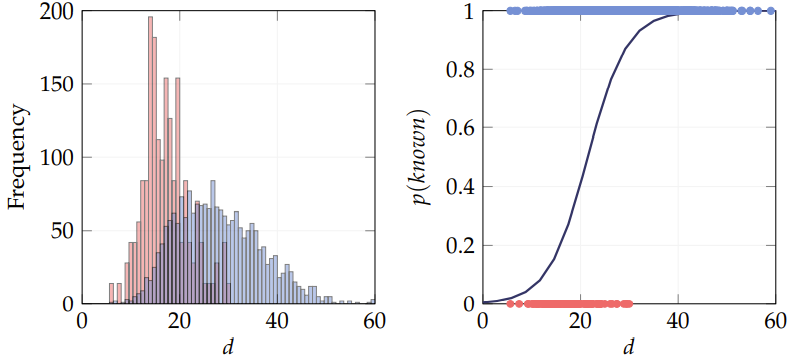
\includegraphics[width=0.9\textwidth]{setup12}
                \caption*{Setup 1}
            \end{subfigure}
            \begin{subfigure}{\textwidth}
                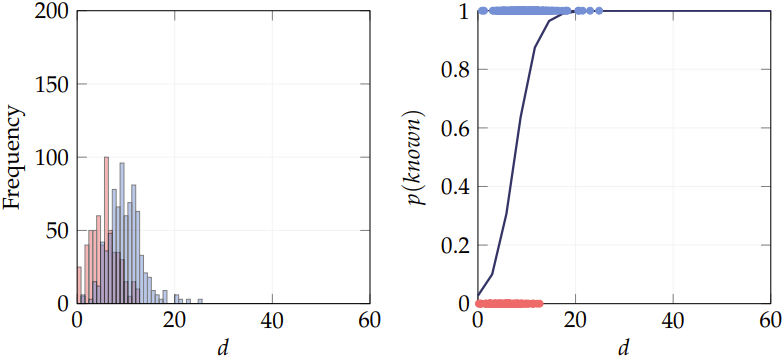
\includegraphics[width=0.9\textwidth]{setup22}
                \caption*{Setup 2}
            \end{subfigure} 
        \end{figure}
    \end{minipage}
    \hfill
    \begin{minipage}{0.45\textwidth}
        \begin{figure}
            \begin{subfigure}{\textwidth}
                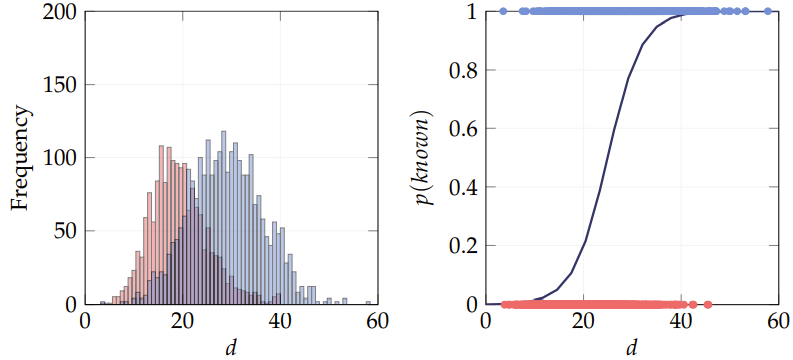
\includegraphics[width=0.9\textwidth]{setup3}
                \caption*{Setup 3}
            \end{subfigure}
            \begin{subfigure}{\textwidth}
                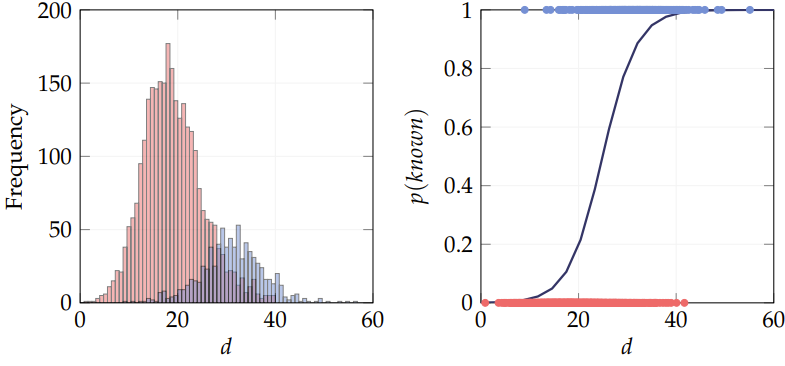
\includegraphics[width=0.9\textwidth]{setup4}
                \caption*{Setup 4}
            \end{subfigure}
        \end{figure}
    \end{minipage}
\end{frame}

\section{Conclusions}
%\begin{frame}{Conclusions}
    \begin{normalblock}{Conclusions and future outlook}
        \begin{itemize}
        \item <1-> The thesis explored OSR on a dataset composed of SEM images of wafer defects.
        \item <2-> A method based on Mahalanobis distance to detect novelties has been presented, which achieved modest results.
        \item <3-> The RPL framework, found in literature, has been tested and showed more promising results.
        \item <4-> Openness is not a good measure for the difficulty of the OSR task.
        \item <5-> Future directions include improving the organization of the dataset and exploring other possibilities, such as ARPL or Siamese Neural Networks.
        \end{itemize}
    \end{normalblock}
\end{frame}

\backmatter%

\appendix
\section{Additional Slides}
\begin{frame}{Activation Function}
    \begin{figure}[h]
        \begin{minipage}{0.28\textwidth}
        \centering
        \setlength\tabcolsep{0pt}
        \begin{tikzpicture}
            \pgfplotsset{%
                width=1.2\textwidth,
                height=1.2\textwidth
            }
            \begin{axis}[
                domain=-5:5,
                xlabel={$ReLU(x)$},
                samples=200,
                smooth,
            ]
            \addplot [
                domain=-5:0,
                red,
            ]
            {
                0
            };
            \addplot [
                domain=0:5,
                red,
            ]
            {
                x
            };
            \end{axis}
        \end{tikzpicture}
        \end{minipage}
        \begin{minipage}{0.28\textwidth}
        \centering
        \setlength\tabcolsep{0pt}
        \begin{tikzpicture}
            \pgfplotsset{%
                width=1.2\textwidth,
                height=1.2\textwidth
            }
            \begin{axis}[
                domain=-5:5,
                xlabel={$tanh(x)$},
                samples=200,
                smooth,
            ]
            \addplot [
                domain=-5:0,
                red,
            ]
            {
                tanh(x)
            };
            \addplot [
                domain=0:5,
                red,
            ]
            {
                tanh(x)
            };
            \end{axis}
        \end{tikzpicture}
        \end{minipage}
        \begin{minipage}{0.28\textwidth}
        \centering
        \setlength\tabcolsep{0pt}
        \begin{tikzpicture}
            \pgfplotsset{%
                width=1.2\textwidth,
                height=1.2\textwidth
            }
            \begin{axis}[
                domain=-5:5,
                xlabel={$\sigma(x)$},
                samples=200,
                smooth,
            ]
            \addplot [
                domain=-5:5,
                red,
            ]
            {
                1/(1+exp(-\x))
            };
            \end{axis}
        \end{tikzpicture}
        \end{minipage}
        \caption*{Activation Functions}
    \end{figure}
\end{frame}

\begin{frame}{ResNet50}
    \begin{table}[h]
        \scalebox{0.63}{
            \centering
            \setlength\extrarowheight{3pt}
            \begin{tabular}{|c|c|c|c|}
                \hline
                \textbf{Layer} & \textbf{Resolution} & \textbf{Channels} & \textbf{Layers} \\
                $\mathcal{F}_i$ & $H_i \times W_i$ & $C_i$ & $L_i$\\
                \hline
                Conv, $7\times7$, $s2$ & 112$\times$112 & 64 & 1 \\
                \hline
                Max Pool, $3 \times 3$, $s2$ & 56$\times$56 & 64 & 1 \\
                \hline
                $
                \begin{aligned}
                    & \text{Conv}, 1\times1 \\
                    & \text{Conv}, 3\times3 \\
                    & \text{Conv}, 1\times1 \\
                \end{aligned}
                $ & 56$\times$56 & $\begin{aligned} & 64 \\ & 64 \\ & 256 \\ \end{aligned}$ & 3 \\
                \hline
                $\begin{aligned}
                    & \text{Conv}, 1\times1 \\
                    & \text{Conv}, 3\times3 \\
                    & \text{Conv}, 1\times1 \\
                \end{aligned}
                $ & 28$\times$28 & $\begin{aligned} & 128 \\ & 128 \\ & 512 \\ \end{aligned}$ & 4 \\
                \hline
                $\begin{aligned}
                    & \text{Conv}, 1\times1 \\
                    & \text{Conv}, 3\times3 \\
                    & \text{Conv}, 1\times1 \\
                \end{aligned}
                $ & 14$\times$14 & $\begin{aligned} & 256 \\ & 256 \\ & 1024 \end{aligned} $ & 6 \\ \hline $\begin{aligned}
                    & \text{Conv}, 1\times1 \\
                    & \text{Conv}, 3\times3 \\
                    & \text{Conv}, 1\times1 \\
                \end{aligned}
                $ & 7$\times$7 & $\begin{aligned} & 512 \\ & 512 \\ & 2048 \\ \end{aligned}$ & 3 \\
                \hline 
                $\begin{aligned} & \text{Average Pool} \\ & \text{Fully-Connected} \end{aligned}$ & 1$\times$1 & 1000 & 1\\
                \hline 
            \end{tabular}
        }
            \caption*{ResNet50}
    \end{table}
\end{frame}

\begin{frame}{EfficientNet-B0}
    \begin{table}[h]
        \scalebox{0.7}{
            \centering
            \setlength\extrarowheight{3pt}
            \begin{tabular}{|c|c|c|c|}
                \hline
                \textbf{Layer} & \textbf{Resolution} & \textbf{Channels} & \textbf{Layers} \\
                $\mathcal{F}_i$ & $H_i \times W_i$ & $C_i$ & $L_i$\\
                \hline
                Conv, $3\times3$ & 224$\times$224 & 32 & 1 \\
                \hline
                MBConv, $3 \times 3$ & 112$\times$112 & 16 & 1 \\
                \hline
                MBConv, $3 \times 3$ & 112$\times$112 & 24 & 2 \\ 
                \hline 
                MBConv, $3 \times 3$ & 112$\times$112 & 24 & 2 \\
                \hline 
                MBConv, $5 \times 5$ & 56$\times$56 & 40 & 2 \\
                \hline 
                MBConv, $3 \times 3$ & 28$\times$28 & 80 & 3 \\
                \hline 
                MBConv, $5 \times 5$ & 14$\times$14 & 112 & 3 \\
                \hline 
                MBConv, $5 \times 5$ & 14$\times$14 & 192 & 4 \\
                \hline 
                MBConv, $3 \times 3$ & 7$\times$7 & 32 & 1 \\
                \hline 
                Conv, $1 \times 1$ & 7$\times$7 & 1280 & 1 \\
                \hline 
                $\begin{aligned} & \text{Average Pool} \\ & \text{Fully-Connected} \end{aligned}$ & 1$\times$1 & 1280 & 1\\
                \hline 
            \end{tabular}
            }
        \caption*{EfficientNet-B0}
    \end{table}
\end{frame}
\end{document}